\documentclass[twoside]{book}

% Packages required by doxygen
\usepackage{fixltx2e}
\usepackage{calc}
\usepackage{doxygen}
\usepackage[export]{adjustbox} % also loads graphicx
\usepackage{graphicx}
\usepackage[utf8]{inputenc}
\usepackage{makeidx}
\usepackage{multicol}
\usepackage{multirow}
\PassOptionsToPackage{warn}{textcomp}
\usepackage{textcomp}
\usepackage[nointegrals]{wasysym}
\usepackage[table]{xcolor}

% Font selection
\usepackage[T1]{fontenc}
\usepackage[scaled=.90]{helvet}
\usepackage{courier}
\usepackage{amssymb}
\usepackage{sectsty}
\renewcommand{\familydefault}{\sfdefault}
\allsectionsfont{%
  \fontseries{bc}\selectfont%
  \color{darkgray}%
}
\renewcommand{\DoxyLabelFont}{%
  \fontseries{bc}\selectfont%
  \color{darkgray}%
}
\newcommand{\+}{\discretionary{\mbox{\scriptsize$\hookleftarrow$}}{}{}}

% Page & text layout
\usepackage{geometry}
\geometry{%
  a4paper,%
  top=2.5cm,%
  bottom=2.5cm,%
  left=2.5cm,%
  right=2.5cm%
}
\tolerance=750
\hfuzz=15pt
\hbadness=750
\setlength{\emergencystretch}{15pt}
\setlength{\parindent}{0cm}
\setlength{\parskip}{3ex plus 2ex minus 2ex}
\makeatletter
\renewcommand{\paragraph}{%
  \@startsection{paragraph}{4}{0ex}{-1.0ex}{1.0ex}{%
    \normalfont\normalsize\bfseries\SS@parafont%
  }%
}
\renewcommand{\subparagraph}{%
  \@startsection{subparagraph}{5}{0ex}{-1.0ex}{1.0ex}{%
    \normalfont\normalsize\bfseries\SS@subparafont%
  }%
}
\makeatother

% Headers & footers
\usepackage{fancyhdr}
\pagestyle{fancyplain}
\fancyhead[LE]{\fancyplain{}{\bfseries\thepage}}
\fancyhead[CE]{\fancyplain{}{}}
\fancyhead[RE]{\fancyplain{}{\bfseries\leftmark}}
\fancyhead[LO]{\fancyplain{}{\bfseries\rightmark}}
\fancyhead[CO]{\fancyplain{}{}}
\fancyhead[RO]{\fancyplain{}{\bfseries\thepage}}
\fancyfoot[LE]{\fancyplain{}{}}
\fancyfoot[CE]{\fancyplain{}{}}
\fancyfoot[RE]{\fancyplain{}{\bfseries\scriptsize Generated by Doxygen }}
\fancyfoot[LO]{\fancyplain{}{\bfseries\scriptsize Generated by Doxygen }}
\fancyfoot[CO]{\fancyplain{}{}}
\fancyfoot[RO]{\fancyplain{}{}}
\renewcommand{\footrulewidth}{0.4pt}
\renewcommand{\chaptermark}[1]{%
  \markboth{#1}{}%
}
\renewcommand{\sectionmark}[1]{%
  \markright{\thesection\ #1}%
}

% Indices & bibliography
\usepackage{natbib}
\usepackage[titles]{tocloft}
\setcounter{tocdepth}{3}
\setcounter{secnumdepth}{5}
\makeindex

% Hyperlinks (required, but should be loaded last)
\usepackage{ifpdf}
\ifpdf
  \usepackage[pdftex,pagebackref=true]{hyperref}
\else
  \usepackage[ps2pdf,pagebackref=true]{hyperref}
\fi
\hypersetup{%
  colorlinks=true,%
  linkcolor=blue,%
  citecolor=blue,%
  unicode%
}

% Custom commands
\newcommand{\clearemptydoublepage}{%
  \newpage{\pagestyle{empty}\cleardoublepage}%
}

\usepackage{caption}
\captionsetup{labelsep=space,justification=centering,font={bf},singlelinecheck=off,skip=4pt,position=top}

%===== C O N T E N T S =====

\begin{document}

% Titlepage & ToC
\hypersetup{pageanchor=false,
             bookmarksnumbered=true,
             pdfencoding=unicode
            }
\pagenumbering{alph}
\begin{titlepage}
\vspace*{7cm}
\begin{center}%
{\Large Mouse-\/glove }\\
\vspace*{1cm}
{\large Generated by Doxygen 1.8.13}\\
\end{center}
\end{titlepage}
\clearemptydoublepage
\pagenumbering{roman}
\tableofcontents
\clearemptydoublepage
\pagenumbering{arabic}
\hypersetup{pageanchor=true}

%--- Begin generated contents ---
\chapter{Mouse-\/glove}
\label{index}\hypertarget{index}{}\subsection*{Project in Real Time Embedded Programming 5 (Team 15)}

\subsubsection*{Description}

In this project, the aim is to create a wireless glove that acts as a mouse. Users will be able to controll the pointer with the motion of their hand. Additional features of the Mouse-\/glove will enable users to make right and left clicks. Structural details of the system can be found below.



\subsubsection*{Members}


\begin{DoxyItemize}
\item Amina Gojak
\item Tong He
\item Yuzhen Liu
\end{DoxyItemize}

\subsubsection*{Packages/\+Libraries installation}


\begin{DoxyCode}
WiringPi: $sudo apt-get install wiringpi 
//For GPIO control and I2C  
\end{DoxyCode}
 
\begin{DoxyCode}
iir: https://github.com/berndporr/iir1 
//For iir filter 
\end{DoxyCode}
 
\begin{DoxyCode}
xdo: $sudo apt-get install -y libxdo-dev 
//For simulate mouse action
\end{DoxyCode}
 library for \hyperlink{classLSM9DS1}{L\+S\+M9\+D\+S1} has been integrated in the project.


\begin{DoxyCode}
boost test : sudo apt-get install libboost-all-dev 
//For unite testing
\end{DoxyCode}


\#\#\# Install 
\begin{DoxyCode}
mkdir build
cd build
cmake ..  
make
\end{DoxyCode}


\subsubsection*{Test}

After finish Install 
\begin{DoxyCode}
cd build  
make test
\end{DoxyCode}


\#\#\# Run 
\begin{DoxyCode}
cd bin  
./demo
\end{DoxyCode}


\href{https://gojakamina.github.io/Mouse-glove/}{\tt Documentation}

\href{https://twitter.com/glove_mouse}{\tt Follow us on twitter} 
\chapter{Hierarchical Index}
\section{Class Hierarchy}
This inheritance list is sorted roughly, but not completely, alphabetically\+:\begin{DoxyCompactList}
\item \contentsline{section}{accel\+Settings}{\pageref{structaccelSettings}}{}
\item \contentsline{section}{Cpp\+Timer}{\pageref{classCppTimer}}{}
\begin{DoxyCompactList}
\item \contentsline{section}{L\+S\+M9\+D\+S1}{\pageref{classLSM9DS1}}{}
\end{DoxyCompactList}
\item \contentsline{section}{device\+Settings}{\pageref{structdeviceSettings}}{}
\item \contentsline{section}{Filter}{\pageref{classFilter}}{}
\item \contentsline{section}{gyro\+Settings}{\pageref{structgyroSettings}}{}
\item \contentsline{section}{I\+M\+U\+Settings}{\pageref{structIMUSettings}}{}
\item \contentsline{section}{L\+S\+M9\+D\+S1callback}{\pageref{classLSM9DS1callback}}{}
\begin{DoxyCompactList}
\item \contentsline{section}{L\+S\+M9\+D\+S1\+Pos\+Data\+Callback}{\pageref{classLSM9DS1PosDataCallback}}{}
\end{DoxyCompactList}
\item \contentsline{section}{mag\+Settings}{\pageref{structmagSettings}}{}
\item \contentsline{section}{Mouse}{\pageref{classMouse}}{}
\item Q\+Widget\begin{DoxyCompactList}
\item \contentsline{section}{Instr\+Window}{\pageref{classInstrWindow}}{}
\item \contentsline{section}{Window}{\pageref{classWindow}}{}
\end{DoxyCompactList}
\item \contentsline{section}{temperature\+Settings}{\pageref{structtemperatureSettings}}{}
\end{DoxyCompactList}

\chapter{Class Index}
\section{Class List}
Here are the classes, structs, unions and interfaces with brief descriptions\+:\begin{DoxyCompactList}
\item\contentsline{section}{\hyperlink{structaccelSettings}{accel\+Settings} \\*Settings for accelerometer }{\pageref{structaccelSettings}}{}
\item\contentsline{section}{\hyperlink{classCppTimer}{Cpp\+Timer} \\*Software timer }{\pageref{classCppTimer}}{}
\item\contentsline{section}{\hyperlink{structdeviceSettings}{device\+Settings} \\*Device settings }{\pageref{structdeviceSettings}}{}
\item\contentsline{section}{\hyperlink{classFilter}{Filter} \\*Class that processes sensor data to position }{\pageref{classFilter}}{}
\item\contentsline{section}{\hyperlink{structgyroSettings}{gyro\+Settings} \\*Settings for gyroscope }{\pageref{structgyroSettings}}{}
\item\contentsline{section}{\hyperlink{structIMUSettings}{I\+M\+U\+Settings} \\*Settings for I\+MU }{\pageref{structIMUSettings}}{}
\item\contentsline{section}{\hyperlink{classInstrWindow}{Instr\+Window} \\*Instruction window class }{\pageref{classInstrWindow}}{}
\item\contentsline{section}{\hyperlink{classLSM9DS1}{L\+S\+M9\+D\+S1} \\*Class to enable sensor readings }{\pageref{classLSM9DS1}}{}
\item\contentsline{section}{\hyperlink{classLSM9DS1callback}{L\+S\+M9\+D\+S1callback} \\*Sensor data callback }{\pageref{classLSM9DS1callback}}{}
\item\contentsline{section}{\hyperlink{classLSM9DS1PosDataCallback}{L\+S\+M9\+D\+S1\+Pos\+Data\+Callback} \\*Position data callback }{\pageref{classLSM9DS1PosDataCallback}}{}
\item\contentsline{section}{\hyperlink{structmagSettings}{mag\+Settings} \\*Settings for magnetometer }{\pageref{structmagSettings}}{}
\item\contentsline{section}{\hyperlink{classMouse}{Mouse} \\*The class of mouse event including static functions called by interrupt }{\pageref{classMouse}}{}
\item\contentsline{section}{\hyperlink{structtemperatureSettings}{temperature\+Settings} \\*Settings for temperature }{\pageref{structtemperatureSettings}}{}
\item\contentsline{section}{\hyperlink{classWindow}{Window} \\*G\+UI window class }{\pageref{classWindow}}{}
\end{DoxyCompactList}

\chapter{Class Documentation}
\hypertarget{structaccelSettings}{}\section{accel\+Settings Struct Reference}
\label{structaccelSettings}\index{accel\+Settings@{accel\+Settings}}


Settings for accelerometer.  




{\ttfamily \#include $<$L\+S\+M9\+D\+S1\+\_\+\+Types.\+h$>$}



Collaboration diagram for accel\+Settings\+:\nopagebreak
\begin{figure}[H]
\begin{center}
\leavevmode
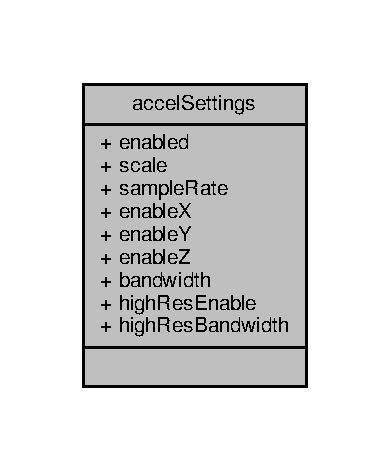
\includegraphics[width=187pt]{structaccelSettings__coll__graph}
\end{center}
\end{figure}
\subsection*{Public Attributes}
\begin{DoxyCompactItemize}
\item 
\mbox{\Hypertarget{structaccelSettings_a6ecaf7abfbaf7e74c6986fd93798ad4b}\label{structaccelSettings_a6ecaf7abfbaf7e74c6986fd93798ad4b}} 
uint8\+\_\+t \hyperlink{structaccelSettings_a6ecaf7abfbaf7e74c6986fd93798ad4b}{enabled}
\begin{DoxyCompactList}\small\item\em Enables readings. \end{DoxyCompactList}\item 
\mbox{\Hypertarget{structaccelSettings_a3a0a38e5e32ad21fcf8e880f37c0de1e}\label{structaccelSettings_a3a0a38e5e32ad21fcf8e880f37c0de1e}} 
uint8\+\_\+t \hyperlink{structaccelSettings_a3a0a38e5e32ad21fcf8e880f37c0de1e}{scale}
\begin{DoxyCompactList}\small\item\em Sets scale. \end{DoxyCompactList}\item 
\mbox{\Hypertarget{structaccelSettings_a51704cb40f1e72ec298f601fedcc6092}\label{structaccelSettings_a51704cb40f1e72ec298f601fedcc6092}} 
uint8\+\_\+t \hyperlink{structaccelSettings_a51704cb40f1e72ec298f601fedcc6092}{sample\+Rate}
\begin{DoxyCompactList}\small\item\em Sets sampling rate of readings. \end{DoxyCompactList}\item 
\mbox{\Hypertarget{structaccelSettings_a8cd5546cda8657ad2405d378fc815b9a}\label{structaccelSettings_a8cd5546cda8657ad2405d378fc815b9a}} 
uint8\+\_\+t \hyperlink{structaccelSettings_a8cd5546cda8657ad2405d378fc815b9a}{enableX}
\begin{DoxyCompactList}\small\item\em Enables x-\/readings. \end{DoxyCompactList}\item 
\mbox{\Hypertarget{structaccelSettings_a3f9ff5abfde83c5a59808faeb5ad4c6c}\label{structaccelSettings_a3f9ff5abfde83c5a59808faeb5ad4c6c}} 
uint8\+\_\+t \hyperlink{structaccelSettings_a3f9ff5abfde83c5a59808faeb5ad4c6c}{enableY}
\begin{DoxyCompactList}\small\item\em Enables y-\/readings. \end{DoxyCompactList}\item 
\mbox{\Hypertarget{structaccelSettings_abdb5ee5fb9a802315d8340ea5d83b587}\label{structaccelSettings_abdb5ee5fb9a802315d8340ea5d83b587}} 
uint8\+\_\+t \hyperlink{structaccelSettings_abdb5ee5fb9a802315d8340ea5d83b587}{enableZ}
\begin{DoxyCompactList}\small\item\em Enables z-\/readings. \end{DoxyCompactList}\item 
\mbox{\Hypertarget{structaccelSettings_ab64c80f62ecfeb3041744febaed9407b}\label{structaccelSettings_ab64c80f62ecfeb3041744febaed9407b}} 
int8\+\_\+t \hyperlink{structaccelSettings_ab64c80f62ecfeb3041744febaed9407b}{bandwidth}
\begin{DoxyCompactList}\small\item\em Sets bandwidth of readings. \end{DoxyCompactList}\item 
\mbox{\Hypertarget{structaccelSettings_ad165444ae7996ff6160be01d77d33b62}\label{structaccelSettings_ad165444ae7996ff6160be01d77d33b62}} 
uint8\+\_\+t \hyperlink{structaccelSettings_ad165444ae7996ff6160be01d77d33b62}{high\+Res\+Enable}
\begin{DoxyCompactList}\small\item\em Enables high resolution. \end{DoxyCompactList}\item 
\mbox{\Hypertarget{structaccelSettings_a3925a8342b5a4b3caecd187e729954f3}\label{structaccelSettings_a3925a8342b5a4b3caecd187e729954f3}} 
uint8\+\_\+t \hyperlink{structaccelSettings_a3925a8342b5a4b3caecd187e729954f3}{high\+Res\+Bandwidth}
\begin{DoxyCompactList}\small\item\em Enables high resolution in bandwidth. \end{DoxyCompactList}\end{DoxyCompactItemize}


\subsection{Detailed Description}
Settings for accelerometer. 

The documentation for this struct was generated from the following file\+:\begin{DoxyCompactItemize}
\item 
include/L\+S\+M9\+D\+S1\+\_\+\+Types.\+h\end{DoxyCompactItemize}

\hypertarget{classCppTimer}{}\section{Cpp\+Timer Class Reference}
\label{classCppTimer}\index{Cpp\+Timer@{Cpp\+Timer}}


Software timer.  




{\ttfamily \#include $<$Cpp\+Timer.\+h$>$}



Inheritance diagram for Cpp\+Timer\+:\nopagebreak
\begin{figure}[H]
\begin{center}
\leavevmode
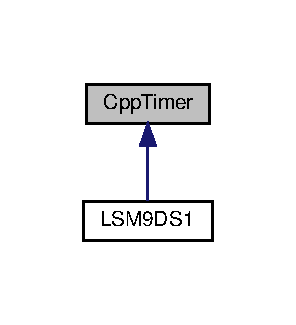
\includegraphics[height=550pt]{classCppTimer__inherit__graph}
\end{center}
\end{figure}


Collaboration diagram for Cpp\+Timer\+:\nopagebreak
\begin{figure}[H]
\begin{center}
\leavevmode
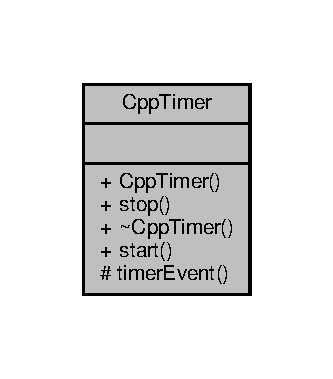
\includegraphics[width=160pt]{classCppTimer__coll__graph}
\end{center}
\end{figure}
\subsection*{Public Member Functions}
\begin{DoxyCompactItemize}
\item 
\mbox{\Hypertarget{classCppTimer_a327a07c051b9b60fcc61e6fd8f40f381}\label{classCppTimer_a327a07c051b9b60fcc61e6fd8f40f381}} 
\hyperlink{classCppTimer_a327a07c051b9b60fcc61e6fd8f40f381}{Cpp\+Timer} ()
\begin{DoxyCompactList}\small\item\em The constructor. \end{DoxyCompactList}\item 
\mbox{\Hypertarget{classCppTimer_a4bb95ddee98a536d0818b8f6096bf7e7}\label{classCppTimer_a4bb95ddee98a536d0818b8f6096bf7e7}} 
void \hyperlink{classCppTimer_a4bb95ddee98a536d0818b8f6096bf7e7}{stop} ()
\begin{DoxyCompactList}\small\item\em Stops and deletes the timer. \end{DoxyCompactList}\item 
\mbox{\Hypertarget{classCppTimer_a2942aab831713273a76218048fe61b16}\label{classCppTimer_a2942aab831713273a76218048fe61b16}} 
virtual \hyperlink{classCppTimer_a2942aab831713273a76218048fe61b16}{$\sim$\+Cpp\+Timer} ()
\begin{DoxyCompactList}\small\item\em The destructor. \end{DoxyCompactList}\item 
\mbox{\Hypertarget{classCppTimer_a8d284721892e8e2665433f17045143e8}\label{classCppTimer_a8d284721892e8e2665433f17045143e8}} 
void \hyperlink{classCppTimer_a8d284721892e8e2665433f17045143e8}{start} (long nanosecs)
\begin{DoxyCompactList}\small\item\em Starts the timer. \end{DoxyCompactList}\end{DoxyCompactItemize}
\subsection*{Protected Member Functions}
\begin{DoxyCompactItemize}
\item 
virtual void \hyperlink{classCppTimer_ac2665403595b6aee5f581d0ebfeb886c}{timer\+Event} ()=0
\begin{DoxyCompactList}\small\item\em The timerevent. \end{DoxyCompactList}\end{DoxyCompactItemize}


\subsection{Detailed Description}
Software timer. 

\subsection{Member Function Documentation}
\mbox{\Hypertarget{classCppTimer_ac2665403595b6aee5f581d0ebfeb886c}\label{classCppTimer_ac2665403595b6aee5f581d0ebfeb886c}} 
\index{Cpp\+Timer@{Cpp\+Timer}!timer\+Event@{timer\+Event}}
\index{timer\+Event@{timer\+Event}!Cpp\+Timer@{Cpp\+Timer}}
\subsubsection{\texorpdfstring{timer\+Event()}{timerEvent()}}
{\footnotesize\ttfamily virtual void Cpp\+Timer\+::timer\+Event (\begin{DoxyParamCaption}{ }\end{DoxyParamCaption})\hspace{0.3cm}{\ttfamily [protected]}, {\ttfamily [pure virtual]}}



The timerevent. 

It is implemented by its children and executes once start method has been called. 

Implemented in \hyperlink{classLSM9DS1_ad1fffc2bc5987339430d3b293da0bdd1}{L\+S\+M9\+D\+S1}.

Here is the caller graph for this function\+:\nopagebreak
\begin{figure}[H]
\begin{center}
\leavevmode
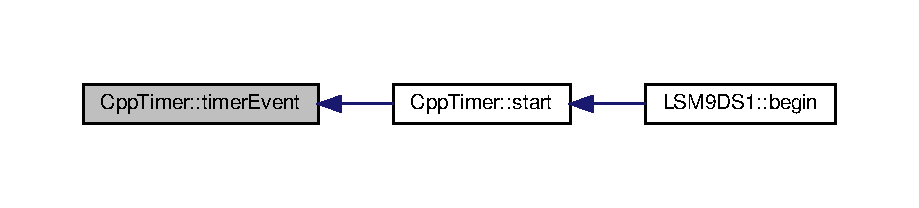
\includegraphics[width=350pt]{classCppTimer_ac2665403595b6aee5f581d0ebfeb886c_icgraph}
\end{center}
\end{figure}


The documentation for this class was generated from the following file\+:\begin{DoxyCompactItemize}
\item 
include/Cpp\+Timer.\+h\end{DoxyCompactItemize}

\hypertarget{structdeviceSettings}{}\section{device\+Settings Struct Reference}
\label{structdeviceSettings}\index{device\+Settings@{device\+Settings}}


Device settings.  




{\ttfamily \#include $<$L\+S\+M9\+D\+S1\+\_\+\+Types.\+h$>$}

\subsection*{Public Attributes}
\begin{DoxyCompactItemize}
\item 
\mbox{\Hypertarget{structdeviceSettings_a6512c63d06cce5f99760b1b3a6a4dfe9}\label{structdeviceSettings_a6512c63d06cce5f99760b1b3a6a4dfe9}} 
uint8\+\_\+t \hyperlink{structdeviceSettings_a6512c63d06cce5f99760b1b3a6a4dfe9}{comm\+Interface}
\begin{DoxyCompactList}\small\item\em Sets common interface. \end{DoxyCompactList}\item 
\mbox{\Hypertarget{structdeviceSettings_a2f43ac785e01fcbcfaf8436885f638ab}\label{structdeviceSettings_a2f43ac785e01fcbcfaf8436885f638ab}} 
uint8\+\_\+t \hyperlink{structdeviceSettings_a2f43ac785e01fcbcfaf8436885f638ab}{ag\+Address}
\begin{DoxyCompactList}\small\item\em Sets address of I2C or S\+PI CS pin. \end{DoxyCompactList}\item 
\mbox{\Hypertarget{structdeviceSettings_aec4e1d3e3f38b4e3e0f74f1640e16faa}\label{structdeviceSettings_aec4e1d3e3f38b4e3e0f74f1640e16faa}} 
uint8\+\_\+t \hyperlink{structdeviceSettings_aec4e1d3e3f38b4e3e0f74f1640e16faa}{m\+Address}
\begin{DoxyCompactList}\small\item\em Sets address of I2C or S\+PI CS pin. \end{DoxyCompactList}\end{DoxyCompactItemize}


\subsection{Detailed Description}
Device settings. 

The documentation for this struct was generated from the following file\+:\begin{DoxyCompactItemize}
\item 
include/L\+S\+M9\+D\+S1\+\_\+\+Types.\+h\end{DoxyCompactItemize}

\hypertarget{classFilter}{}\section{Filter Class Reference}
\label{classFilter}\index{Filter@{Filter}}


Class that processes sensor data to position.  




{\ttfamily \#include $<$Filter.\+h$>$}



Collaboration diagram for Filter\+:\nopagebreak
\begin{figure}[H]
\begin{center}
\leavevmode
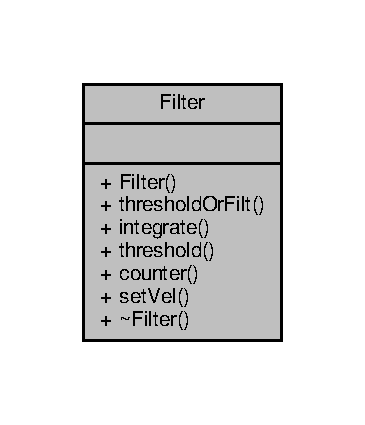
\includegraphics[width=175pt]{classFilter__coll__graph}
\end{center}
\end{figure}
\subsection*{Public Member Functions}
\begin{DoxyCompactItemize}
\item 
\hyperlink{classFilter_ad15994c30d497afd567a6445446a249e}{Filter} ()
\item 
float \hyperlink{classFilter_a4cf317f524d27d1257dcd1defc55b60d}{threshold\+Or\+Filt} (float value)
\begin{DoxyCompactList}\small\item\em Threshold and filter used for accelerometer data. \end{DoxyCompactList}\item 
float \hyperlink{classFilter_a7cf738197eb1c4db4da770bb3caba0cc}{integrate} (float val0, float curr, float prev)
\begin{DoxyCompactList}\small\item\em Integrates the input value with the trapezoidal method. \end{DoxyCompactList}\item 
void \hyperlink{classFilter_a6a1278398f661776ec6e2d11c527efbd}{threshold} (float \&value, float \&prev)
\begin{DoxyCompactList}\small\item\em Threshold used for velocity data that prevents drift and acts as a hp filter. \end{DoxyCompactList}\item 
void \hyperlink{classFilter_af82d470c92431795b69c0bda29ceb534}{counter} (int \&count, float accel)
\begin{DoxyCompactList}\small\item\em Counts number of times that acceleration has been zero. \end{DoxyCompactList}\item 
void \hyperlink{classFilter_a37eff97b71271134bb8dce35947893d2}{set\+Vel} (int \&\hyperlink{classFilter_af82d470c92431795b69c0bda29ceb534}{counter}, float \&vel, float \&prev\+Vel)
\begin{DoxyCompactList}\small\item\em Sets current and previous velocity value to zero if the counter has exceeded 5. \end{DoxyCompactList}\item 
\hyperlink{classFilter_a502ee334d42eac3edbaf32b599f9c35e}{$\sim$\+Filter} ()
\end{DoxyCompactItemize}


\subsection{Detailed Description}
Class that processes sensor data to position. 

\subsection{Constructor \& Destructor Documentation}
\mbox{\Hypertarget{classFilter_ad15994c30d497afd567a6445446a249e}\label{classFilter_ad15994c30d497afd567a6445446a249e}} 
\index{Filter@{Filter}!Filter@{Filter}}
\index{Filter@{Filter}!Filter@{Filter}}
\subsubsection{\texorpdfstring{Filter()}{Filter()}}
{\footnotesize\ttfamily Filter\+::\+Filter (\begin{DoxyParamCaption}{ }\end{DoxyParamCaption})}

The constructor. \mbox{\Hypertarget{classFilter_a502ee334d42eac3edbaf32b599f9c35e}\label{classFilter_a502ee334d42eac3edbaf32b599f9c35e}} 
\index{Filter@{Filter}!````~Filter@{$\sim$\+Filter}}
\index{````~Filter@{$\sim$\+Filter}!Filter@{Filter}}
\subsubsection{\texorpdfstring{$\sim$\+Filter()}{~Filter()}}
{\footnotesize\ttfamily Filter\+::$\sim$\+Filter (\begin{DoxyParamCaption}{ }\end{DoxyParamCaption})}

The destructor. 

\subsection{Member Function Documentation}
\mbox{\Hypertarget{classFilter_af82d470c92431795b69c0bda29ceb534}\label{classFilter_af82d470c92431795b69c0bda29ceb534}} 
\index{Filter@{Filter}!counter@{counter}}
\index{counter@{counter}!Filter@{Filter}}
\subsubsection{\texorpdfstring{counter()}{counter()}}
{\footnotesize\ttfamily void Filter\+::counter (\begin{DoxyParamCaption}\item[{int \&}]{count,  }\item[{float}]{accel }\end{DoxyParamCaption})}



Counts number of times that acceleration has been zero. 


\begin{DoxyParams}{Parameters}
{\em count} & the counter that is checked. \\
\hline
{\em accel} & the value of the current acceleration. \\
\hline
\end{DoxyParams}
\mbox{\Hypertarget{classFilter_a7cf738197eb1c4db4da770bb3caba0cc}\label{classFilter_a7cf738197eb1c4db4da770bb3caba0cc}} 
\index{Filter@{Filter}!integrate@{integrate}}
\index{integrate@{integrate}!Filter@{Filter}}
\subsubsection{\texorpdfstring{integrate()}{integrate()}}
{\footnotesize\ttfamily float Filter\+::integrate (\begin{DoxyParamCaption}\item[{float}]{val0,  }\item[{float}]{curr,  }\item[{float}]{prev }\end{DoxyParamCaption})}



Integrates the input value with the trapezoidal method. 


\begin{DoxyParams}{Parameters}
{\em val0} & the initial value. \\
\hline
{\em curr} & the current value with unit that needs to be integrated. \\
\hline
{\em prev} & the previous value with unit that needs to be integrated. \\
\hline
\end{DoxyParams}
\begin{DoxyReturn}{Returns}
the calculated integral. 
\end{DoxyReturn}
\mbox{\Hypertarget{classFilter_a37eff97b71271134bb8dce35947893d2}\label{classFilter_a37eff97b71271134bb8dce35947893d2}} 
\index{Filter@{Filter}!set\+Vel@{set\+Vel}}
\index{set\+Vel@{set\+Vel}!Filter@{Filter}}
\subsubsection{\texorpdfstring{set\+Vel()}{setVel()}}
{\footnotesize\ttfamily void Filter\+::set\+Vel (\begin{DoxyParamCaption}\item[{int \&}]{counter,  }\item[{float \&}]{vel,  }\item[{float \&}]{prev\+Vel }\end{DoxyParamCaption})}



Sets current and previous velocity value to zero if the counter has exceeded 5. 


\begin{DoxyParams}{Parameters}
{\em counter} & the counter that is checked. \\
\hline
{\em vel} & the current velocity. \\
\hline
{\em prev\+Vel} & the previous velocity. \\
\hline
\end{DoxyParams}
\mbox{\Hypertarget{classFilter_a6a1278398f661776ec6e2d11c527efbd}\label{classFilter_a6a1278398f661776ec6e2d11c527efbd}} 
\index{Filter@{Filter}!threshold@{threshold}}
\index{threshold@{threshold}!Filter@{Filter}}
\subsubsection{\texorpdfstring{threshold()}{threshold()}}
{\footnotesize\ttfamily void Filter\+::threshold (\begin{DoxyParamCaption}\item[{float \&}]{value,  }\item[{float \&}]{prev }\end{DoxyParamCaption})}



Threshold used for velocity data that prevents drift and acts as a hp filter. 

If the value doesn\textquotesingle{}t reach threshold, both the current value and previous will be set to 0.


\begin{DoxyParams}{Parameters}
{\em value} & the input value that should be checked. \\
\hline
{\em prev} & the previous value corresponding to the input value. \\
\hline
\end{DoxyParams}
\mbox{\Hypertarget{classFilter_a4cf317f524d27d1257dcd1defc55b60d}\label{classFilter_a4cf317f524d27d1257dcd1defc55b60d}} 
\index{Filter@{Filter}!threshold\+Or\+Filt@{threshold\+Or\+Filt}}
\index{threshold\+Or\+Filt@{threshold\+Or\+Filt}!Filter@{Filter}}
\subsubsection{\texorpdfstring{threshold\+Or\+Filt()}{thresholdOrFilt()}}
{\footnotesize\ttfamily float Filter\+::threshold\+Or\+Filt (\begin{DoxyParamCaption}\item[{float}]{value }\end{DoxyParamCaption})}



Threshold and filter used for accelerometer data. 

If the threshold is reached the data will be lowpass filtered.


\begin{DoxyParams}{Parameters}
{\em value} & the input value that should be processed. \\
\hline
\end{DoxyParams}
\begin{DoxyReturn}{Returns}
0 if the value doesn\textquotesingle{}t reach threshold, otherwise return lowpass filtered value. 
\end{DoxyReturn}


The documentation for this class was generated from the following files\+:\begin{DoxyCompactItemize}
\item 
include/Filter.\+h\item 
src/Filter.\+cpp\end{DoxyCompactItemize}

\hypertarget{structgyroSettings}{}\section{gyro\+Settings Struct Reference}
\label{structgyroSettings}\index{gyro\+Settings@{gyro\+Settings}}


Settings for gyroscope.  




{\ttfamily \#include $<$L\+S\+M9\+D\+S1\+\_\+\+Types.\+h$>$}



Collaboration diagram for gyro\+Settings\+:\nopagebreak
\begin{figure}[H]
\begin{center}
\leavevmode
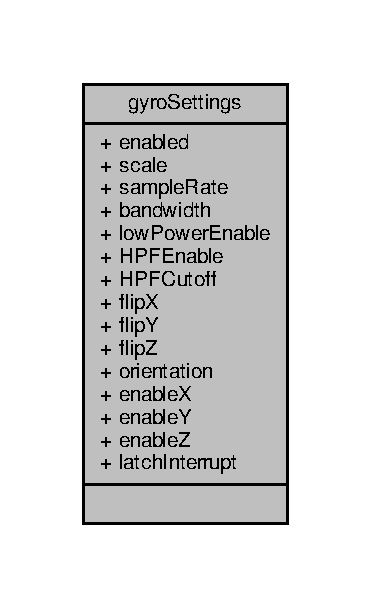
\includegraphics[width=178pt]{structgyroSettings__coll__graph}
\end{center}
\end{figure}
\subsection*{Public Attributes}
\begin{DoxyCompactItemize}
\item 
\mbox{\Hypertarget{structgyroSettings_ac9c769eeefed971baac74a7b81b25e7b}\label{structgyroSettings_ac9c769eeefed971baac74a7b81b25e7b}} 
uint8\+\_\+t \hyperlink{structgyroSettings_ac9c769eeefed971baac74a7b81b25e7b}{enabled}
\begin{DoxyCompactList}\small\item\em Enables readings. \end{DoxyCompactList}\item 
\mbox{\Hypertarget{structgyroSettings_a70ced5c47e97d4dd6770954117ad3a9f}\label{structgyroSettings_a70ced5c47e97d4dd6770954117ad3a9f}} 
uint16\+\_\+t \hyperlink{structgyroSettings_a70ced5c47e97d4dd6770954117ad3a9f}{scale}
\begin{DoxyCompactList}\small\item\em Sets scale. \end{DoxyCompactList}\item 
\mbox{\Hypertarget{structgyroSettings_a58ebac4d1f242d6b129570396a7355b0}\label{structgyroSettings_a58ebac4d1f242d6b129570396a7355b0}} 
uint8\+\_\+t \hyperlink{structgyroSettings_a58ebac4d1f242d6b129570396a7355b0}{sample\+Rate}
\begin{DoxyCompactList}\small\item\em Sets sampling rate of readings. \end{DoxyCompactList}\item 
\mbox{\Hypertarget{structgyroSettings_ac3f0782333ec55165c1f589d445ba374}\label{structgyroSettings_ac3f0782333ec55165c1f589d445ba374}} 
uint8\+\_\+t \hyperlink{structgyroSettings_ac3f0782333ec55165c1f589d445ba374}{bandwidth}
\begin{DoxyCompactList}\small\item\em Sets bandwidth of readings. \end{DoxyCompactList}\item 
\mbox{\Hypertarget{structgyroSettings_a296a167235d876fa79afc471399e763b}\label{structgyroSettings_a296a167235d876fa79afc471399e763b}} 
uint8\+\_\+t \hyperlink{structgyroSettings_a296a167235d876fa79afc471399e763b}{low\+Power\+Enable}
\begin{DoxyCompactList}\small\item\em Enables low power. \end{DoxyCompactList}\item 
\mbox{\Hypertarget{structgyroSettings_aa7aa5eba55588e4bcfc0be9ea9b6ed8d}\label{structgyroSettings_aa7aa5eba55588e4bcfc0be9ea9b6ed8d}} 
uint8\+\_\+t \hyperlink{structgyroSettings_aa7aa5eba55588e4bcfc0be9ea9b6ed8d}{H\+P\+F\+Enable}
\begin{DoxyCompactList}\small\item\em Enables high pass filter. \end{DoxyCompactList}\item 
\mbox{\Hypertarget{structgyroSettings_a7357a9b858fdf515e969ae4e06459f37}\label{structgyroSettings_a7357a9b858fdf515e969ae4e06459f37}} 
uint8\+\_\+t \hyperlink{structgyroSettings_a7357a9b858fdf515e969ae4e06459f37}{H\+P\+F\+Cutoff}
\begin{DoxyCompactList}\small\item\em Sets high pass filter cutoff frequency. \end{DoxyCompactList}\item 
\mbox{\Hypertarget{structgyroSettings_a877b529e39287bed155acbca97a75540}\label{structgyroSettings_a877b529e39287bed155acbca97a75540}} 
uint8\+\_\+t \hyperlink{structgyroSettings_a877b529e39287bed155acbca97a75540}{flipX}
\begin{DoxyCompactList}\small\item\em Flips x readings. \end{DoxyCompactList}\item 
\mbox{\Hypertarget{structgyroSettings_a2137659e07899a0efccc941e003c07e0}\label{structgyroSettings_a2137659e07899a0efccc941e003c07e0}} 
uint8\+\_\+t \hyperlink{structgyroSettings_a2137659e07899a0efccc941e003c07e0}{flipY}
\begin{DoxyCompactList}\small\item\em Flips y readings. \end{DoxyCompactList}\item 
\mbox{\Hypertarget{structgyroSettings_a94c92be9f7c56dd9cd21120307d7373f}\label{structgyroSettings_a94c92be9f7c56dd9cd21120307d7373f}} 
uint8\+\_\+t \hyperlink{structgyroSettings_a94c92be9f7c56dd9cd21120307d7373f}{flipZ}
\begin{DoxyCompactList}\small\item\em Flips z readings. \end{DoxyCompactList}\item 
\mbox{\Hypertarget{structgyroSettings_a33239fd5c4a0fd74670455008c2701ee}\label{structgyroSettings_a33239fd5c4a0fd74670455008c2701ee}} 
uint8\+\_\+t \hyperlink{structgyroSettings_a33239fd5c4a0fd74670455008c2701ee}{orientation}
\begin{DoxyCompactList}\small\item\em Sets the gyro orientation. \end{DoxyCompactList}\item 
\mbox{\Hypertarget{structgyroSettings_a7c1000d1151579743faa376d49751f1d}\label{structgyroSettings_a7c1000d1151579743faa376d49751f1d}} 
uint8\+\_\+t \hyperlink{structgyroSettings_a7c1000d1151579743faa376d49751f1d}{enableX}
\begin{DoxyCompactList}\small\item\em Enables x-\/readings. \end{DoxyCompactList}\item 
\mbox{\Hypertarget{structgyroSettings_a4d6ea95b7a52daab6d48dc128c83f3d8}\label{structgyroSettings_a4d6ea95b7a52daab6d48dc128c83f3d8}} 
uint8\+\_\+t \hyperlink{structgyroSettings_a4d6ea95b7a52daab6d48dc128c83f3d8}{enableY}
\begin{DoxyCompactList}\small\item\em Enables y-\/readings. \end{DoxyCompactList}\item 
\mbox{\Hypertarget{structgyroSettings_a86a86182fd841bd651672d43803b5c63}\label{structgyroSettings_a86a86182fd841bd651672d43803b5c63}} 
uint8\+\_\+t \hyperlink{structgyroSettings_a86a86182fd841bd651672d43803b5c63}{enableZ}
\begin{DoxyCompactList}\small\item\em Enables z-\/readings. \end{DoxyCompactList}\item 
\mbox{\Hypertarget{structgyroSettings_a3eb9f52cae013b107fbc5059220f9333}\label{structgyroSettings_a3eb9f52cae013b107fbc5059220f9333}} 
uint8\+\_\+t \hyperlink{structgyroSettings_a3eb9f52cae013b107fbc5059220f9333}{latch\+Interrupt}
\begin{DoxyCompactList}\small\item\em Enables latch interrupt. \end{DoxyCompactList}\end{DoxyCompactItemize}


\subsection{Detailed Description}
Settings for gyroscope. 

The documentation for this struct was generated from the following file\+:\begin{DoxyCompactItemize}
\item 
include/L\+S\+M9\+D\+S1\+\_\+\+Types.\+h\end{DoxyCompactItemize}

\hypertarget{structIMUSettings}{}\section{I\+M\+U\+Settings Struct Reference}
\label{structIMUSettings}\index{I\+M\+U\+Settings@{I\+M\+U\+Settings}}


Settings for I\+MU.  




{\ttfamily \#include $<$L\+S\+M9\+D\+S1\+\_\+\+Types.\+h$>$}



Collaboration diagram for I\+M\+U\+Settings\+:\nopagebreak
\begin{figure}[H]
\begin{center}
\leavevmode
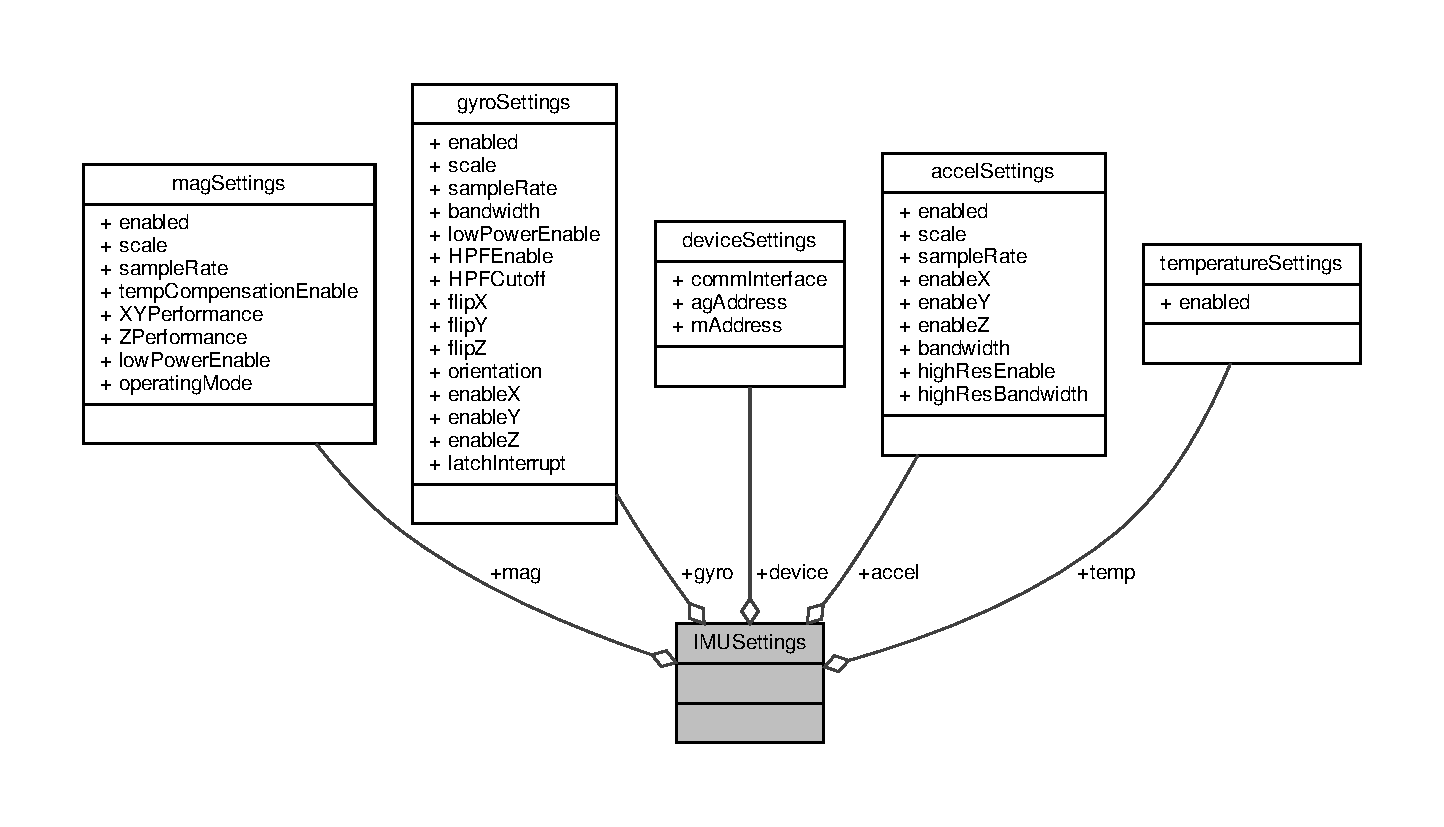
\includegraphics[width=350pt]{structIMUSettings__coll__graph}
\end{center}
\end{figure}
\subsection*{Public Attributes}
\begin{DoxyCompactItemize}
\item 
\mbox{\Hypertarget{structIMUSettings_a22b2648befc58307b43edc9e74acd583}\label{structIMUSettings_a22b2648befc58307b43edc9e74acd583}} 
\hyperlink{structdeviceSettings}{device\+Settings} \hyperlink{structIMUSettings_a22b2648befc58307b43edc9e74acd583}{device}
\begin{DoxyCompactList}\small\item\em Sets device. \end{DoxyCompactList}\item 
\mbox{\Hypertarget{structIMUSettings_afab65feef7d0ca778b035a8805b1e4bf}\label{structIMUSettings_afab65feef7d0ca778b035a8805b1e4bf}} 
\hyperlink{structgyroSettings}{gyro\+Settings} \hyperlink{structIMUSettings_afab65feef7d0ca778b035a8805b1e4bf}{gyro}
\begin{DoxyCompactList}\small\item\em Sets gyroscope settings. \end{DoxyCompactList}\item 
\mbox{\Hypertarget{structIMUSettings_aa8c7bf392c70397ae02ee1f5ad0ea474}\label{structIMUSettings_aa8c7bf392c70397ae02ee1f5ad0ea474}} 
\hyperlink{structaccelSettings}{accel\+Settings} \hyperlink{structIMUSettings_aa8c7bf392c70397ae02ee1f5ad0ea474}{accel}
\begin{DoxyCompactList}\small\item\em Sets accelerometer settings. \end{DoxyCompactList}\item 
\mbox{\Hypertarget{structIMUSettings_aca08359dfa3b8120aa687680d6c06ba7}\label{structIMUSettings_aca08359dfa3b8120aa687680d6c06ba7}} 
\hyperlink{structmagSettings}{mag\+Settings} \hyperlink{structIMUSettings_aca08359dfa3b8120aa687680d6c06ba7}{mag}
\begin{DoxyCompactList}\small\item\em Sets magnetometer settings. \end{DoxyCompactList}\item 
\mbox{\Hypertarget{structIMUSettings_a55a77555f1843c186db02080078632f2}\label{structIMUSettings_a55a77555f1843c186db02080078632f2}} 
\hyperlink{structtemperatureSettings}{temperature\+Settings} \hyperlink{structIMUSettings_a55a77555f1843c186db02080078632f2}{temp}
\begin{DoxyCompactList}\small\item\em Sets temperature settings. \end{DoxyCompactList}\end{DoxyCompactItemize}


\subsection{Detailed Description}
Settings for I\+MU. 

The documentation for this struct was generated from the following file\+:\begin{DoxyCompactItemize}
\item 
include/L\+S\+M9\+D\+S1\+\_\+\+Types.\+h\end{DoxyCompactItemize}

\hypertarget{classInstrWindow}{}\section{Instr\+Window Class Reference}
\label{classInstrWindow}\index{Instr\+Window@{Instr\+Window}}


Instruction window class.  




{\ttfamily \#include $<$instrwindow.\+h$>$}



Inheritance diagram for Instr\+Window\+:\nopagebreak
\begin{figure}[H]
\begin{center}
\leavevmode
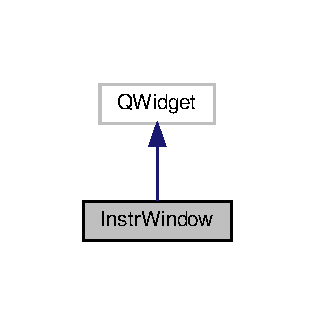
\includegraphics[width=172pt]{classInstrWindow__inherit__graph}
\end{center}
\end{figure}


Collaboration diagram for Instr\+Window\+:\nopagebreak
\begin{figure}[H]
\begin{center}
\leavevmode
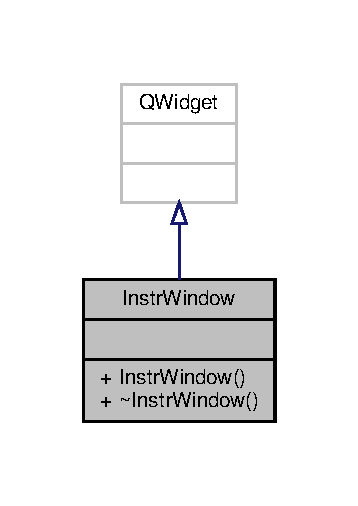
\includegraphics[width=172pt]{classInstrWindow__coll__graph}
\end{center}
\end{figure}
\subsection*{Public Member Functions}
\begin{DoxyCompactItemize}
\item 
\hyperlink{classInstrWindow_a4d425c2334a77bdc9e3f0aa91e691909}{Instr\+Window} ()
\item 
\hyperlink{classInstrWindow_a192ae02056142b9567d9c87c0708f7a5}{$\sim$\+Instr\+Window} ()
\end{DoxyCompactItemize}


\subsection{Detailed Description}
Instruction window class. 

\subsection{Constructor \& Destructor Documentation}
\mbox{\Hypertarget{classInstrWindow_a4d425c2334a77bdc9e3f0aa91e691909}\label{classInstrWindow_a4d425c2334a77bdc9e3f0aa91e691909}} 
\index{Instr\+Window@{Instr\+Window}!Instr\+Window@{Instr\+Window}}
\index{Instr\+Window@{Instr\+Window}!Instr\+Window@{Instr\+Window}}
\subsubsection{\texorpdfstring{Instr\+Window()}{InstrWindow()}}
{\footnotesize\ttfamily Instr\+Window\+::\+Instr\+Window (\begin{DoxyParamCaption}{ }\end{DoxyParamCaption})}

The constructor. \mbox{\Hypertarget{classInstrWindow_a192ae02056142b9567d9c87c0708f7a5}\label{classInstrWindow_a192ae02056142b9567d9c87c0708f7a5}} 
\index{Instr\+Window@{Instr\+Window}!````~Instr\+Window@{$\sim$\+Instr\+Window}}
\index{````~Instr\+Window@{$\sim$\+Instr\+Window}!Instr\+Window@{Instr\+Window}}
\subsubsection{\texorpdfstring{$\sim$\+Instr\+Window()}{~InstrWindow()}}
{\footnotesize\ttfamily Instr\+Window\+::$\sim$\+Instr\+Window (\begin{DoxyParamCaption}{ }\end{DoxyParamCaption})}

The destructor. 

The documentation for this class was generated from the following files\+:\begin{DoxyCompactItemize}
\item 
G\+U\+I/instrwindow.\+h\item 
G\+U\+I/instrwindow.\+cpp\end{DoxyCompactItemize}

\hypertarget{classLSM9DS1}{}\section{L\+S\+M9\+D\+S1 Class Reference}
\label{classLSM9DS1}\index{L\+S\+M9\+D\+S1@{L\+S\+M9\+D\+S1}}


Class to enable sensor readings.  




{\ttfamily \#include $<$L\+S\+M9\+D\+S1.\+h$>$}



Inheritance diagram for L\+S\+M9\+D\+S1\+:\nopagebreak
\begin{figure}[H]
\begin{center}
\leavevmode
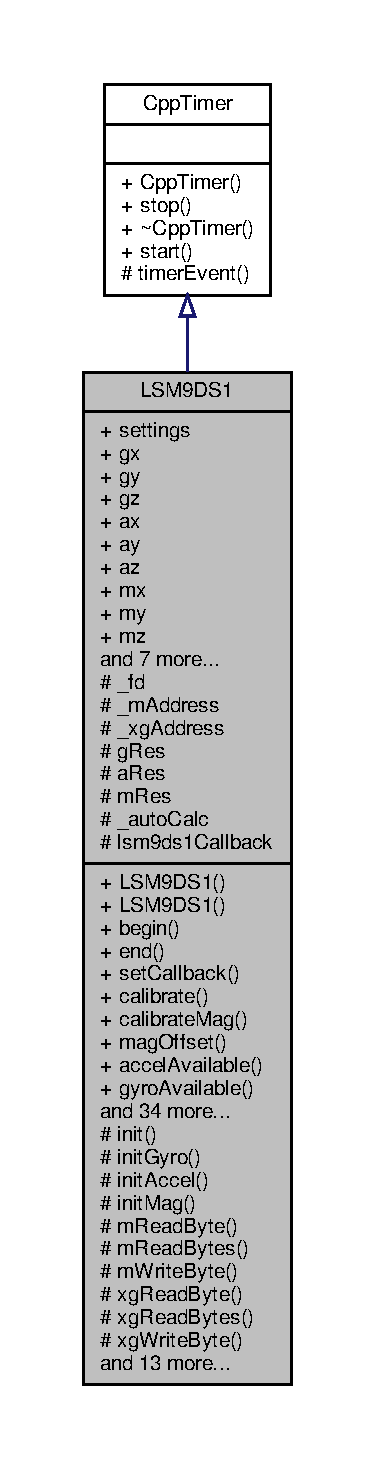
\includegraphics[height=550pt]{classLSM9DS1__inherit__graph}
\end{center}
\end{figure}


Collaboration diagram for L\+S\+M9\+D\+S1\+:\nopagebreak
\begin{figure}[H]
\begin{center}
\leavevmode
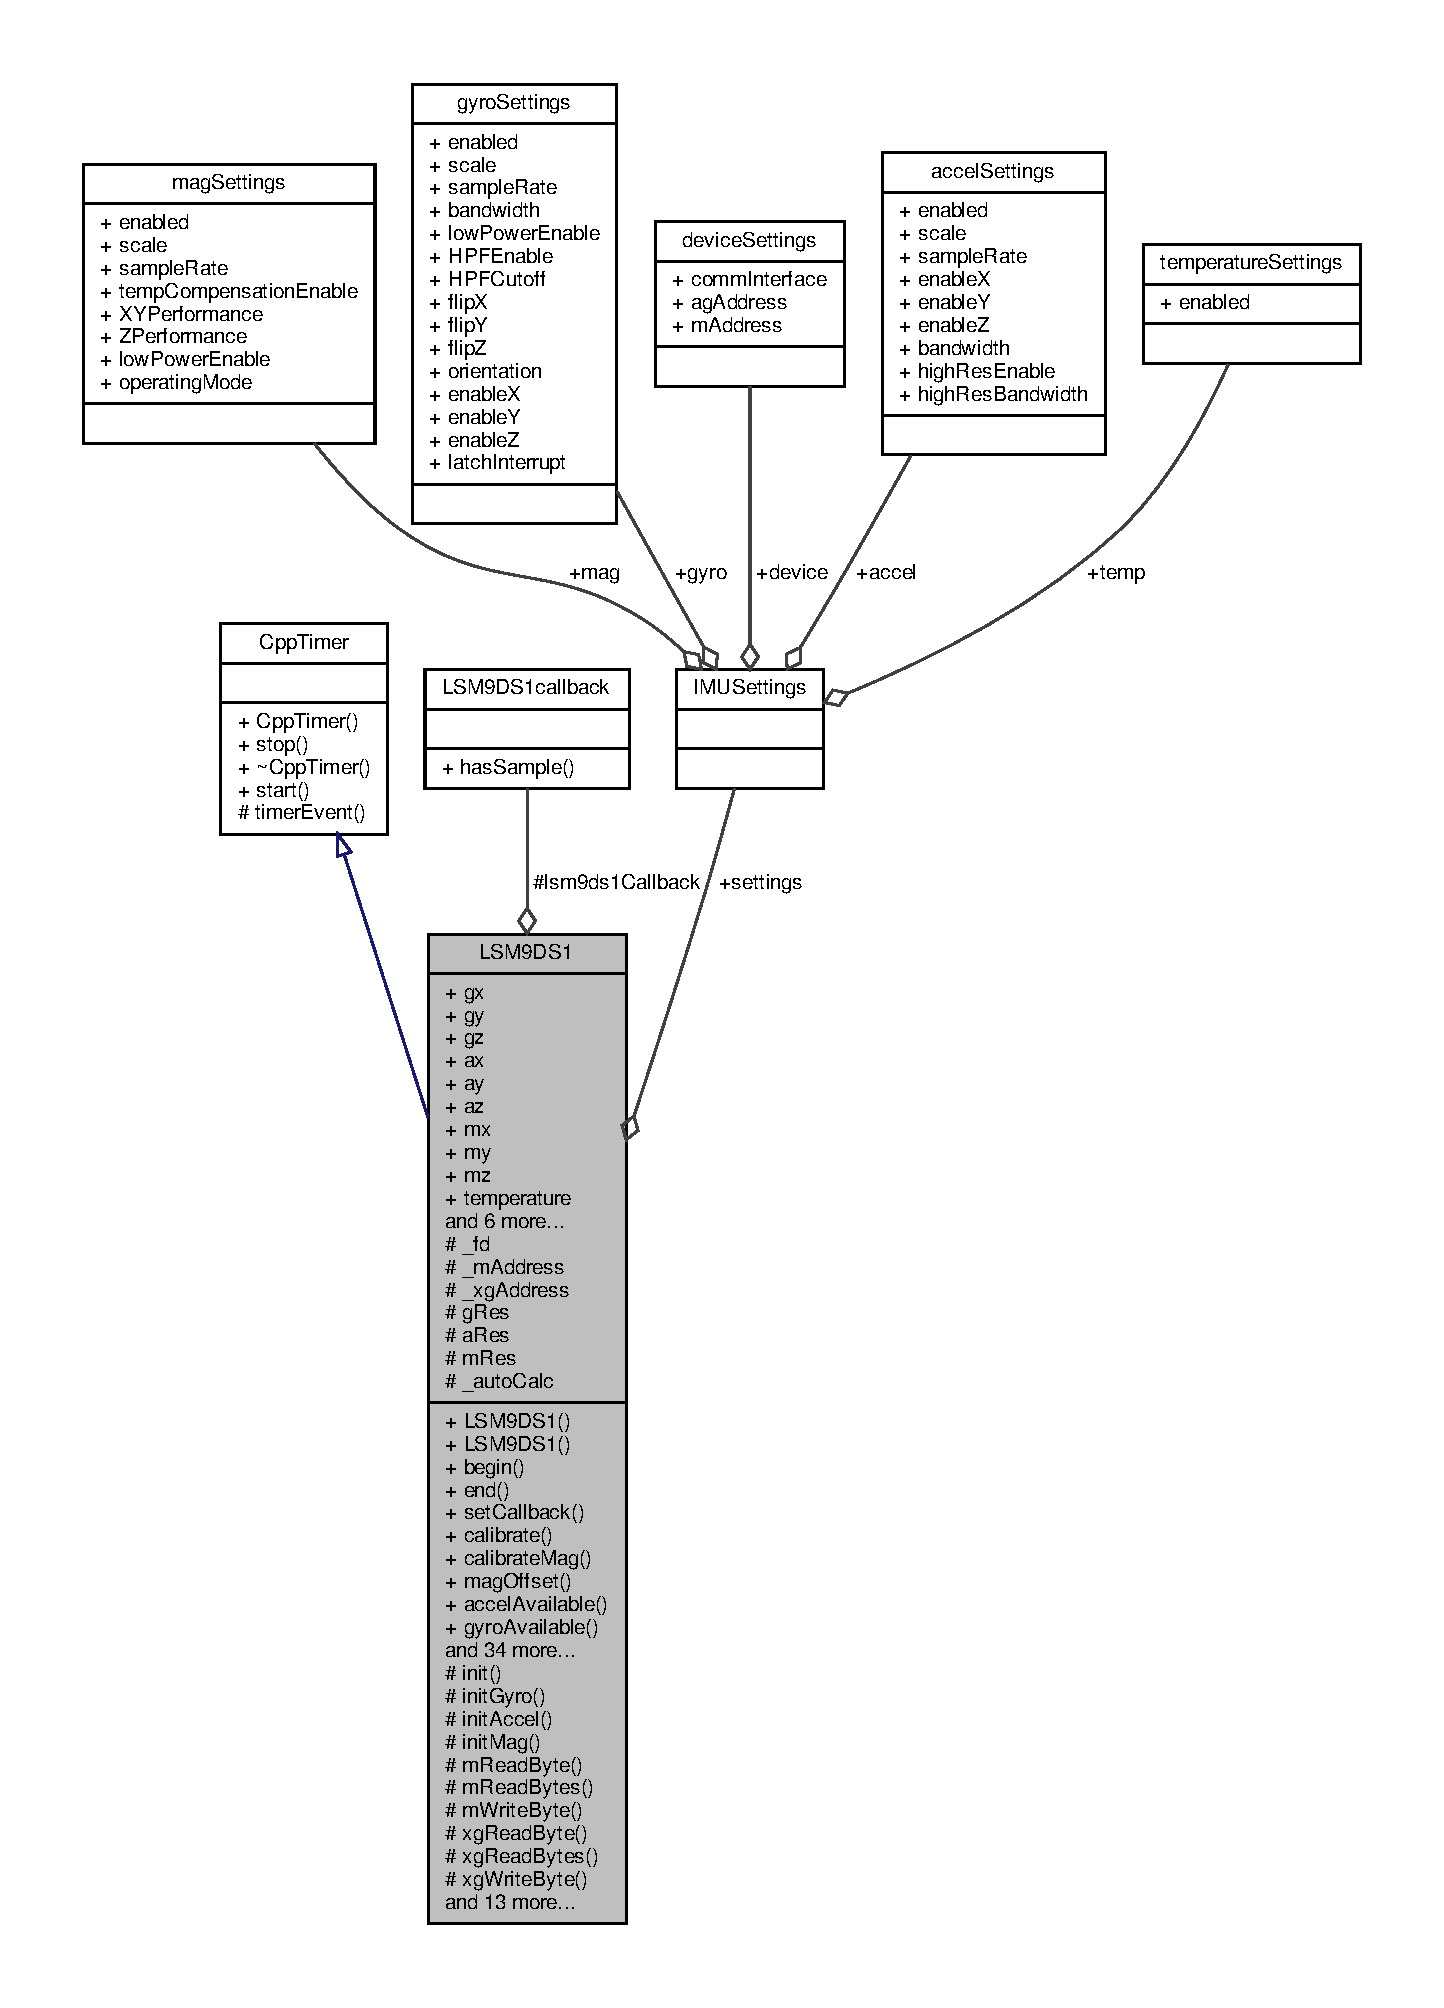
\includegraphics[width=350pt]{classLSM9DS1__coll__graph}
\end{center}
\end{figure}
\subsection*{Public Member Functions}
\begin{DoxyCompactItemize}
\item 
\hyperlink{classLSM9DS1_ab62923063ffc49dca82e6f311c5c8764}{L\+S\+M9\+D\+S1} (interface\+\_\+mode interface, uint8\+\_\+t xg\+Addr, uint8\+\_\+t m\+Addr)
\begin{DoxyCompactList}\small\item\em The Constructor. \end{DoxyCompactList}\item 
uint16\+\_\+t \hyperlink{classLSM9DS1_a8728e560c76bd120b3711af15a6ecbd6}{begin} ()
\begin{DoxyCompactList}\small\item\em Initializes the gyro, accelerometer and magnetometer. \end{DoxyCompactList}\item 
\mbox{\Hypertarget{classLSM9DS1_ae1948644d70a0356f3da4949023afb31}\label{classLSM9DS1_ae1948644d70a0356f3da4949023afb31}} 
void \hyperlink{classLSM9DS1_ae1948644d70a0356f3da4949023afb31}{end} ()
\begin{DoxyCompactList}\small\item\em Ends a possible thread in the background. \end{DoxyCompactList}\item 
void \hyperlink{classLSM9DS1_a3102ea02c253af39e3b43ee55b94d716}{set\+Callback} (\hyperlink{classLSM9DS1callback}{L\+S\+M9\+D\+S1callback} $\ast$cb)
\begin{DoxyCompactList}\small\item\em Sets a callback. \end{DoxyCompactList}\item 
void \hyperlink{classLSM9DS1_a97939cb15fcb7e33abcd6d3a9230d943}{calibrate} (bool auto\+Calc=true)
\begin{DoxyCompactList}\small\item\em Calibrates the sensor data. \end{DoxyCompactList}\item 
void \hyperlink{classLSM9DS1_afb45f0bcbcbeb15d4bd1a28821b24d14}{calibrate\+Mag} (bool load\+In=true)
\begin{DoxyCompactList}\small\item\em Calibrates the magnetometer data. \end{DoxyCompactList}\item 
void \hyperlink{classLSM9DS1_a0d461614bd058b082c94481dc916c18b}{mag\+Offset} (uint8\+\_\+t axis, int16\+\_\+t offset)
\begin{DoxyCompactList}\small\item\em Sets the magnetometer offset. \end{DoxyCompactList}\item 
uint8\+\_\+t \hyperlink{classLSM9DS1_a515ce6f5c199a86c6aa5be353b2a3a13}{accel\+Available} ()
\begin{DoxyCompactList}\small\item\em Polls the accelerometer status register to check if new data is available. \end{DoxyCompactList}\item 
uint8\+\_\+t \hyperlink{classLSM9DS1_a65b71a03a30f4e8ed1ffd46de3db0560}{gyro\+Available} ()
\begin{DoxyCompactList}\small\item\em Polls the gyroscope status register to check if new data is available. \end{DoxyCompactList}\item 
uint8\+\_\+t \hyperlink{classLSM9DS1_aaf6683c6f3f0281d5222b74f580f321b}{temp\+Available} ()
\begin{DoxyCompactList}\small\item\em Polls the temperature status register to check if new data is available. \end{DoxyCompactList}\item 
uint8\+\_\+t \hyperlink{classLSM9DS1_a85afd29e95bead7b3f0083a9a235d1df}{mag\+Available} (lsm9ds1\+\_\+axis axis=A\+L\+L\+\_\+\+A\+X\+IS)
\begin{DoxyCompactList}\small\item\em Polls the temperature status register to check if new data is available. \end{DoxyCompactList}\item 
void \hyperlink{classLSM9DS1_a56e9710cb538a4c7f7ab94c2ca256ce9}{read\+Gyro} ()
\begin{DoxyCompactList}\small\item\em Reads the gyroscope output registers. \end{DoxyCompactList}\item 
int16\+\_\+t \hyperlink{classLSM9DS1_adc1b37609a6c850328b16da4f911cefd}{read\+Gyro} (lsm9ds1\+\_\+axis axis)
\begin{DoxyCompactList}\small\item\em Reads a specific axis of the gyroscope. \end{DoxyCompactList}\item 
void \hyperlink{classLSM9DS1_a9953684a1ff652a7d3a4d91e72bccaa1}{read\+Accel} ()
\begin{DoxyCompactList}\small\item\em Reads the accelerometer output registers. \end{DoxyCompactList}\item 
int16\+\_\+t \hyperlink{classLSM9DS1_acbe3bfc0b8db7fe3f77893d22c394594}{read\+Accel} (lsm9ds1\+\_\+axis axis)
\begin{DoxyCompactList}\small\item\em Reads a specific axis of the accelerometer. \end{DoxyCompactList}\item 
void \hyperlink{classLSM9DS1_ae127cf75aa5f3c5421e49363795dcd38}{read\+Mag} ()
\begin{DoxyCompactList}\small\item\em Reads the magnetometer output registers. \end{DoxyCompactList}\item 
int16\+\_\+t \hyperlink{classLSM9DS1_a615fd3ab32a9af833ef9899663100330}{read\+Mag} (lsm9ds1\+\_\+axis axis)
\begin{DoxyCompactList}\small\item\em Reads a specific axis of the magnetometer. \end{DoxyCompactList}\item 
void \hyperlink{classLSM9DS1_aca21a51dc79a1287b97ed9c326e2080b}{read\+Temp} ()
\begin{DoxyCompactList}\small\item\em Reads the temperature output registers. \end{DoxyCompactList}\item 
float \hyperlink{classLSM9DS1_a76707323565bc4170ea8e27a932c95e4}{calc\+Gyro} (int16\+\_\+t gyro)
\begin{DoxyCompactList}\small\item\em Converts from R\+AW signed 16-\/bit value to degrees per second. \end{DoxyCompactList}\item 
float \hyperlink{classLSM9DS1_a54e2a7888b67b47cf0dd986c5b91a3c5}{calc\+Accel} (int16\+\_\+t accel)
\begin{DoxyCompactList}\small\item\em Converts from R\+AW signed 16-\/bit value to gravity (g\textquotesingle{}s). \end{DoxyCompactList}\item 
float \hyperlink{classLSM9DS1_a7d0b0740497b1a10cd3e46a282a143ec}{calc\+Mag} (int16\+\_\+t mag)
\begin{DoxyCompactList}\small\item\em Converts from R\+AW signed 16-\/bit value to Gauss (Gs). \end{DoxyCompactList}\item 
void \hyperlink{classLSM9DS1_a115d304ebcdc8c701f3e5a5d397250aa}{set\+Gyro\+Scale} (uint16\+\_\+t g\+Scl)
\begin{DoxyCompactList}\small\item\em Sets the full-\/scale range of the gyroscope. \end{DoxyCompactList}\item 
void \hyperlink{classLSM9DS1_a8656d2de1ff9cc4cb76214e4561d02c4}{set\+Accel\+Scale} (uint8\+\_\+t a\+Scl)
\begin{DoxyCompactList}\small\item\em Sets the full-\/scale range of the accelerometer. \end{DoxyCompactList}\item 
void \hyperlink{classLSM9DS1_ad7604159a07b0d088cdfb6ba4a0093b0}{set\+Mag\+Scale} (uint8\+\_\+t m\+Scl)
\begin{DoxyCompactList}\small\item\em Sets the full-\/scale range of the magnetometer. \end{DoxyCompactList}\item 
void \hyperlink{classLSM9DS1_ab8fc33c8da4fc5c379e880ff57d331fa}{set\+Gyro\+O\+DR} (uint8\+\_\+t g\+Rate)
\begin{DoxyCompactList}\small\item\em Sets the output data rate and bandwidth of the gyroscope. \end{DoxyCompactList}\item 
void \hyperlink{classLSM9DS1_a76d72839cdecc3f1c4ee6fff578182c5}{set\+Accel\+O\+DR} (uint8\+\_\+t a\+Rate)
\begin{DoxyCompactList}\small\item\em Sets the output data rate and bandwidth of the accelerometer. \end{DoxyCompactList}\item 
void \hyperlink{classLSM9DS1_a8bc672fba680edc468a643fd58046b41}{set\+Mag\+O\+DR} (uint8\+\_\+t m\+Rate)
\begin{DoxyCompactList}\small\item\em Sets the output data rate and bandwidth of the magnetometer. \end{DoxyCompactList}\item 
void \hyperlink{classLSM9DS1_a1e318c5e7c1d500c3ab2602c46265354}{config\+Inactivity} (uint8\+\_\+t duration, uint8\+\_\+t threshold, bool sleep\+On)
\begin{DoxyCompactList}\small\item\em Configures inactivity interrupt parameters. \end{DoxyCompactList}\item 
void \hyperlink{classLSM9DS1_a1e8ebc6c1e3876d8936197dc93f76717}{config\+Accel\+Int} (uint8\+\_\+t generator, bool and\+Interrupts=false)
\begin{DoxyCompactList}\small\item\em Configures Accelerometer Interrupt Generator. \end{DoxyCompactList}\item 
void \hyperlink{classLSM9DS1_acebcf64ab4e6ea7ed7a23c09ef16afe9}{config\+Accel\+Ths} (uint8\+\_\+t threshold, lsm9ds1\+\_\+axis axis, uint8\+\_\+t duration=0, bool wait=0)
\begin{DoxyCompactList}\small\item\em Configures the threshold of an accelereomter axis. \end{DoxyCompactList}\item 
void \hyperlink{classLSM9DS1_a19a341728c4e5b454de045c8a531cf06}{config\+Gyro\+Int} (uint8\+\_\+t generator, bool aoi, bool latch)
\begin{DoxyCompactList}\small\item\em Configures Gyroscope Interrupt Generator. \end{DoxyCompactList}\item 
void \hyperlink{classLSM9DS1_ad865cc972960ed476fabd54f698adf6e}{config\+Gyro\+Ths} (int16\+\_\+t threshold, lsm9ds1\+\_\+axis axis, uint8\+\_\+t duration, bool wait)
\begin{DoxyCompactList}\small\item\em Configures the threshold of a gyroscope axis. \end{DoxyCompactList}\item 
void \hyperlink{classLSM9DS1_a5b6948b9d4caf57cfe9e0559a0c7f54c}{config\+Int} (interrupt\+\_\+select interupt, uint8\+\_\+t generator, h\+\_\+lactive active\+Low=I\+N\+T\+\_\+\+A\+C\+T\+I\+V\+E\+\_\+\+L\+OW, pp\+\_\+od push\+Pull=I\+N\+T\+\_\+\+P\+U\+S\+H\+\_\+\+P\+U\+LL)
\begin{DoxyCompactList}\small\item\em Configures I\+N\+T1 or I\+N\+T2 (Gyro and Accel Interrupts only). \end{DoxyCompactList}\item 
void \hyperlink{classLSM9DS1_a54a521668eb63d504d227c6d460723e0}{config\+Mag\+Int} (uint8\+\_\+t generator, h\+\_\+lactive active\+Low, bool latch=true)
\begin{DoxyCompactList}\small\item\em Configures Magnetometer Interrupt Generator. \end{DoxyCompactList}\item 
void \hyperlink{classLSM9DS1_a87cf3dd3a4d9ca79106eb7c1c866a224}{config\+Mag\+Ths} (uint16\+\_\+t threshold)
\begin{DoxyCompactList}\small\item\em Configures the threshold of a gyroscope axis. \end{DoxyCompactList}\item 
uint8\+\_\+t \hyperlink{classLSM9DS1_aaba6696754df62a411a6a190100f9ca3}{get\+Gyro\+Int\+Src} ()
\begin{DoxyCompactList}\small\item\em Gets contents of gyroscope interrupt source register. \end{DoxyCompactList}\item 
uint8\+\_\+t \hyperlink{classLSM9DS1_ae42ae3b368370f977d090ba0e53c7f5c}{get\+Accel\+Int\+Src} ()
\begin{DoxyCompactList}\small\item\em Gets contents of accelerometer interrupt source register. \end{DoxyCompactList}\item 
uint8\+\_\+t \hyperlink{classLSM9DS1_a2bc92a37db982059b89e0a06e7d05a95}{get\+Mag\+Int\+Src} ()
\begin{DoxyCompactList}\small\item\em Gets contents of magnetometer interrupt source register. \end{DoxyCompactList}\item 
uint8\+\_\+t \hyperlink{classLSM9DS1_a9dab029d1d24e49709258d893042d28f}{get\+Inactivity} ()
\begin{DoxyCompactList}\small\item\em Gets status of inactivity interrupt. \end{DoxyCompactList}\item 
void \hyperlink{classLSM9DS1_a13b61812069b399547f177b0b0af8fe3}{sleep\+Gyro} (bool enable=true)
\begin{DoxyCompactList}\small\item\em Sets gyro to sleep or wake. \end{DoxyCompactList}\item 
void \hyperlink{classLSM9DS1_a5f01141131318697838f15d7e5d10f2c}{enable\+F\+I\+FO} (bool enable=true)
\begin{DoxyCompactList}\small\item\em Enables or disables the F\+I\+FO. \end{DoxyCompactList}\item 
void \hyperlink{classLSM9DS1_a0ec4a93a34545af1acc336bae9b360f1}{set\+F\+I\+FO} (fifo\+Mode\+\_\+type fifo\+Mode, uint8\+\_\+t fifo\+Ths)
\begin{DoxyCompactList}\small\item\em Configures F\+I\+FO mode and Threshold. \end{DoxyCompactList}\item 
uint8\+\_\+t \hyperlink{classLSM9DS1_ac03ef2ff928a25c4a80af7707cd92dc8}{get\+F\+I\+F\+O\+Samples} ()
\begin{DoxyCompactList}\small\item\em Gets number of F\+I\+FO samples. \end{DoxyCompactList}\end{DoxyCompactItemize}
\subsection*{Public Attributes}
\begin{DoxyCompactItemize}
\item 
\mbox{\Hypertarget{classLSM9DS1_a8397fc6c94a11a8a09f3dd17b28cf2a4}\label{classLSM9DS1_a8397fc6c94a11a8a09f3dd17b28cf2a4}} 
\hyperlink{structIMUSettings}{I\+M\+U\+Settings} {\bfseries settings}
\item 
\mbox{\Hypertarget{classLSM9DS1_abf02b4544b5d529036adbac02e7b9f02}\label{classLSM9DS1_abf02b4544b5d529036adbac02e7b9f02}} 
int16\+\_\+t {\bfseries gx}
\item 
\mbox{\Hypertarget{classLSM9DS1_a0c351823fd094ff24ff245dd951cf783}\label{classLSM9DS1_a0c351823fd094ff24ff245dd951cf783}} 
int16\+\_\+t {\bfseries gy}
\item 
\mbox{\Hypertarget{classLSM9DS1_ad4d0f0585398ff917afcba1b4a73e519}\label{classLSM9DS1_ad4d0f0585398ff917afcba1b4a73e519}} 
int16\+\_\+t {\bfseries gz}
\item 
\mbox{\Hypertarget{classLSM9DS1_adac13514d176cfb54aed8cda9a056335}\label{classLSM9DS1_adac13514d176cfb54aed8cda9a056335}} 
int16\+\_\+t {\bfseries ax}
\item 
\mbox{\Hypertarget{classLSM9DS1_a978a357dedfa574d6e0fad33ad71e23f}\label{classLSM9DS1_a978a357dedfa574d6e0fad33ad71e23f}} 
int16\+\_\+t {\bfseries ay}
\item 
\mbox{\Hypertarget{classLSM9DS1_aa631c8a90b90130b5be147dd4fae0841}\label{classLSM9DS1_aa631c8a90b90130b5be147dd4fae0841}} 
int16\+\_\+t {\bfseries az}
\item 
\mbox{\Hypertarget{classLSM9DS1_a0e68eb9e44969070b6d84a93ba252f71}\label{classLSM9DS1_a0e68eb9e44969070b6d84a93ba252f71}} 
int16\+\_\+t {\bfseries mx}
\item 
\mbox{\Hypertarget{classLSM9DS1_a773f80f9b7cdf8375c84a4209895d732}\label{classLSM9DS1_a773f80f9b7cdf8375c84a4209895d732}} 
int16\+\_\+t {\bfseries my}
\item 
\mbox{\Hypertarget{classLSM9DS1_aafe23993500ece9efd161e564787dce2}\label{classLSM9DS1_aafe23993500ece9efd161e564787dce2}} 
int16\+\_\+t {\bfseries mz}
\item 
\mbox{\Hypertarget{classLSM9DS1_a92791effe47c0f8c93505e53496266e5}\label{classLSM9DS1_a92791effe47c0f8c93505e53496266e5}} 
int16\+\_\+t {\bfseries temperature}
\item 
\mbox{\Hypertarget{classLSM9DS1_a8c0354ee78e029b6715ee7110bcd8753}\label{classLSM9DS1_a8c0354ee78e029b6715ee7110bcd8753}} 
float {\bfseries g\+Bias} \mbox{[}3\mbox{]}
\item 
\mbox{\Hypertarget{classLSM9DS1_abe998fcc50cfe729c13ab535337849c7}\label{classLSM9DS1_abe998fcc50cfe729c13ab535337849c7}} 
float {\bfseries a\+Bias} \mbox{[}3\mbox{]}
\item 
\mbox{\Hypertarget{classLSM9DS1_aab3753b958a1eaabfb48ffaf837dfadc}\label{classLSM9DS1_aab3753b958a1eaabfb48ffaf837dfadc}} 
float {\bfseries m\+Bias} \mbox{[}3\mbox{]}
\item 
\mbox{\Hypertarget{classLSM9DS1_ab2e59e0460cf88a12765238506031f2a}\label{classLSM9DS1_ab2e59e0460cf88a12765238506031f2a}} 
int16\+\_\+t {\bfseries g\+Bias\+Raw} \mbox{[}3\mbox{]}
\item 
\mbox{\Hypertarget{classLSM9DS1_ae42dc2f2b9f2df223c853e233191313a}\label{classLSM9DS1_ae42dc2f2b9f2df223c853e233191313a}} 
int16\+\_\+t {\bfseries a\+Bias\+Raw} \mbox{[}3\mbox{]}
\item 
\mbox{\Hypertarget{classLSM9DS1_ad0e3ab0b7eeee5378ab91dd20270a9b5}\label{classLSM9DS1_ad0e3ab0b7eeee5378ab91dd20270a9b5}} 
int16\+\_\+t {\bfseries m\+Bias\+Raw} \mbox{[}3\mbox{]}
\end{DoxyCompactItemize}
\subsection*{Protected Member Functions}
\begin{DoxyCompactItemize}
\item 
void \hyperlink{classLSM9DS1_aa4f74e09e93c0133dc30545d4492849e}{init} (interface\+\_\+mode interface, uint8\+\_\+t xg\+Addr, uint8\+\_\+t m\+Addr)
\begin{DoxyCompactList}\small\item\em Sets up gyro, accel, and mag settings to default. \end{DoxyCompactList}\item 
void \hyperlink{classLSM9DS1_a66a7b02acb28964ffc9362f25988e270}{init\+Gyro} ()
\begin{DoxyCompactList}\small\item\em Sets up the gyroscope to begin reading. \end{DoxyCompactList}\item 
void \hyperlink{classLSM9DS1_a143ff5abf4f7ba8e1c42325859106f84}{init\+Accel} ()
\begin{DoxyCompactList}\small\item\em Sets up the accelerometer to begin reading. \end{DoxyCompactList}\item 
void \hyperlink{classLSM9DS1_a492aa6edcf891f273d932636e3cc470d}{init\+Mag} ()
\begin{DoxyCompactList}\small\item\em Sets up the magnetometer to begin reading. \end{DoxyCompactList}\item 
uint8\+\_\+t \hyperlink{classLSM9DS1_ae4e470321567e4f93fc09f4cc6cd9efa}{m\+Read\+Byte} (uint8\+\_\+t sub\+Address)
\begin{DoxyCompactList}\small\item\em Reads a byte from a specified gyroscope register. \end{DoxyCompactList}\item 
void \hyperlink{classLSM9DS1_acfdf9862cad1e66c9fb61a17bfbe7477}{m\+Read\+Bytes} (uint8\+\_\+t sub\+Address, uint8\+\_\+t $\ast$dest, uint8\+\_\+t count)
\begin{DoxyCompactList}\small\item\em Reads a number of bytes -- beginning at an address and incrementing from there -- from the gyroscope. \end{DoxyCompactList}\item 
void \hyperlink{classLSM9DS1_afc171c924102c97fa1d88fa7f48bd167}{m\+Write\+Byte} (uint8\+\_\+t sub\+Address, uint8\+\_\+t data)
\begin{DoxyCompactList}\small\item\em Writes a byte to a register in the gyroscope. \end{DoxyCompactList}\item 
uint8\+\_\+t \hyperlink{classLSM9DS1_af7f9789df6f0178764c815a3380c202a}{xg\+Read\+Byte} (uint8\+\_\+t sub\+Address)
\begin{DoxyCompactList}\small\item\em Reads a byte from a register in the accel/mag sensor. \end{DoxyCompactList}\item 
void \hyperlink{classLSM9DS1_ae0a9cbfd74b1f4676f091c2d8e491d77}{xg\+Read\+Bytes} (uint8\+\_\+t sub\+Address, uint8\+\_\+t $\ast$dest, uint8\+\_\+t count)
\begin{DoxyCompactList}\small\item\em Reads a number of bytes -- beginning at an address and incrementing from there -- from the accelerometer/magnetometer. \end{DoxyCompactList}\item 
void \hyperlink{classLSM9DS1_a263eed4b52ad087a1195755c6ba49e62}{xg\+Write\+Byte} (uint8\+\_\+t sub\+Address, uint8\+\_\+t data)
\begin{DoxyCompactList}\small\item\em Writes a byte to a register in the accel/mag sensor. \end{DoxyCompactList}\item 
void \hyperlink{classLSM9DS1_a303e0dd33e000579dc3917aecedb6e63}{calcg\+Res} ()
\begin{DoxyCompactList}\small\item\em Calculates the resolution of the gyroscope. \end{DoxyCompactList}\item 
void \hyperlink{classLSM9DS1_a830dfc95c7e2d8524720d78357b053cb}{calcm\+Res} ()
\begin{DoxyCompactList}\small\item\em Calculates the resolution of the magnetometer. \end{DoxyCompactList}\item 
void \hyperlink{classLSM9DS1_a31597c9ae6c5a7de64a50cbbbcd24297}{calca\+Res} ()
\begin{DoxyCompactList}\small\item\em Calculates the resolution of the accelerometer. \end{DoxyCompactList}\item 
\mbox{\Hypertarget{classLSM9DS1_a5aadcd09cf9157de817c359e49304ca7}\label{classLSM9DS1_a5aadcd09cf9157de817c359e49304ca7}} 
void \hyperlink{classLSM9DS1_a5aadcd09cf9157de817c359e49304ca7}{constrain\+Scales} ()
\begin{DoxyCompactList}\small\item\em Constrains scales. \end{DoxyCompactList}\item 
void \hyperlink{classLSM9DS1_a4286d5803ab028c657e007ae99acc60a}{init\+S\+PI} ()
\begin{DoxyCompactList}\small\item\em Initializes the S\+PI hardware. \end{DoxyCompactList}\item 
void \hyperlink{classLSM9DS1_a83321c9d6ec50f6b9944907d2be482cd}{S\+P\+Iwrite\+Byte} (uint8\+\_\+t cs\+Pin, uint8\+\_\+t sub\+Address, uint8\+\_\+t data)
\begin{DoxyCompactList}\small\item\em Writes a byte out of S\+PI to a register in the device. \end{DoxyCompactList}\item 
uint8\+\_\+t \hyperlink{classLSM9DS1_a6f0f50bb5e9b702d5a19c7441a3f9d8b}{S\+P\+Iread\+Byte} (uint8\+\_\+t cs\+Pin, uint8\+\_\+t sub\+Address)
\begin{DoxyCompactList}\small\item\em Reads a single byte from a register over S\+PI. \end{DoxyCompactList}\item 
void \hyperlink{classLSM9DS1_a26c0f164454eba84e6486033b7061d11}{S\+P\+Iread\+Bytes} (uint8\+\_\+t cs\+Pin, uint8\+\_\+t sub\+Address, uint8\+\_\+t $\ast$dest, uint8\+\_\+t count)
\begin{DoxyCompactList}\small\item\em Initializes the S\+PI hardware. \end{DoxyCompactList}\item 
void \hyperlink{classLSM9DS1_ae60332c2836bd3f19846b7a44c015ddd}{init\+I2C} ()
\begin{DoxyCompactList}\small\item\em Initializes the I2C hardware. \end{DoxyCompactList}\item 
void \hyperlink{classLSM9DS1_a8e66108a002cc15ec4c0db0a608d20c6}{I2\+Cwrite\+Byte} (uint8\+\_\+t address, uint8\+\_\+t sub\+Address, uint8\+\_\+t data)
\begin{DoxyCompactList}\small\item\em Writes a byte out of I2C to a register in the device. \end{DoxyCompactList}\item 
uint8\+\_\+t \hyperlink{classLSM9DS1_a7fc046d4b335494331905fdeb5c81c9e}{I2\+Cread\+Byte} (uint8\+\_\+t address, uint8\+\_\+t sub\+Address)
\begin{DoxyCompactList}\small\item\em Reads a single byte from a register over I2C. \end{DoxyCompactList}\item 
uint8\+\_\+t \hyperlink{classLSM9DS1_adfc9a22290daddd7787e8023fa8f12cc}{I2\+Cread\+Bytes} (uint8\+\_\+t address, uint8\+\_\+t sub\+Address, uint8\+\_\+t $\ast$dest, uint8\+\_\+t count)
\begin{DoxyCompactList}\small\item\em Reads a series of bytes, starting at a register via S\+PI. \end{DoxyCompactList}\item 
\mbox{\Hypertarget{classLSM9DS1_ad1fffc2bc5987339430d3b293da0bdd1}\label{classLSM9DS1_ad1fffc2bc5987339430d3b293da0bdd1}} 
void \hyperlink{classLSM9DS1_ad1fffc2bc5987339430d3b293da0bdd1}{timer\+Event} ()
\begin{DoxyCompactList}\small\item\em The timer event. \end{DoxyCompactList}\end{DoxyCompactItemize}
\subsection*{Protected Attributes}
\begin{DoxyCompactItemize}
\item 
\mbox{\Hypertarget{classLSM9DS1_a8a6a3c8b294acfcf11342f602864dc42}\label{classLSM9DS1_a8a6a3c8b294acfcf11342f602864dc42}} 
int {\bfseries \+\_\+fd}
\item 
\mbox{\Hypertarget{classLSM9DS1_a7141933a2ccde95976e4eecd598ecb17}\label{classLSM9DS1_a7141933a2ccde95976e4eecd598ecb17}} 
uint8\+\_\+t {\bfseries \+\_\+m\+Address}
\item 
\mbox{\Hypertarget{classLSM9DS1_ac78b7fab605570a16433a4636f91451e}\label{classLSM9DS1_ac78b7fab605570a16433a4636f91451e}} 
uint8\+\_\+t {\bfseries \+\_\+xg\+Address}
\item 
\mbox{\Hypertarget{classLSM9DS1_a2d8654ebb35177088a67e67a944bd998}\label{classLSM9DS1_a2d8654ebb35177088a67e67a944bd998}} 
float {\bfseries g\+Res}
\item 
\mbox{\Hypertarget{classLSM9DS1_acdc1f9b300b3c349e17dd21c9bb37c40}\label{classLSM9DS1_acdc1f9b300b3c349e17dd21c9bb37c40}} 
float {\bfseries a\+Res}
\item 
\mbox{\Hypertarget{classLSM9DS1_aac7ae43adf399e8052464b966aec8472}\label{classLSM9DS1_aac7ae43adf399e8052464b966aec8472}} 
float {\bfseries m\+Res}
\item 
\mbox{\Hypertarget{classLSM9DS1_a8460d00ea0bb496c5d49190a34e54588}\label{classLSM9DS1_a8460d00ea0bb496c5d49190a34e54588}} 
bool {\bfseries \+\_\+auto\+Calc}
\item 
\mbox{\Hypertarget{classLSM9DS1_aa2be4bac7f3b70c3fb11126e06a240b4}\label{classLSM9DS1_aa2be4bac7f3b70c3fb11126e06a240b4}} 
\hyperlink{classLSM9DS1callback}{L\+S\+M9\+D\+S1callback} $\ast$ {\bfseries lsm9ds1\+Callback} = N\+U\+LL
\end{DoxyCompactItemize}


\subsection{Detailed Description}
Class to enable sensor readings. 

\subsection{Constructor \& Destructor Documentation}
\mbox{\Hypertarget{classLSM9DS1_ab62923063ffc49dca82e6f311c5c8764}\label{classLSM9DS1_ab62923063ffc49dca82e6f311c5c8764}} 
\index{L\+S\+M9\+D\+S1@{L\+S\+M9\+D\+S1}!L\+S\+M9\+D\+S1@{L\+S\+M9\+D\+S1}}
\index{L\+S\+M9\+D\+S1@{L\+S\+M9\+D\+S1}!L\+S\+M9\+D\+S1@{L\+S\+M9\+D\+S1}}
\subsubsection{\texorpdfstring{L\+S\+M9\+D\+S1()}{LSM9DS1()}}
{\footnotesize\ttfamily L\+S\+M9\+D\+S1\+::\+L\+S\+M9\+D\+S1 (\begin{DoxyParamCaption}\item[{interface\+\_\+mode}]{interface,  }\item[{uint8\+\_\+t}]{xg\+Addr,  }\item[{uint8\+\_\+t}]{m\+Addr }\end{DoxyParamCaption})}



The Constructor. 

The constructor sets up private variables and sets the communication mode.


\begin{DoxyParams}{Parameters}
{\em interface} & sets the interface, either I\+M\+U\+\_\+\+M\+O\+D\+E\+\_\+\+S\+PI or I\+M\+U\+\_\+\+M\+O\+D\+E\+\_\+\+I2C \\
\hline
{\em xg\+Addr} & sets an address or pin. If M\+U\+\_\+\+M\+O\+D\+E\+\_\+\+I2C, this is the I2C address of the accel/gyroscope and if I\+M\+U\+\_\+\+M\+O\+D\+E\+\_\+\+S\+PI, this is the chip select pin of the gyro (C\+S\+\_\+\+AG). \\
\hline
{\em m\+Addr} & sets an address or pin. If I\+M\+U\+\_\+\+M\+O\+D\+E\+\_\+\+I2C, this is the I2C address of the magnetometer and if I\+M\+U\+\_\+\+M\+O\+D\+E\+\_\+\+S\+PI, this is the cs pin of the magnetometer (C\+S\+\_\+M). \\
\hline
\end{DoxyParams}
Here is the call graph for this function\+:\nopagebreak
\begin{figure}[H]
\begin{center}
\leavevmode
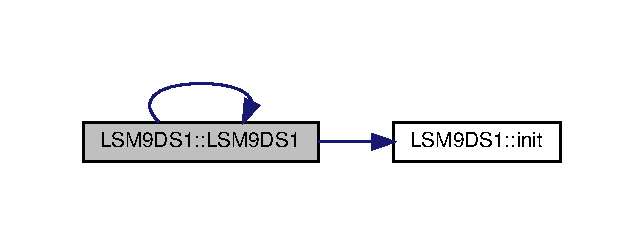
\includegraphics[width=309pt]{classLSM9DS1_ab62923063ffc49dca82e6f311c5c8764_cgraph}
\end{center}
\end{figure}
Here is the caller graph for this function\+:\nopagebreak
\begin{figure}[H]
\begin{center}
\leavevmode
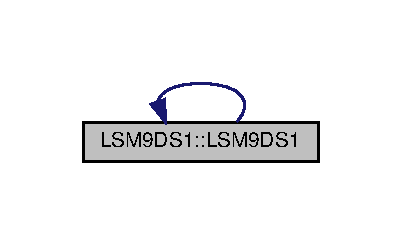
\includegraphics[width=193pt]{classLSM9DS1_ab62923063ffc49dca82e6f311c5c8764_icgraph}
\end{center}
\end{figure}


\subsection{Member Function Documentation}
\mbox{\Hypertarget{classLSM9DS1_a515ce6f5c199a86c6aa5be353b2a3a13}\label{classLSM9DS1_a515ce6f5c199a86c6aa5be353b2a3a13}} 
\index{L\+S\+M9\+D\+S1@{L\+S\+M9\+D\+S1}!accel\+Available@{accel\+Available}}
\index{accel\+Available@{accel\+Available}!L\+S\+M9\+D\+S1@{L\+S\+M9\+D\+S1}}
\subsubsection{\texorpdfstring{accel\+Available()}{accelAvailable()}}
{\footnotesize\ttfamily uint8\+\_\+t L\+S\+M9\+D\+S1\+::accel\+Available (\begin{DoxyParamCaption}{ }\end{DoxyParamCaption})}



Polls the accelerometer status register to check if new data is available. 

\begin{DoxyReturn}{Returns}
1 if new data is available, 0 if no new data is available. 
\end{DoxyReturn}
Here is the call graph for this function\+:\nopagebreak
\begin{figure}[H]
\begin{center}
\leavevmode
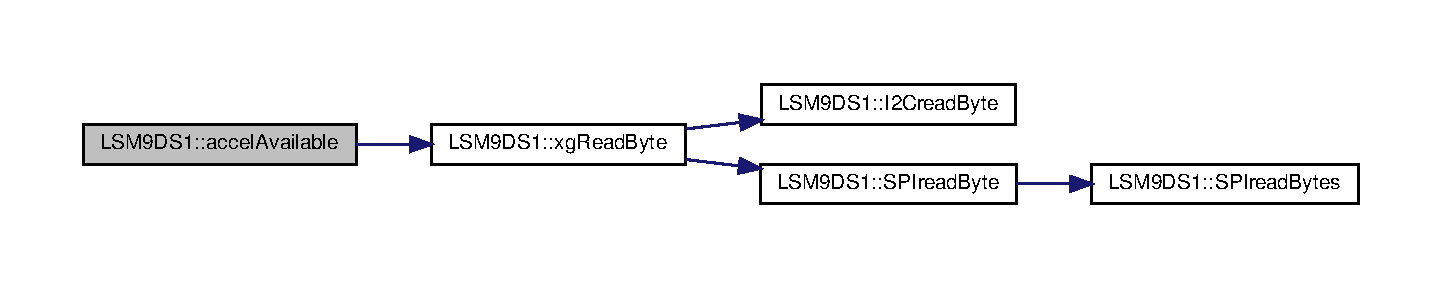
\includegraphics[width=350pt]{classLSM9DS1_a515ce6f5c199a86c6aa5be353b2a3a13_cgraph}
\end{center}
\end{figure}
\mbox{\Hypertarget{classLSM9DS1_a8728e560c76bd120b3711af15a6ecbd6}\label{classLSM9DS1_a8728e560c76bd120b3711af15a6ecbd6}} 
\index{L\+S\+M9\+D\+S1@{L\+S\+M9\+D\+S1}!begin@{begin}}
\index{begin@{begin}!L\+S\+M9\+D\+S1@{L\+S\+M9\+D\+S1}}
\subsubsection{\texorpdfstring{begin()}{begin()}}
{\footnotesize\ttfamily uint16\+\_\+t L\+S\+M9\+D\+S1\+::begin (\begin{DoxyParamCaption}{ }\end{DoxyParamCaption})}



Initializes the gyro, accelerometer and magnetometer. 

This will set up the scale and output rate of each sensor. The values set in the \hyperlink{structIMUSettings}{I\+M\+U\+Settings} struct will take effect after calling this function.

\begin{DoxyReturn}{Returns}
who\+Am\+I\+Combined. 
\end{DoxyReturn}
Todo\+: don\textquotesingle{}t use \+\_\+xg\+Address or \+\_\+m\+Address, duplicating memory Here is the call graph for this function\+:\nopagebreak
\begin{figure}[H]
\begin{center}
\leavevmode
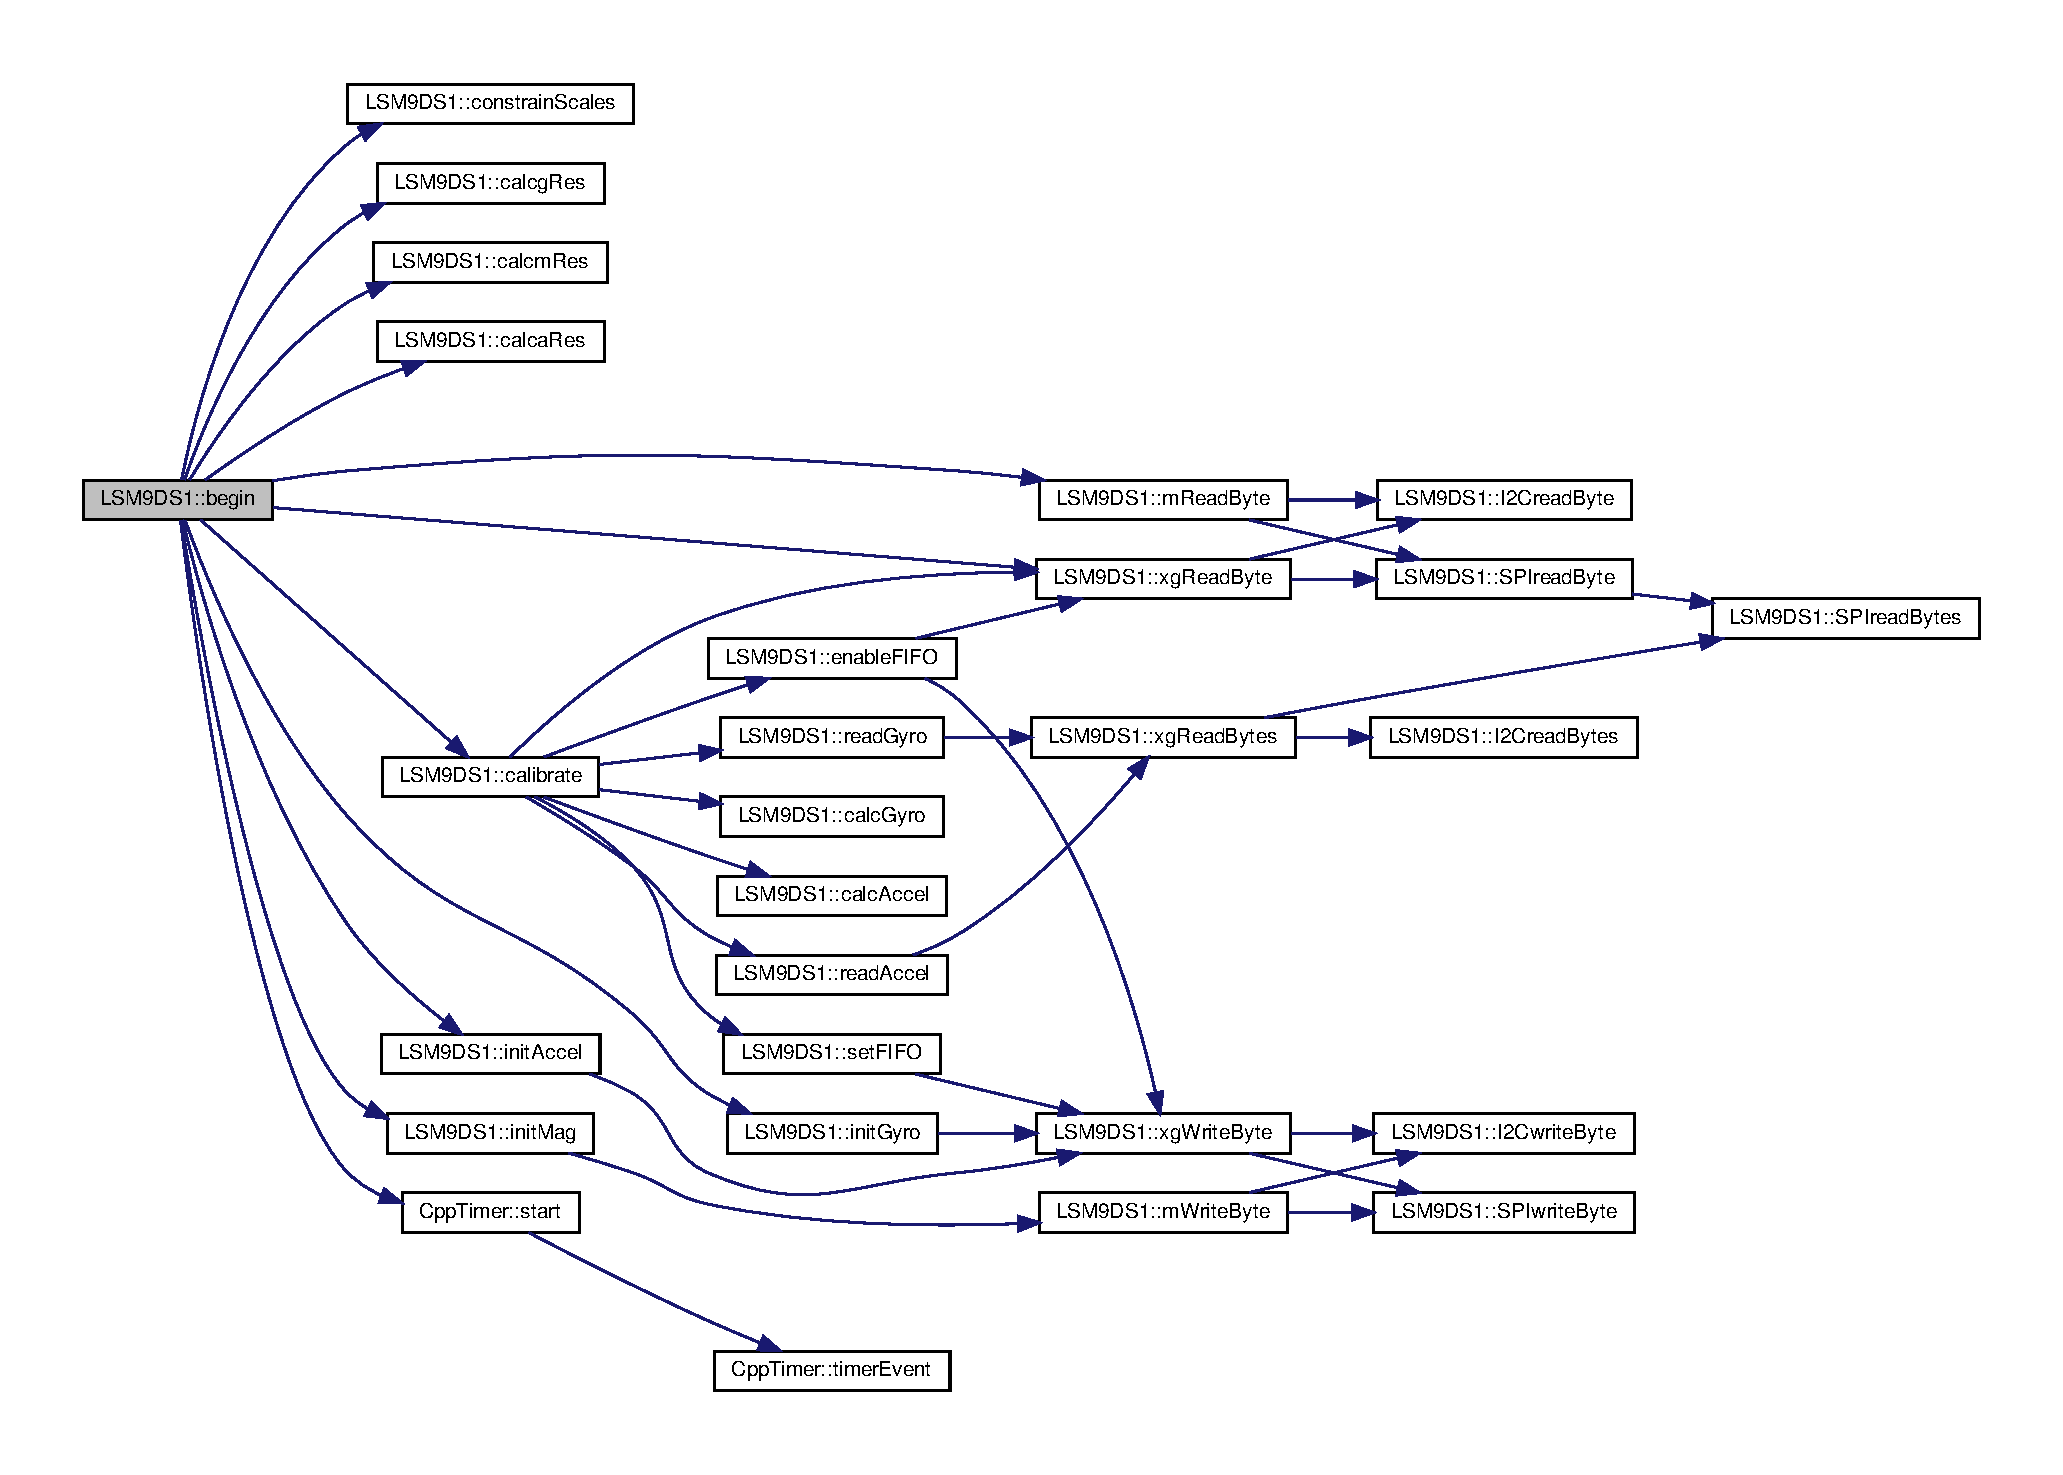
\includegraphics[width=350pt]{classLSM9DS1_a8728e560c76bd120b3711af15a6ecbd6_cgraph}
\end{center}
\end{figure}
\mbox{\Hypertarget{classLSM9DS1_a54e2a7888b67b47cf0dd986c5b91a3c5}\label{classLSM9DS1_a54e2a7888b67b47cf0dd986c5b91a3c5}} 
\index{L\+S\+M9\+D\+S1@{L\+S\+M9\+D\+S1}!calc\+Accel@{calc\+Accel}}
\index{calc\+Accel@{calc\+Accel}!L\+S\+M9\+D\+S1@{L\+S\+M9\+D\+S1}}
\subsubsection{\texorpdfstring{calc\+Accel()}{calcAccel()}}
{\footnotesize\ttfamily float L\+S\+M9\+D\+S1\+::calc\+Accel (\begin{DoxyParamCaption}\item[{int16\+\_\+t}]{accel }\end{DoxyParamCaption})}



Converts from R\+AW signed 16-\/bit value to gravity (g\textquotesingle{}s). 

This function reads in a signed 16-\/bit value and returns the scaled g\textquotesingle{}s. This function relies on a\+Scale and a\+Res being correct.


\begin{DoxyParams}{Parameters}
{\em accel} & is a signed 16-\/bit raw reading from the accelerometer. \\
\hline
\end{DoxyParams}
\begin{DoxyReturn}{Returns}
the accel raw reading times our pre-\/calculated g\textquotesingle{}s / (A\+DC tick). 
\end{DoxyReturn}
Here is the caller graph for this function\+:\nopagebreak
\begin{figure}[H]
\begin{center}
\leavevmode
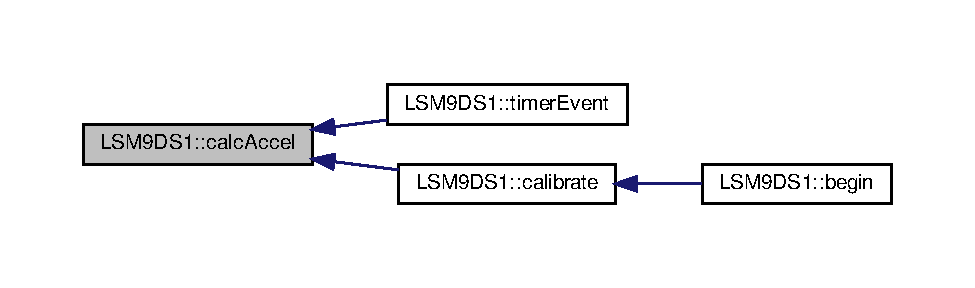
\includegraphics[width=350pt]{classLSM9DS1_a54e2a7888b67b47cf0dd986c5b91a3c5_icgraph}
\end{center}
\end{figure}
\mbox{\Hypertarget{classLSM9DS1_a31597c9ae6c5a7de64a50cbbbcd24297}\label{classLSM9DS1_a31597c9ae6c5a7de64a50cbbbcd24297}} 
\index{L\+S\+M9\+D\+S1@{L\+S\+M9\+D\+S1}!calca\+Res@{calca\+Res}}
\index{calca\+Res@{calca\+Res}!L\+S\+M9\+D\+S1@{L\+S\+M9\+D\+S1}}
\subsubsection{\texorpdfstring{calca\+Res()}{calcaRes()}}
{\footnotesize\ttfamily void L\+S\+M9\+D\+S1\+::calca\+Res (\begin{DoxyParamCaption}{ }\end{DoxyParamCaption})\hspace{0.3cm}{\ttfamily [protected]}}



Calculates the resolution of the accelerometer. 

This function will set the value of the a\+Res variable. a\+Scale must be set prior to calling this function. Here is the caller graph for this function\+:\nopagebreak
\begin{figure}[H]
\begin{center}
\leavevmode
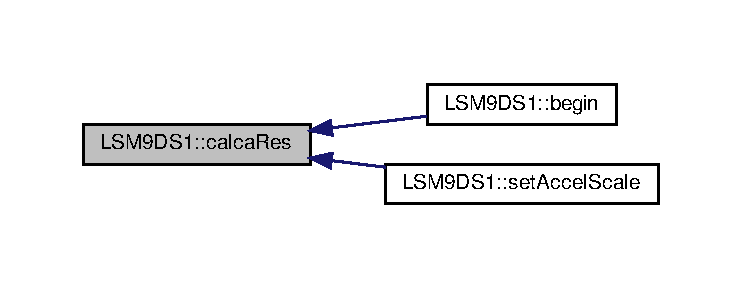
\includegraphics[width=350pt]{classLSM9DS1_a31597c9ae6c5a7de64a50cbbbcd24297_icgraph}
\end{center}
\end{figure}
\mbox{\Hypertarget{classLSM9DS1_a303e0dd33e000579dc3917aecedb6e63}\label{classLSM9DS1_a303e0dd33e000579dc3917aecedb6e63}} 
\index{L\+S\+M9\+D\+S1@{L\+S\+M9\+D\+S1}!calcg\+Res@{calcg\+Res}}
\index{calcg\+Res@{calcg\+Res}!L\+S\+M9\+D\+S1@{L\+S\+M9\+D\+S1}}
\subsubsection{\texorpdfstring{calcg\+Res()}{calcgRes()}}
{\footnotesize\ttfamily void L\+S\+M9\+D\+S1\+::calcg\+Res (\begin{DoxyParamCaption}{ }\end{DoxyParamCaption})\hspace{0.3cm}{\ttfamily [protected]}}



Calculates the resolution of the gyroscope. 

This function will set the value of the g\+Res variable. g\+Scale must be set prior to calling this function. Here is the caller graph for this function\+:\nopagebreak
\begin{figure}[H]
\begin{center}
\leavevmode
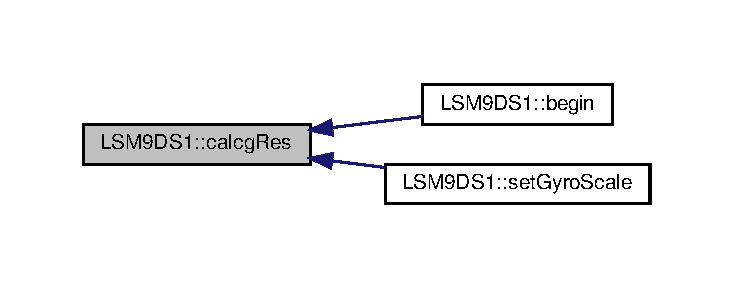
\includegraphics[width=350pt]{classLSM9DS1_a303e0dd33e000579dc3917aecedb6e63_icgraph}
\end{center}
\end{figure}
\mbox{\Hypertarget{classLSM9DS1_a76707323565bc4170ea8e27a932c95e4}\label{classLSM9DS1_a76707323565bc4170ea8e27a932c95e4}} 
\index{L\+S\+M9\+D\+S1@{L\+S\+M9\+D\+S1}!calc\+Gyro@{calc\+Gyro}}
\index{calc\+Gyro@{calc\+Gyro}!L\+S\+M9\+D\+S1@{L\+S\+M9\+D\+S1}}
\subsubsection{\texorpdfstring{calc\+Gyro()}{calcGyro()}}
{\footnotesize\ttfamily float L\+S\+M9\+D\+S1\+::calc\+Gyro (\begin{DoxyParamCaption}\item[{int16\+\_\+t}]{gyro }\end{DoxyParamCaption})}



Converts from R\+AW signed 16-\/bit value to degrees per second. 

This function reads in a signed 16-\/bit value and returns the scaled D\+PS. This function relies on g\+Scale and g\+Res being correct.


\begin{DoxyParams}{Parameters}
{\em gyro} & is a signed 16-\/bit raw reading from the gyroscope. \\
\hline
\end{DoxyParams}
\begin{DoxyReturn}{Returns}
the gyro raw reading times our pre-\/calculated D\+PS / (A\+DC tick). 
\end{DoxyReturn}
Here is the caller graph for this function\+:\nopagebreak
\begin{figure}[H]
\begin{center}
\leavevmode
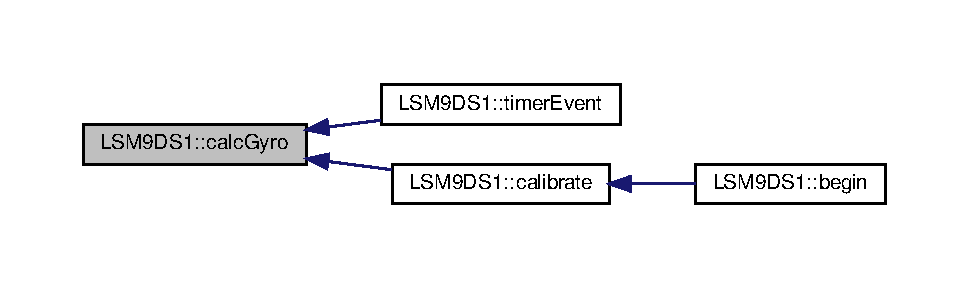
\includegraphics[width=350pt]{classLSM9DS1_a76707323565bc4170ea8e27a932c95e4_icgraph}
\end{center}
\end{figure}
\mbox{\Hypertarget{classLSM9DS1_a7d0b0740497b1a10cd3e46a282a143ec}\label{classLSM9DS1_a7d0b0740497b1a10cd3e46a282a143ec}} 
\index{L\+S\+M9\+D\+S1@{L\+S\+M9\+D\+S1}!calc\+Mag@{calc\+Mag}}
\index{calc\+Mag@{calc\+Mag}!L\+S\+M9\+D\+S1@{L\+S\+M9\+D\+S1}}
\subsubsection{\texorpdfstring{calc\+Mag()}{calcMag()}}
{\footnotesize\ttfamily float L\+S\+M9\+D\+S1\+::calc\+Mag (\begin{DoxyParamCaption}\item[{int16\+\_\+t}]{mag }\end{DoxyParamCaption})}



Converts from R\+AW signed 16-\/bit value to Gauss (Gs). 

This function reads in a signed 16-\/bit value and returns the scaled Gs. This function relies on m\+Scale and m\+Res being correct.


\begin{DoxyParams}{Parameters}
{\em mag} & is a signed 16-\/bit raw reading from the magnetometer. \\
\hline
\end{DoxyParams}
\begin{DoxyReturn}{Returns}
the mag raw reading times our pre-\/calculated Gs / (A\+DC tick). 
\end{DoxyReturn}
Here is the caller graph for this function\+:\nopagebreak
\begin{figure}[H]
\begin{center}
\leavevmode
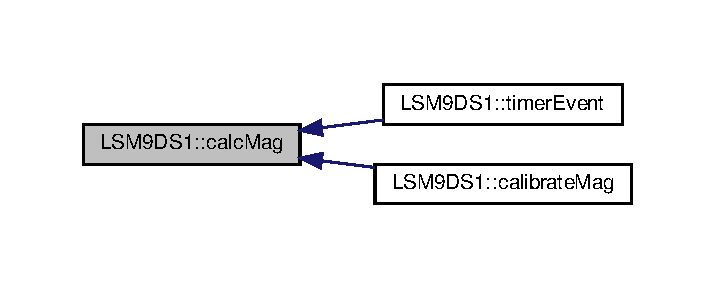
\includegraphics[width=343pt]{classLSM9DS1_a7d0b0740497b1a10cd3e46a282a143ec_icgraph}
\end{center}
\end{figure}
\mbox{\Hypertarget{classLSM9DS1_a830dfc95c7e2d8524720d78357b053cb}\label{classLSM9DS1_a830dfc95c7e2d8524720d78357b053cb}} 
\index{L\+S\+M9\+D\+S1@{L\+S\+M9\+D\+S1}!calcm\+Res@{calcm\+Res}}
\index{calcm\+Res@{calcm\+Res}!L\+S\+M9\+D\+S1@{L\+S\+M9\+D\+S1}}
\subsubsection{\texorpdfstring{calcm\+Res()}{calcmRes()}}
{\footnotesize\ttfamily void L\+S\+M9\+D\+S1\+::calcm\+Res (\begin{DoxyParamCaption}{ }\end{DoxyParamCaption})\hspace{0.3cm}{\ttfamily [protected]}}



Calculates the resolution of the magnetometer. 

This function will set the value of the m\+Res variable. m\+Scale must be set prior to calling this function. Here is the caller graph for this function\+:\nopagebreak
\begin{figure}[H]
\begin{center}
\leavevmode
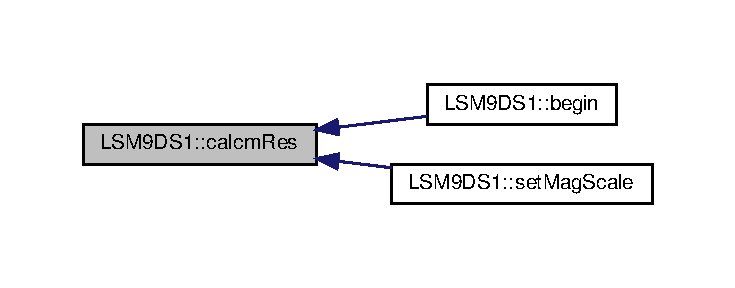
\includegraphics[width=350pt]{classLSM9DS1_a830dfc95c7e2d8524720d78357b053cb_icgraph}
\end{center}
\end{figure}
\mbox{\Hypertarget{classLSM9DS1_a97939cb15fcb7e33abcd6d3a9230d943}\label{classLSM9DS1_a97939cb15fcb7e33abcd6d3a9230d943}} 
\index{L\+S\+M9\+D\+S1@{L\+S\+M9\+D\+S1}!calibrate@{calibrate}}
\index{calibrate@{calibrate}!L\+S\+M9\+D\+S1@{L\+S\+M9\+D\+S1}}
\subsubsection{\texorpdfstring{calibrate()}{calibrate()}}
{\footnotesize\ttfamily void L\+S\+M9\+D\+S1\+::calibrate (\begin{DoxyParamCaption}\item[{bool}]{auto\+Calc = {\ttfamily true} }\end{DoxyParamCaption})}



Calibrates the sensor data. 


\begin{DoxyParams}{Parameters}
{\em auto\+Calc} & could either be set true (default) or false. \\
\hline
\end{DoxyParams}
Here is the call graph for this function\+:\nopagebreak
\begin{figure}[H]
\begin{center}
\leavevmode
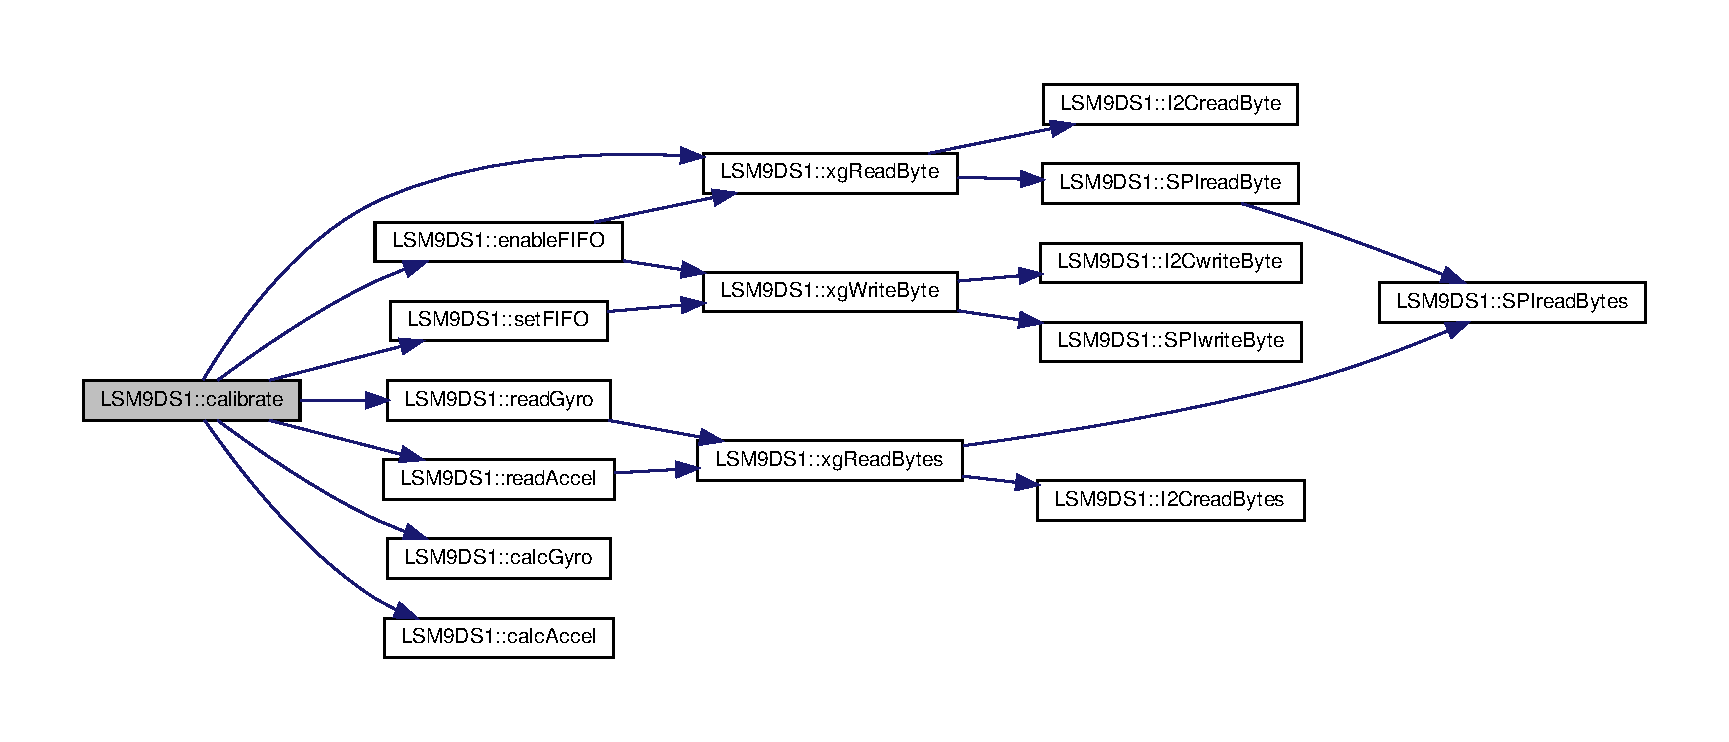
\includegraphics[width=350pt]{classLSM9DS1_a97939cb15fcb7e33abcd6d3a9230d943_cgraph}
\end{center}
\end{figure}
Here is the caller graph for this function\+:\nopagebreak
\begin{figure}[H]
\begin{center}
\leavevmode
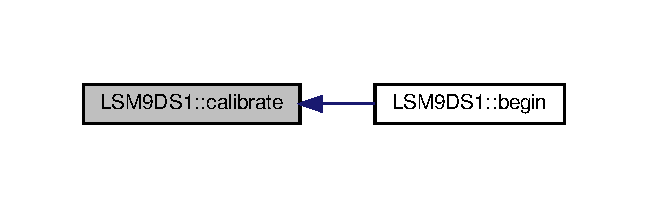
\includegraphics[width=311pt]{classLSM9DS1_a97939cb15fcb7e33abcd6d3a9230d943_icgraph}
\end{center}
\end{figure}
\mbox{\Hypertarget{classLSM9DS1_afb45f0bcbcbeb15d4bd1a28821b24d14}\label{classLSM9DS1_afb45f0bcbcbeb15d4bd1a28821b24d14}} 
\index{L\+S\+M9\+D\+S1@{L\+S\+M9\+D\+S1}!calibrate\+Mag@{calibrate\+Mag}}
\index{calibrate\+Mag@{calibrate\+Mag}!L\+S\+M9\+D\+S1@{L\+S\+M9\+D\+S1}}
\subsubsection{\texorpdfstring{calibrate\+Mag()}{calibrateMag()}}
{\footnotesize\ttfamily void L\+S\+M9\+D\+S1\+::calibrate\+Mag (\begin{DoxyParamCaption}\item[{bool}]{load\+In = {\ttfamily true} }\end{DoxyParamCaption})}



Calibrates the magnetometer data. 


\begin{DoxyParams}{Parameters}
{\em auto\+Calc} & could either be set true (default) or false. \\
\hline
\end{DoxyParams}
Here is the call graph for this function\+:\nopagebreak
\begin{figure}[H]
\begin{center}
\leavevmode
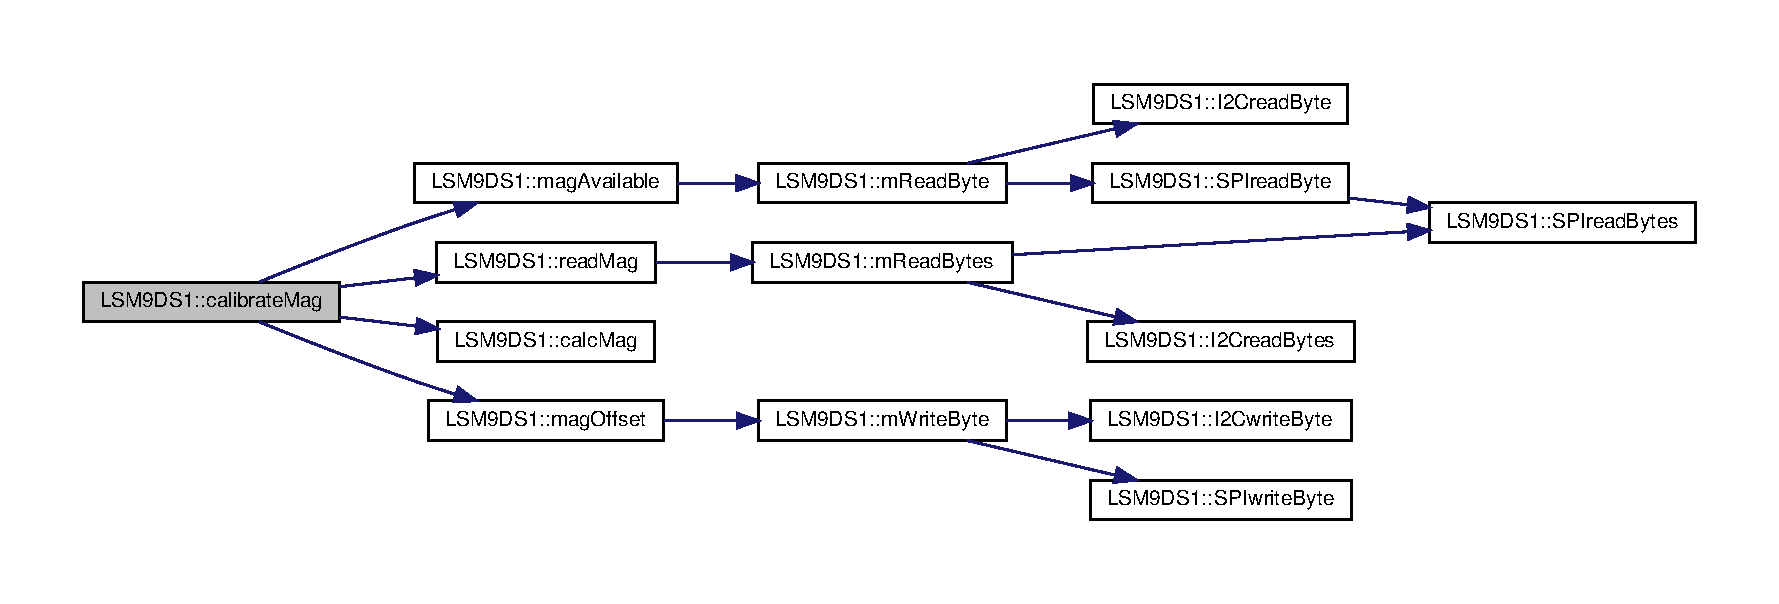
\includegraphics[width=350pt]{classLSM9DS1_afb45f0bcbcbeb15d4bd1a28821b24d14_cgraph}
\end{center}
\end{figure}
\mbox{\Hypertarget{classLSM9DS1_a1e8ebc6c1e3876d8936197dc93f76717}\label{classLSM9DS1_a1e8ebc6c1e3876d8936197dc93f76717}} 
\index{L\+S\+M9\+D\+S1@{L\+S\+M9\+D\+S1}!config\+Accel\+Int@{config\+Accel\+Int}}
\index{config\+Accel\+Int@{config\+Accel\+Int}!L\+S\+M9\+D\+S1@{L\+S\+M9\+D\+S1}}
\subsubsection{\texorpdfstring{config\+Accel\+Int()}{configAccelInt()}}
{\footnotesize\ttfamily void L\+S\+M9\+D\+S1\+::config\+Accel\+Int (\begin{DoxyParamCaption}\item[{uint8\+\_\+t}]{generator,  }\item[{bool}]{and\+Interrupts = {\ttfamily false} }\end{DoxyParamCaption})}



Configures Accelerometer Interrupt Generator. 


\begin{DoxyParams}{Parameters}
{\em generator} & is the interrupt axis/high-\/low events. Any OR\textquotesingle{}d combination of Z\+H\+I\+E\+\_\+\+XL, Z\+L\+I\+E\+\_\+\+XL, Y\+H\+I\+E\+\_\+\+XL, Y\+L\+I\+E\+\_\+\+XL, X\+H\+I\+E\+\_\+\+XL, X\+L\+I\+E\+\_\+\+XL \\
\hline
{\em and\+Interrupts} & A\+N\+D/\+OR combination of interrupt events. true\+: A\+ND combination false\+: OR combination \\
\hline
\end{DoxyParams}
Here is the call graph for this function\+:\nopagebreak
\begin{figure}[H]
\begin{center}
\leavevmode
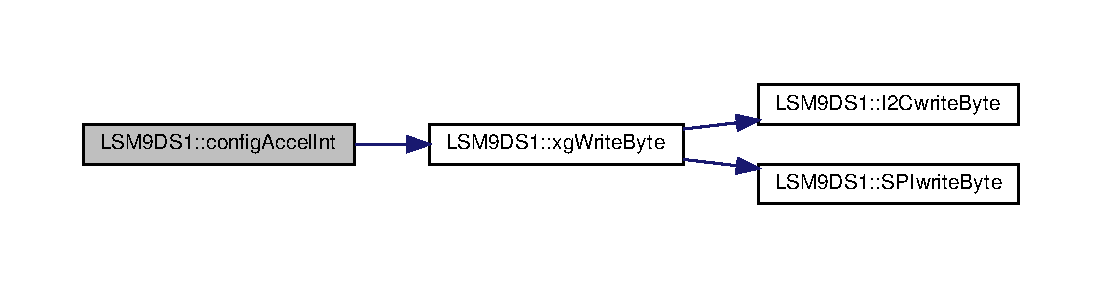
\includegraphics[width=350pt]{classLSM9DS1_a1e8ebc6c1e3876d8936197dc93f76717_cgraph}
\end{center}
\end{figure}
\mbox{\Hypertarget{classLSM9DS1_acebcf64ab4e6ea7ed7a23c09ef16afe9}\label{classLSM9DS1_acebcf64ab4e6ea7ed7a23c09ef16afe9}} 
\index{L\+S\+M9\+D\+S1@{L\+S\+M9\+D\+S1}!config\+Accel\+Ths@{config\+Accel\+Ths}}
\index{config\+Accel\+Ths@{config\+Accel\+Ths}!L\+S\+M9\+D\+S1@{L\+S\+M9\+D\+S1}}
\subsubsection{\texorpdfstring{config\+Accel\+Ths()}{configAccelThs()}}
{\footnotesize\ttfamily void L\+S\+M9\+D\+S1\+::config\+Accel\+Ths (\begin{DoxyParamCaption}\item[{uint8\+\_\+t}]{threshold,  }\item[{lsm9ds1\+\_\+axis}]{axis,  }\item[{uint8\+\_\+t}]{duration = {\ttfamily 0},  }\item[{bool}]{wait = {\ttfamily 0} }\end{DoxyParamCaption})}



Configures the threshold of an accelereomter axis. 


\begin{DoxyParams}{Parameters}
{\em threshold} & is the interrupt threshold. Possible values\+: 0-\/255. \\
\hline
{\em axis} & the axis to be configured. Either X\+\_\+\+A\+X\+IS, Y\+\_\+\+A\+X\+IS, or Z\+\_\+\+A\+X\+IS. \\
\hline
{\em duration} & the value must be above or below threshold to trigger intrerrupt. \\
\hline
{\em wait} & the duration samples before exiting the interrupt. true\+: Wait for duration samples before exiting interrupt false\+: Wait function off \\
\hline
\end{DoxyParams}
Here is the call graph for this function\+:\nopagebreak
\begin{figure}[H]
\begin{center}
\leavevmode
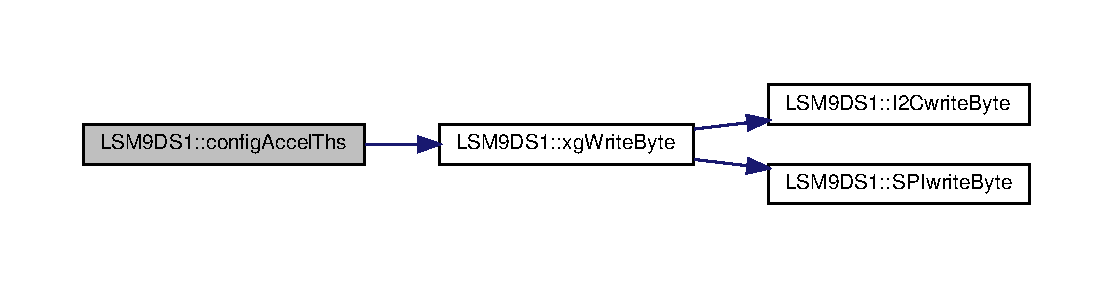
\includegraphics[width=350pt]{classLSM9DS1_acebcf64ab4e6ea7ed7a23c09ef16afe9_cgraph}
\end{center}
\end{figure}
\mbox{\Hypertarget{classLSM9DS1_a19a341728c4e5b454de045c8a531cf06}\label{classLSM9DS1_a19a341728c4e5b454de045c8a531cf06}} 
\index{L\+S\+M9\+D\+S1@{L\+S\+M9\+D\+S1}!config\+Gyro\+Int@{config\+Gyro\+Int}}
\index{config\+Gyro\+Int@{config\+Gyro\+Int}!L\+S\+M9\+D\+S1@{L\+S\+M9\+D\+S1}}
\subsubsection{\texorpdfstring{config\+Gyro\+Int()}{configGyroInt()}}
{\footnotesize\ttfamily void L\+S\+M9\+D\+S1\+::config\+Gyro\+Int (\begin{DoxyParamCaption}\item[{uint8\+\_\+t}]{generator,  }\item[{bool}]{aoi,  }\item[{bool}]{latch }\end{DoxyParamCaption})}



Configures Gyroscope Interrupt Generator. 


\begin{DoxyParams}{Parameters}
{\em generator} & interrupts axis/high-\/low events. Any OR\textquotesingle{}d combination of Z\+H\+I\+E\+\_\+G, Z\+L\+I\+E\+\_\+G, Y\+H\+I\+E\+\_\+G, Y\+L\+I\+E\+\_\+G, X\+H\+I\+E\+\_\+G, X\+L\+I\+E\+\_\+G \\
\hline
{\em aoi} & A\+N\+D/\+OR combination of interrupt events. true\+: A\+ND combination false\+: OR combination \\
\hline
{\em latch} & latches gyroscope interrupt request. \\
\hline
\end{DoxyParams}
Here is the call graph for this function\+:\nopagebreak
\begin{figure}[H]
\begin{center}
\leavevmode
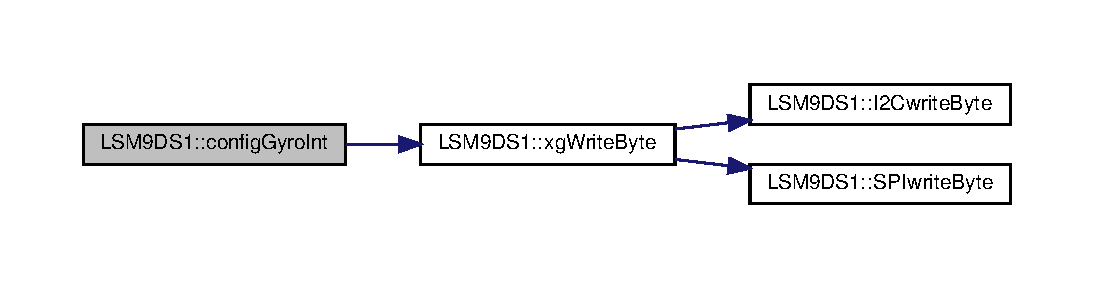
\includegraphics[width=350pt]{classLSM9DS1_a19a341728c4e5b454de045c8a531cf06_cgraph}
\end{center}
\end{figure}
\mbox{\Hypertarget{classLSM9DS1_ad865cc972960ed476fabd54f698adf6e}\label{classLSM9DS1_ad865cc972960ed476fabd54f698adf6e}} 
\index{L\+S\+M9\+D\+S1@{L\+S\+M9\+D\+S1}!config\+Gyro\+Ths@{config\+Gyro\+Ths}}
\index{config\+Gyro\+Ths@{config\+Gyro\+Ths}!L\+S\+M9\+D\+S1@{L\+S\+M9\+D\+S1}}
\subsubsection{\texorpdfstring{config\+Gyro\+Ths()}{configGyroThs()}}
{\footnotesize\ttfamily void L\+S\+M9\+D\+S1\+::config\+Gyro\+Ths (\begin{DoxyParamCaption}\item[{int16\+\_\+t}]{threshold,  }\item[{lsm9ds1\+\_\+axis}]{axis,  }\item[{uint8\+\_\+t}]{duration,  }\item[{bool}]{wait }\end{DoxyParamCaption})}



Configures the threshold of a gyroscope axis. 


\begin{DoxyParams}{Parameters}
{\em threshold} & interrupts threshold. Possible values\+: 0-\/0x7\+FF. Value is equivalent to raw gyroscope value. \\
\hline
{\em axis} & the axis to be configured. Either X\+\_\+\+A\+X\+IS, Y\+\_\+\+A\+X\+IS, or Z\+\_\+\+A\+X\+IS. \\
\hline
{\em duration} & the duration value must be above or below threshold to trigger interrupt. \\
\hline
{\em wait} & value for duration sample before exiting interrupt. true\+: Wait for duration samples before exiting interrupt false\+: Wait function off \\
\hline
\end{DoxyParams}
Here is the call graph for this function\+:\nopagebreak
\begin{figure}[H]
\begin{center}
\leavevmode
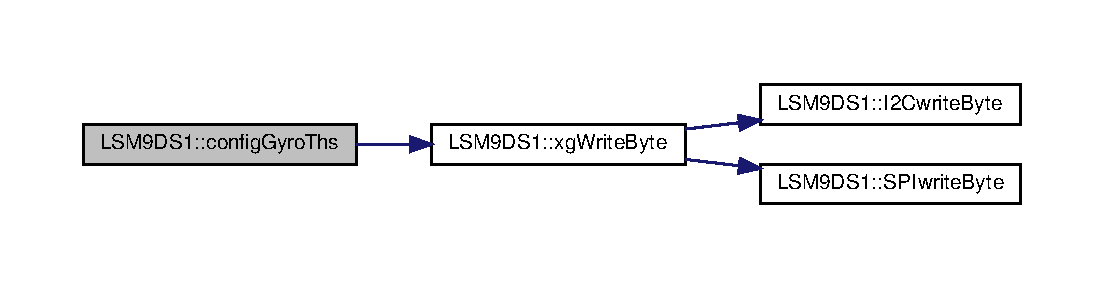
\includegraphics[width=350pt]{classLSM9DS1_ad865cc972960ed476fabd54f698adf6e_cgraph}
\end{center}
\end{figure}
\mbox{\Hypertarget{classLSM9DS1_a1e318c5e7c1d500c3ab2602c46265354}\label{classLSM9DS1_a1e318c5e7c1d500c3ab2602c46265354}} 
\index{L\+S\+M9\+D\+S1@{L\+S\+M9\+D\+S1}!config\+Inactivity@{config\+Inactivity}}
\index{config\+Inactivity@{config\+Inactivity}!L\+S\+M9\+D\+S1@{L\+S\+M9\+D\+S1}}
\subsubsection{\texorpdfstring{config\+Inactivity()}{configInactivity()}}
{\footnotesize\ttfamily void L\+S\+M9\+D\+S1\+::config\+Inactivity (\begin{DoxyParamCaption}\item[{uint8\+\_\+t}]{duration,  }\item[{uint8\+\_\+t}]{threshold,  }\item[{bool}]{sleep\+On }\end{DoxyParamCaption})}



Configures inactivity interrupt parameters. 


\begin{DoxyParams}{Parameters}
{\em duration} & is the inactivity duration. The actual value depends on gyro O\+DR. \\
\hline
{\em threshold} & is the activity threshold. \\
\hline
{\em sleep\+On} & is the gyroscope operating mode during inactivity. true\+: gyroscope in sleep mode false\+: gyroscope in power-\/down \\
\hline
\end{DoxyParams}
Here is the call graph for this function\+:\nopagebreak
\begin{figure}[H]
\begin{center}
\leavevmode
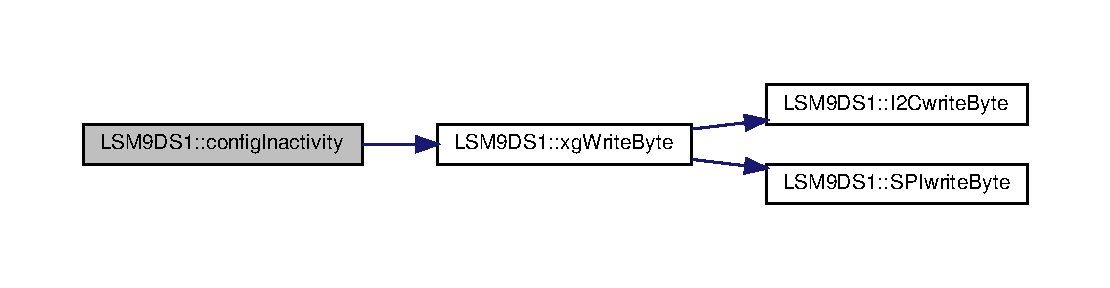
\includegraphics[width=350pt]{classLSM9DS1_a1e318c5e7c1d500c3ab2602c46265354_cgraph}
\end{center}
\end{figure}
\mbox{\Hypertarget{classLSM9DS1_a5b6948b9d4caf57cfe9e0559a0c7f54c}\label{classLSM9DS1_a5b6948b9d4caf57cfe9e0559a0c7f54c}} 
\index{L\+S\+M9\+D\+S1@{L\+S\+M9\+D\+S1}!config\+Int@{config\+Int}}
\index{config\+Int@{config\+Int}!L\+S\+M9\+D\+S1@{L\+S\+M9\+D\+S1}}
\subsubsection{\texorpdfstring{config\+Int()}{configInt()}}
{\footnotesize\ttfamily void L\+S\+M9\+D\+S1\+::config\+Int (\begin{DoxyParamCaption}\item[{interrupt\+\_\+select}]{interupt,  }\item[{uint8\+\_\+t}]{generator,  }\item[{h\+\_\+lactive}]{active\+Low = {\ttfamily INT\+\_\+ACTIVE\+\_\+LOW},  }\item[{pp\+\_\+od}]{push\+Pull = {\ttfamily INT\+\_\+PUSH\+\_\+PULL} }\end{DoxyParamCaption})}



Configures I\+N\+T1 or I\+N\+T2 (Gyro and Accel Interrupts only). 


\begin{DoxyParams}{Parameters}
{\em interrupt} & Select I\+N\+T1 or I\+N\+T2. Possible values\+: X\+G\+\_\+\+I\+N\+T1 or X\+G\+\_\+\+I\+N\+T2 \\
\hline
{\em generator} & Or\textquotesingle{}d combination of interrupt generators. ossible values\+: I\+N\+T\+\_\+\+D\+R\+D\+Y\+\_\+\+XL, I\+N\+T\+\_\+\+D\+R\+D\+Y\+\_\+G, I\+N\+T1\+\_\+\+B\+O\+OT (I\+N\+T1 only), I\+N\+T2\+\_\+\+D\+R\+D\+Y\+\_\+\+T\+E\+MP (I\+N\+T2 only) I\+N\+T\+\_\+\+F\+TH, I\+N\+T\+\_\+\+O\+VR, I\+N\+T\+\_\+\+F\+S\+S5, I\+N\+T\+\_\+\+I\+G\+\_\+\+XL (I\+N\+T1 only), I\+N\+T1\+\_\+\+I\+G\+\_\+G (I\+N\+T1 only), I\+N\+T2\+\_\+\+I\+N\+A\+CT (I\+N\+T2 only). \\
\hline
{\em active\+Low} & interrupts active configuration. Can be either I\+N\+T\+\_\+\+A\+C\+T\+I\+V\+E\+\_\+\+H\+I\+GH or I\+N\+T\+\_\+\+A\+C\+T\+I\+V\+E\+\_\+\+L\+OW. \\
\hline
{\em push\+Pull} & push-\/pulls or open drains interrupt configuration. Can be either I\+N\+T\+\_\+\+P\+U\+S\+H\+\_\+\+P\+U\+LL or I\+N\+T\+\_\+\+O\+P\+E\+N\+\_\+\+D\+R\+A\+IN. \\
\hline
\end{DoxyParams}
Here is the call graph for this function\+:\nopagebreak
\begin{figure}[H]
\begin{center}
\leavevmode
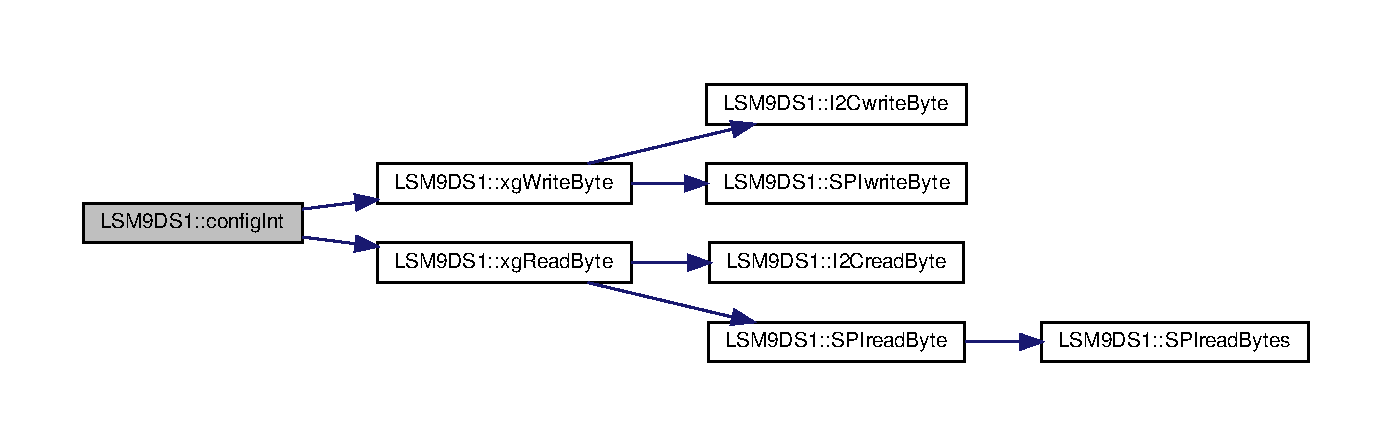
\includegraphics[width=350pt]{classLSM9DS1_a5b6948b9d4caf57cfe9e0559a0c7f54c_cgraph}
\end{center}
\end{figure}
\mbox{\Hypertarget{classLSM9DS1_a54a521668eb63d504d227c6d460723e0}\label{classLSM9DS1_a54a521668eb63d504d227c6d460723e0}} 
\index{L\+S\+M9\+D\+S1@{L\+S\+M9\+D\+S1}!config\+Mag\+Int@{config\+Mag\+Int}}
\index{config\+Mag\+Int@{config\+Mag\+Int}!L\+S\+M9\+D\+S1@{L\+S\+M9\+D\+S1}}
\subsubsection{\texorpdfstring{config\+Mag\+Int()}{configMagInt()}}
{\footnotesize\ttfamily void L\+S\+M9\+D\+S1\+::config\+Mag\+Int (\begin{DoxyParamCaption}\item[{uint8\+\_\+t}]{generator,  }\item[{h\+\_\+lactive}]{active\+Low,  }\item[{bool}]{latch = {\ttfamily true} }\end{DoxyParamCaption})}



Configures Magnetometer Interrupt Generator. 


\begin{DoxyParams}{Parameters}
{\em generator} & interrups axis/high-\/low events. \\
\hline
{\em active\+Low} & interrupts active configuration. Can be either I\+N\+T\+\_\+\+A\+C\+T\+I\+V\+E\+\_\+\+H\+I\+GH or I\+N\+T\+\_\+\+A\+C\+T\+I\+V\+E\+\_\+\+L\+OW. \\
\hline
{\em latch} & latches gyroscope interrupt request. \\
\hline
\end{DoxyParams}
Here is the call graph for this function\+:\nopagebreak
\begin{figure}[H]
\begin{center}
\leavevmode
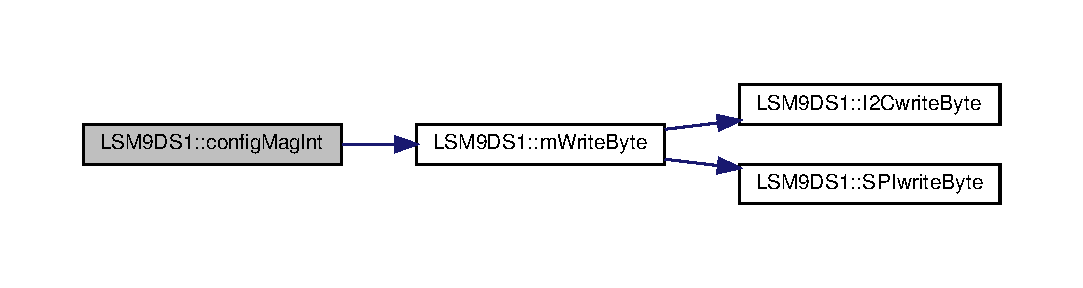
\includegraphics[width=350pt]{classLSM9DS1_a54a521668eb63d504d227c6d460723e0_cgraph}
\end{center}
\end{figure}
\mbox{\Hypertarget{classLSM9DS1_a87cf3dd3a4d9ca79106eb7c1c866a224}\label{classLSM9DS1_a87cf3dd3a4d9ca79106eb7c1c866a224}} 
\index{L\+S\+M9\+D\+S1@{L\+S\+M9\+D\+S1}!config\+Mag\+Ths@{config\+Mag\+Ths}}
\index{config\+Mag\+Ths@{config\+Mag\+Ths}!L\+S\+M9\+D\+S1@{L\+S\+M9\+D\+S1}}
\subsubsection{\texorpdfstring{config\+Mag\+Ths()}{configMagThs()}}
{\footnotesize\ttfamily void L\+S\+M9\+D\+S1\+::config\+Mag\+Ths (\begin{DoxyParamCaption}\item[{uint16\+\_\+t}]{threshold }\end{DoxyParamCaption})}



Configures the threshold of a gyroscope axis. 


\begin{DoxyParams}{Parameters}
{\em threshold} & interrupts threshold. Possible values\+: 0-\/0x7\+FF. Value is equivalent to raw magnetometer value. \\
\hline
\end{DoxyParams}
Here is the call graph for this function\+:\nopagebreak
\begin{figure}[H]
\begin{center}
\leavevmode
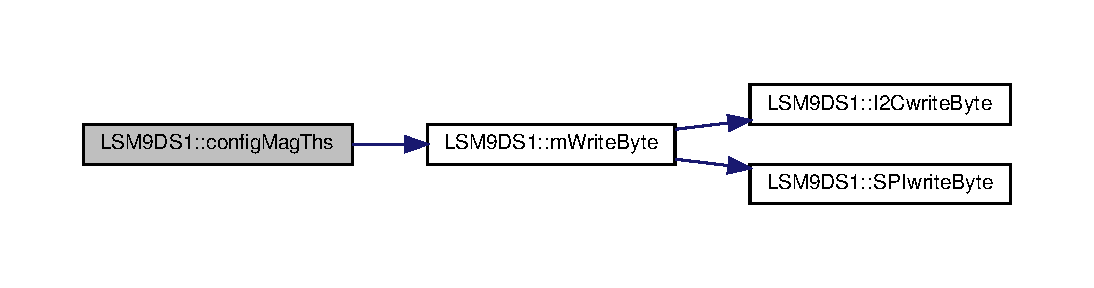
\includegraphics[width=350pt]{classLSM9DS1_a87cf3dd3a4d9ca79106eb7c1c866a224_cgraph}
\end{center}
\end{figure}
\mbox{\Hypertarget{classLSM9DS1_a5f01141131318697838f15d7e5d10f2c}\label{classLSM9DS1_a5f01141131318697838f15d7e5d10f2c}} 
\index{L\+S\+M9\+D\+S1@{L\+S\+M9\+D\+S1}!enable\+F\+I\+FO@{enable\+F\+I\+FO}}
\index{enable\+F\+I\+FO@{enable\+F\+I\+FO}!L\+S\+M9\+D\+S1@{L\+S\+M9\+D\+S1}}
\subsubsection{\texorpdfstring{enable\+F\+I\+F\+O()}{enableFIFO()}}
{\footnotesize\ttfamily void L\+S\+M9\+D\+S1\+::enable\+F\+I\+FO (\begin{DoxyParamCaption}\item[{bool}]{enable = {\ttfamily true} }\end{DoxyParamCaption})}



Enables or disables the F\+I\+FO. 


\begin{DoxyParams}{Parameters}
{\em enable} & F\+I\+FO or diable. True = enable, false = disable. \\
\hline
\end{DoxyParams}
Here is the call graph for this function\+:\nopagebreak
\begin{figure}[H]
\begin{center}
\leavevmode
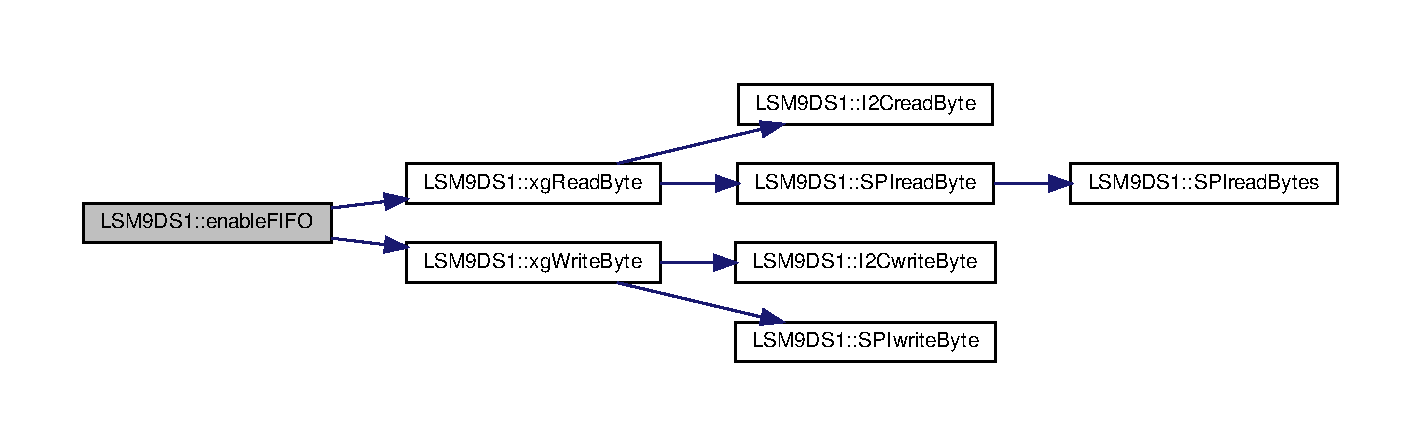
\includegraphics[width=350pt]{classLSM9DS1_a5f01141131318697838f15d7e5d10f2c_cgraph}
\end{center}
\end{figure}
Here is the caller graph for this function\+:\nopagebreak
\begin{figure}[H]
\begin{center}
\leavevmode
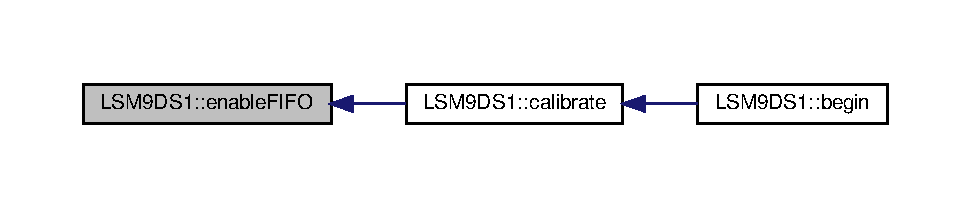
\includegraphics[width=350pt]{classLSM9DS1_a5f01141131318697838f15d7e5d10f2c_icgraph}
\end{center}
\end{figure}
\mbox{\Hypertarget{classLSM9DS1_ae42ae3b368370f977d090ba0e53c7f5c}\label{classLSM9DS1_ae42ae3b368370f977d090ba0e53c7f5c}} 
\index{L\+S\+M9\+D\+S1@{L\+S\+M9\+D\+S1}!get\+Accel\+Int\+Src@{get\+Accel\+Int\+Src}}
\index{get\+Accel\+Int\+Src@{get\+Accel\+Int\+Src}!L\+S\+M9\+D\+S1@{L\+S\+M9\+D\+S1}}
\subsubsection{\texorpdfstring{get\+Accel\+Int\+Src()}{getAccelIntSrc()}}
{\footnotesize\ttfamily uint8\+\_\+t L\+S\+M9\+D\+S1\+::get\+Accel\+Int\+Src (\begin{DoxyParamCaption}{ }\end{DoxyParamCaption})}



Gets contents of accelerometer interrupt source register. 

\begin{DoxyReturn}{Returns}
the contents of accelerometer interrupt source register. 
\end{DoxyReturn}
Here is the call graph for this function\+:\nopagebreak
\begin{figure}[H]
\begin{center}
\leavevmode
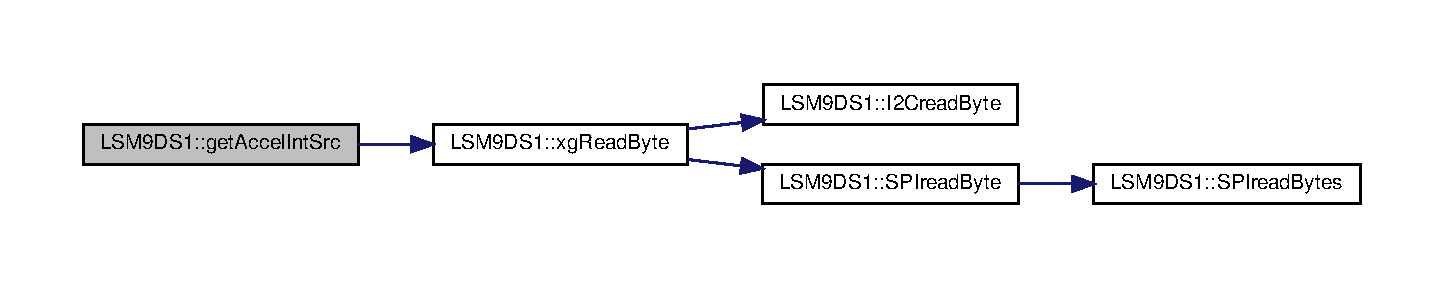
\includegraphics[width=350pt]{classLSM9DS1_ae42ae3b368370f977d090ba0e53c7f5c_cgraph}
\end{center}
\end{figure}
\mbox{\Hypertarget{classLSM9DS1_ac03ef2ff928a25c4a80af7707cd92dc8}\label{classLSM9DS1_ac03ef2ff928a25c4a80af7707cd92dc8}} 
\index{L\+S\+M9\+D\+S1@{L\+S\+M9\+D\+S1}!get\+F\+I\+F\+O\+Samples@{get\+F\+I\+F\+O\+Samples}}
\index{get\+F\+I\+F\+O\+Samples@{get\+F\+I\+F\+O\+Samples}!L\+S\+M9\+D\+S1@{L\+S\+M9\+D\+S1}}
\subsubsection{\texorpdfstring{get\+F\+I\+F\+O\+Samples()}{getFIFOSamples()}}
{\footnotesize\ttfamily uint8\+\_\+t L\+S\+M9\+D\+S1\+::get\+F\+I\+F\+O\+Samples (\begin{DoxyParamCaption}{ }\end{DoxyParamCaption})}



Gets number of F\+I\+FO samples. 

\begin{DoxyReturn}{Returns}
number of F\+I\+FO samples. 
\end{DoxyReturn}
Here is the call graph for this function\+:\nopagebreak
\begin{figure}[H]
\begin{center}
\leavevmode
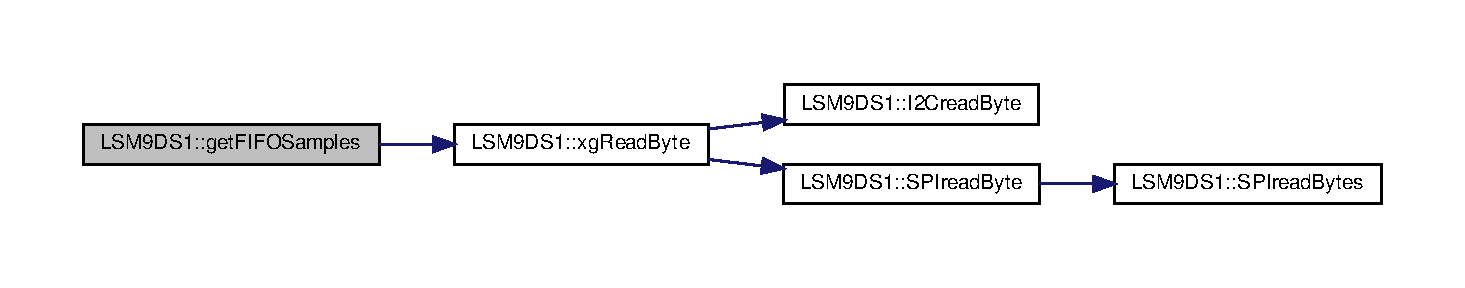
\includegraphics[width=350pt]{classLSM9DS1_ac03ef2ff928a25c4a80af7707cd92dc8_cgraph}
\end{center}
\end{figure}
\mbox{\Hypertarget{classLSM9DS1_aaba6696754df62a411a6a190100f9ca3}\label{classLSM9DS1_aaba6696754df62a411a6a190100f9ca3}} 
\index{L\+S\+M9\+D\+S1@{L\+S\+M9\+D\+S1}!get\+Gyro\+Int\+Src@{get\+Gyro\+Int\+Src}}
\index{get\+Gyro\+Int\+Src@{get\+Gyro\+Int\+Src}!L\+S\+M9\+D\+S1@{L\+S\+M9\+D\+S1}}
\subsubsection{\texorpdfstring{get\+Gyro\+Int\+Src()}{getGyroIntSrc()}}
{\footnotesize\ttfamily uint8\+\_\+t L\+S\+M9\+D\+S1\+::get\+Gyro\+Int\+Src (\begin{DoxyParamCaption}{ }\end{DoxyParamCaption})}



Gets contents of gyroscope interrupt source register. 

\begin{DoxyReturn}{Returns}
the contents of gyroscope interrupt source register. 
\end{DoxyReturn}
Here is the call graph for this function\+:\nopagebreak
\begin{figure}[H]
\begin{center}
\leavevmode
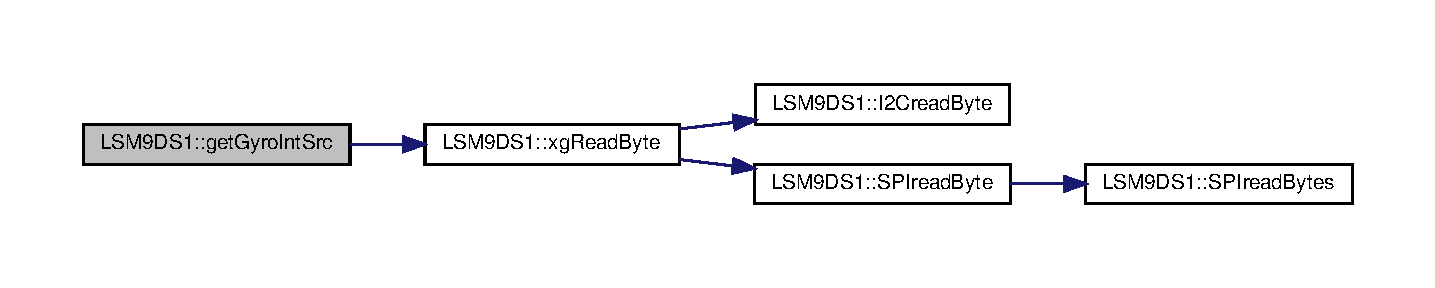
\includegraphics[width=350pt]{classLSM9DS1_aaba6696754df62a411a6a190100f9ca3_cgraph}
\end{center}
\end{figure}
\mbox{\Hypertarget{classLSM9DS1_a9dab029d1d24e49709258d893042d28f}\label{classLSM9DS1_a9dab029d1d24e49709258d893042d28f}} 
\index{L\+S\+M9\+D\+S1@{L\+S\+M9\+D\+S1}!get\+Inactivity@{get\+Inactivity}}
\index{get\+Inactivity@{get\+Inactivity}!L\+S\+M9\+D\+S1@{L\+S\+M9\+D\+S1}}
\subsubsection{\texorpdfstring{get\+Inactivity()}{getInactivity()}}
{\footnotesize\ttfamily uint8\+\_\+t L\+S\+M9\+D\+S1\+::get\+Inactivity (\begin{DoxyParamCaption}{ }\end{DoxyParamCaption})}



Gets status of inactivity interrupt. 

\begin{DoxyReturn}{Returns}
the status of inactivity interrupt. 
\end{DoxyReturn}
Here is the call graph for this function\+:\nopagebreak
\begin{figure}[H]
\begin{center}
\leavevmode
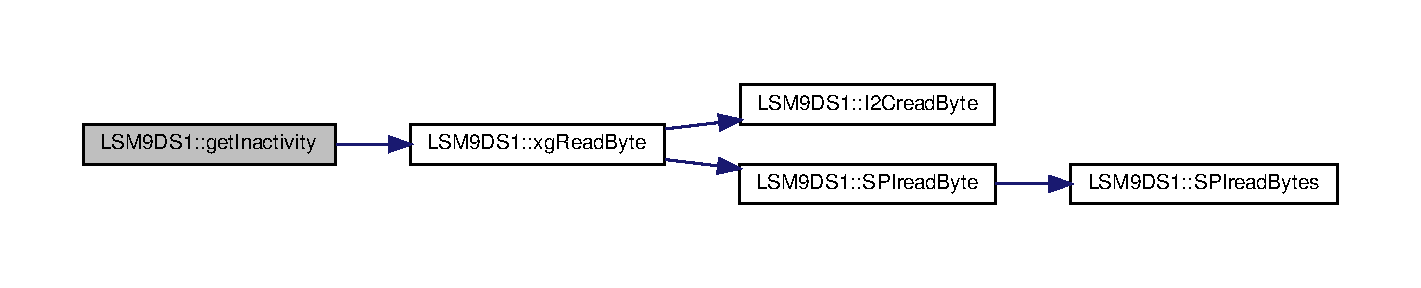
\includegraphics[width=350pt]{classLSM9DS1_a9dab029d1d24e49709258d893042d28f_cgraph}
\end{center}
\end{figure}
\mbox{\Hypertarget{classLSM9DS1_a2bc92a37db982059b89e0a06e7d05a95}\label{classLSM9DS1_a2bc92a37db982059b89e0a06e7d05a95}} 
\index{L\+S\+M9\+D\+S1@{L\+S\+M9\+D\+S1}!get\+Mag\+Int\+Src@{get\+Mag\+Int\+Src}}
\index{get\+Mag\+Int\+Src@{get\+Mag\+Int\+Src}!L\+S\+M9\+D\+S1@{L\+S\+M9\+D\+S1}}
\subsubsection{\texorpdfstring{get\+Mag\+Int\+Src()}{getMagIntSrc()}}
{\footnotesize\ttfamily uint8\+\_\+t L\+S\+M9\+D\+S1\+::get\+Mag\+Int\+Src (\begin{DoxyParamCaption}{ }\end{DoxyParamCaption})}



Gets contents of magnetometer interrupt source register. 

\begin{DoxyReturn}{Returns}
the contents of magnetometer interrupt source register. 
\end{DoxyReturn}
Here is the call graph for this function\+:\nopagebreak
\begin{figure}[H]
\begin{center}
\leavevmode
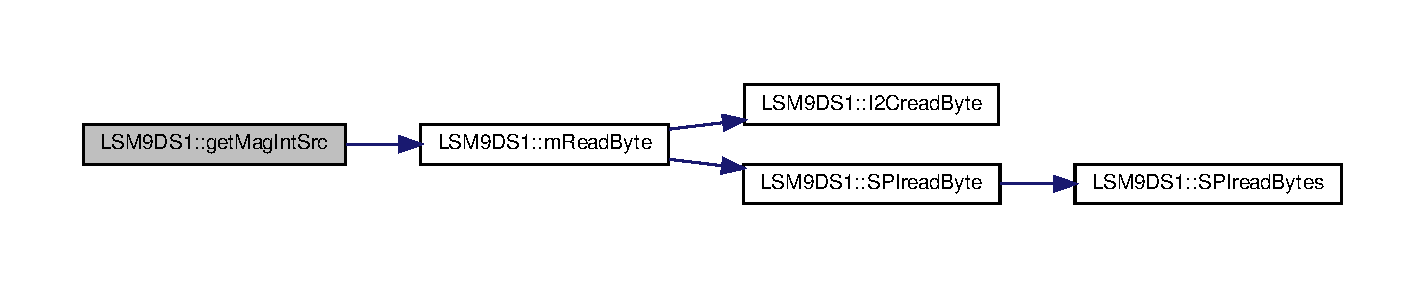
\includegraphics[width=350pt]{classLSM9DS1_a2bc92a37db982059b89e0a06e7d05a95_cgraph}
\end{center}
\end{figure}
\mbox{\Hypertarget{classLSM9DS1_a65b71a03a30f4e8ed1ffd46de3db0560}\label{classLSM9DS1_a65b71a03a30f4e8ed1ffd46de3db0560}} 
\index{L\+S\+M9\+D\+S1@{L\+S\+M9\+D\+S1}!gyro\+Available@{gyro\+Available}}
\index{gyro\+Available@{gyro\+Available}!L\+S\+M9\+D\+S1@{L\+S\+M9\+D\+S1}}
\subsubsection{\texorpdfstring{gyro\+Available()}{gyroAvailable()}}
{\footnotesize\ttfamily uint8\+\_\+t L\+S\+M9\+D\+S1\+::gyro\+Available (\begin{DoxyParamCaption}{ }\end{DoxyParamCaption})}



Polls the gyroscope status register to check if new data is available. 

\begin{DoxyReturn}{Returns}
1 if new data is available, 0 if no new data is available. 
\end{DoxyReturn}
Here is the call graph for this function\+:\nopagebreak
\begin{figure}[H]
\begin{center}
\leavevmode
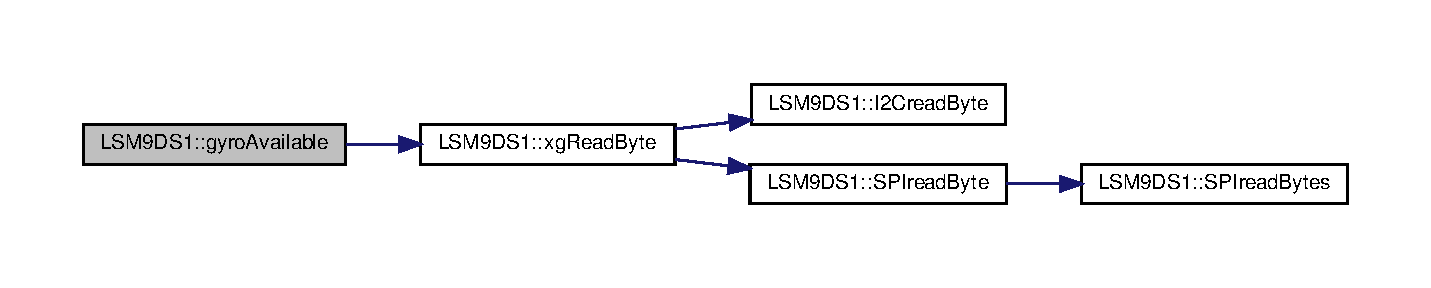
\includegraphics[width=350pt]{classLSM9DS1_a65b71a03a30f4e8ed1ffd46de3db0560_cgraph}
\end{center}
\end{figure}
\mbox{\Hypertarget{classLSM9DS1_a7fc046d4b335494331905fdeb5c81c9e}\label{classLSM9DS1_a7fc046d4b335494331905fdeb5c81c9e}} 
\index{L\+S\+M9\+D\+S1@{L\+S\+M9\+D\+S1}!I2\+Cread\+Byte@{I2\+Cread\+Byte}}
\index{I2\+Cread\+Byte@{I2\+Cread\+Byte}!L\+S\+M9\+D\+S1@{L\+S\+M9\+D\+S1}}
\subsubsection{\texorpdfstring{I2\+Cread\+Byte()}{I2CreadByte()}}
{\footnotesize\ttfamily uint8\+\_\+t L\+S\+M9\+D\+S1\+::\+I2\+Cread\+Byte (\begin{DoxyParamCaption}\item[{uint8\+\_\+t}]{address,  }\item[{uint8\+\_\+t}]{sub\+Address }\end{DoxyParamCaption})\hspace{0.3cm}{\ttfamily [protected]}}



Reads a single byte from a register over I2C. 


\begin{DoxyParams}{Parameters}
{\em address} & the 7-\/bit I2C address of the slave device. \\
\hline
{\em sub\+Address} & the register to be read from. \\
\hline
\end{DoxyParams}
\begin{DoxyReturn}{Returns}
the byte read from the requested address. 
\end{DoxyReturn}
Here is the caller graph for this function\+:\nopagebreak
\begin{figure}[H]
\begin{center}
\leavevmode
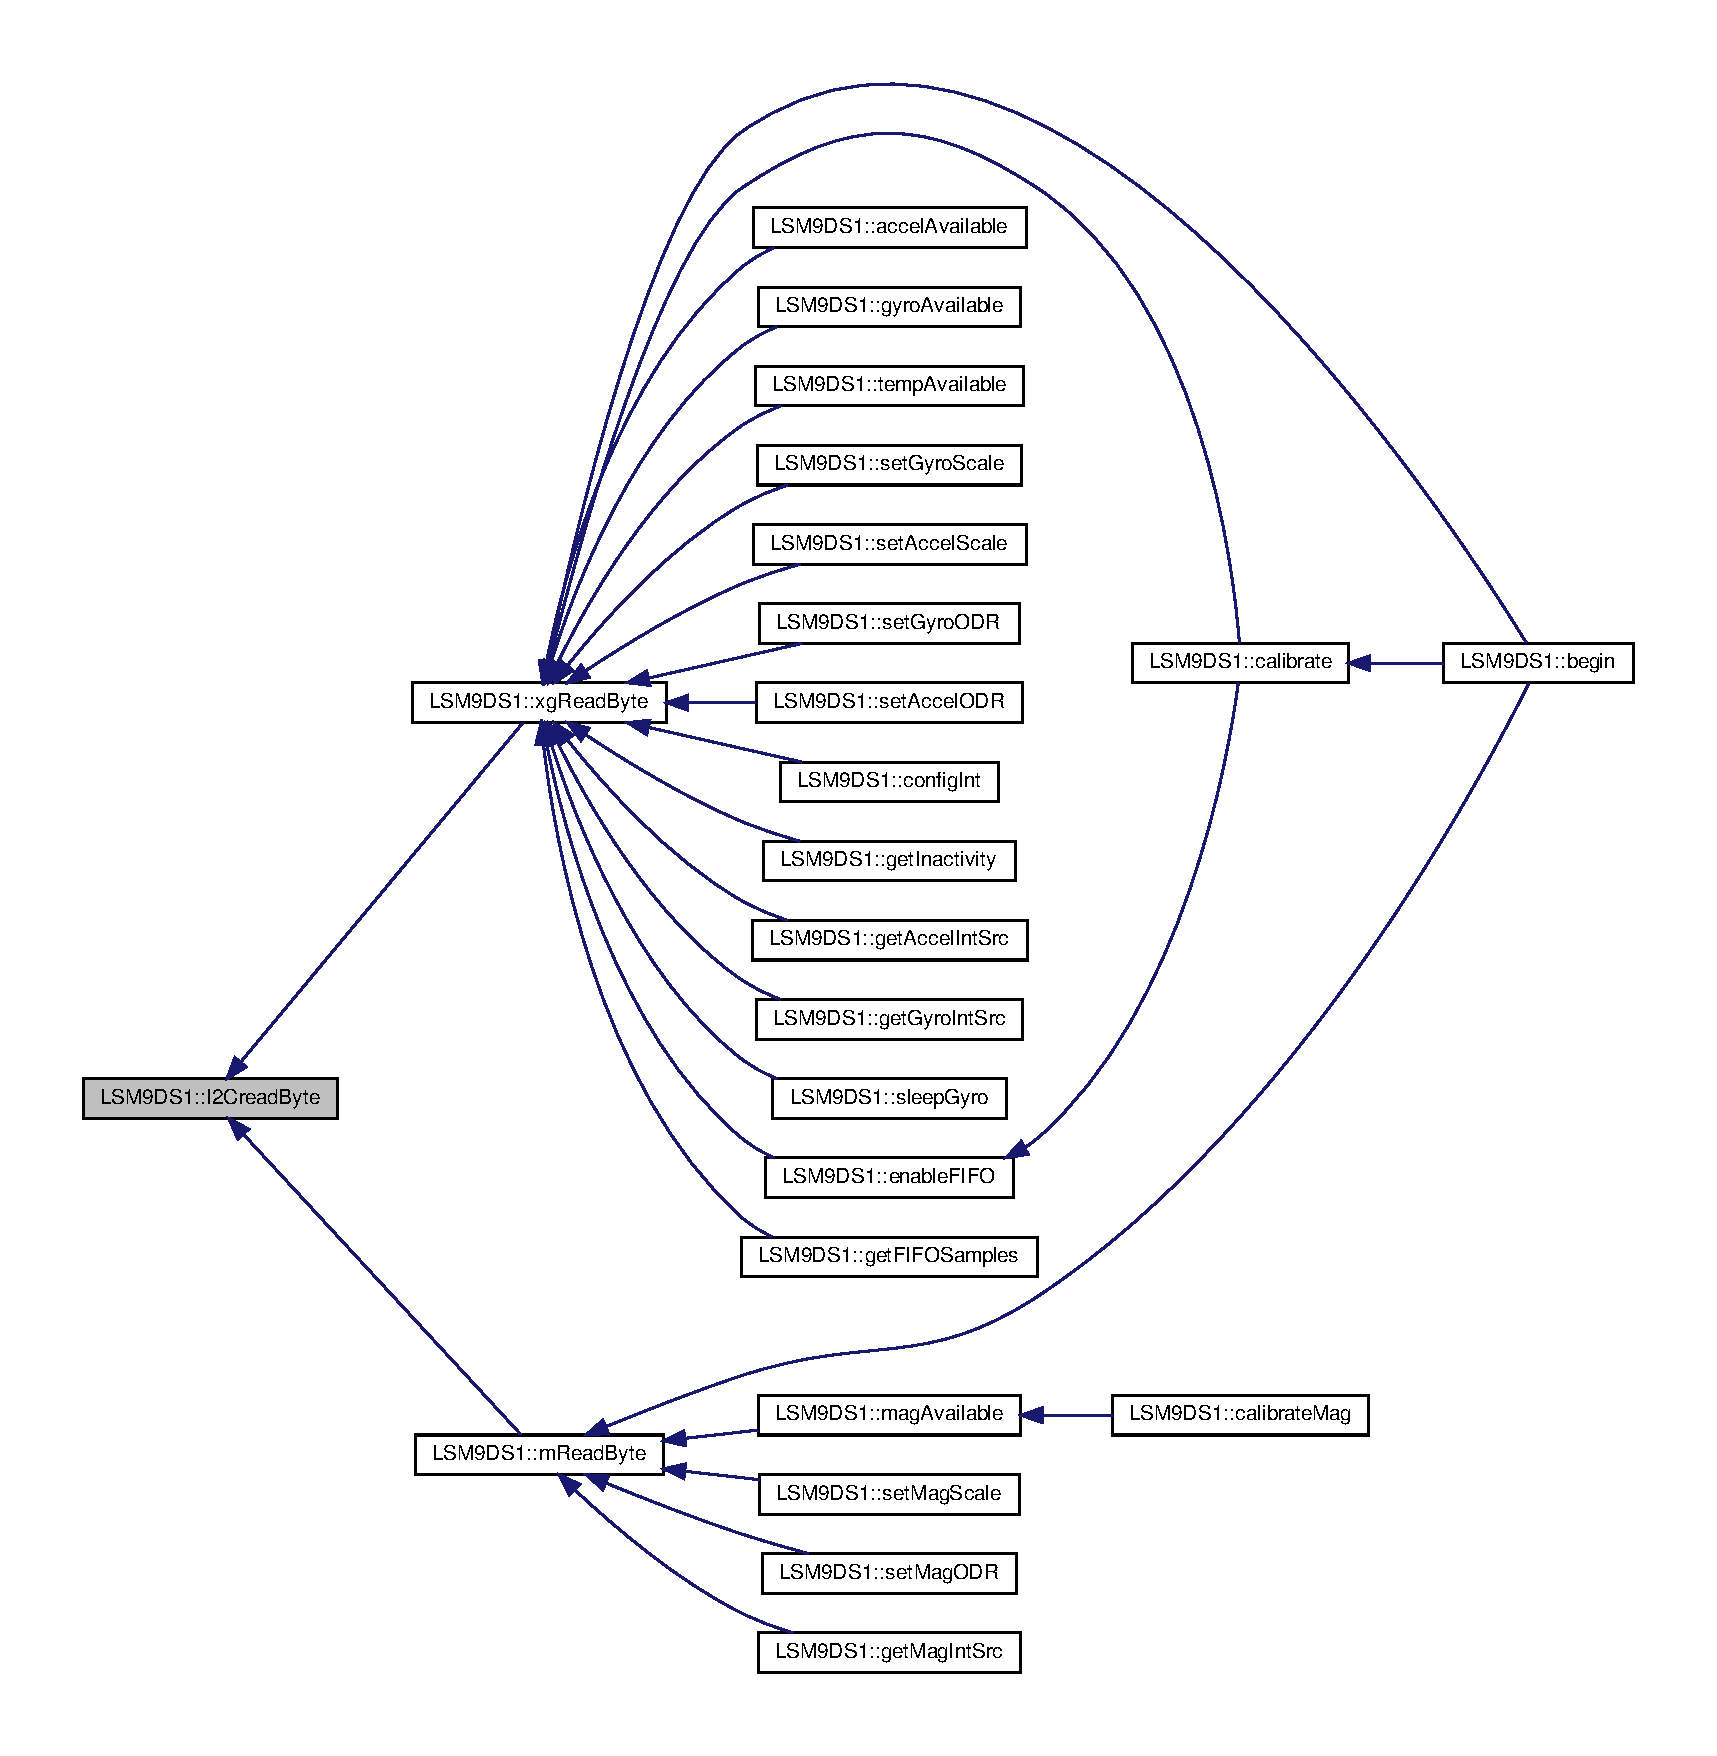
\includegraphics[width=350pt]{classLSM9DS1_a7fc046d4b335494331905fdeb5c81c9e_icgraph}
\end{center}
\end{figure}
\mbox{\Hypertarget{classLSM9DS1_adfc9a22290daddd7787e8023fa8f12cc}\label{classLSM9DS1_adfc9a22290daddd7787e8023fa8f12cc}} 
\index{L\+S\+M9\+D\+S1@{L\+S\+M9\+D\+S1}!I2\+Cread\+Bytes@{I2\+Cread\+Bytes}}
\index{I2\+Cread\+Bytes@{I2\+Cread\+Bytes}!L\+S\+M9\+D\+S1@{L\+S\+M9\+D\+S1}}
\subsubsection{\texorpdfstring{I2\+Cread\+Bytes()}{I2CreadBytes()}}
{\footnotesize\ttfamily uint8\+\_\+t L\+S\+M9\+D\+S1\+::\+I2\+Cread\+Bytes (\begin{DoxyParamCaption}\item[{uint8\+\_\+t}]{address,  }\item[{uint8\+\_\+t}]{sub\+Address,  }\item[{uint8\+\_\+t $\ast$}]{dest,  }\item[{uint8\+\_\+t}]{count }\end{DoxyParamCaption})\hspace{0.3cm}{\ttfamily [protected]}}



Reads a series of bytes, starting at a register via S\+PI. 


\begin{DoxyParams}{Parameters}
{\em address} & the 7-\/bit I2C address of the slave device. \\
\hline
{\em sub\+Address} & the register to begin reading. \\
\hline
{\em dest} & the pointer to an array where we\textquotesingle{}ll store the readings. \\
\hline
{\em count} & number of register to be read. \\
\hline
\end{DoxyParams}
Here is the caller graph for this function\+:\nopagebreak
\begin{figure}[H]
\begin{center}
\leavevmode
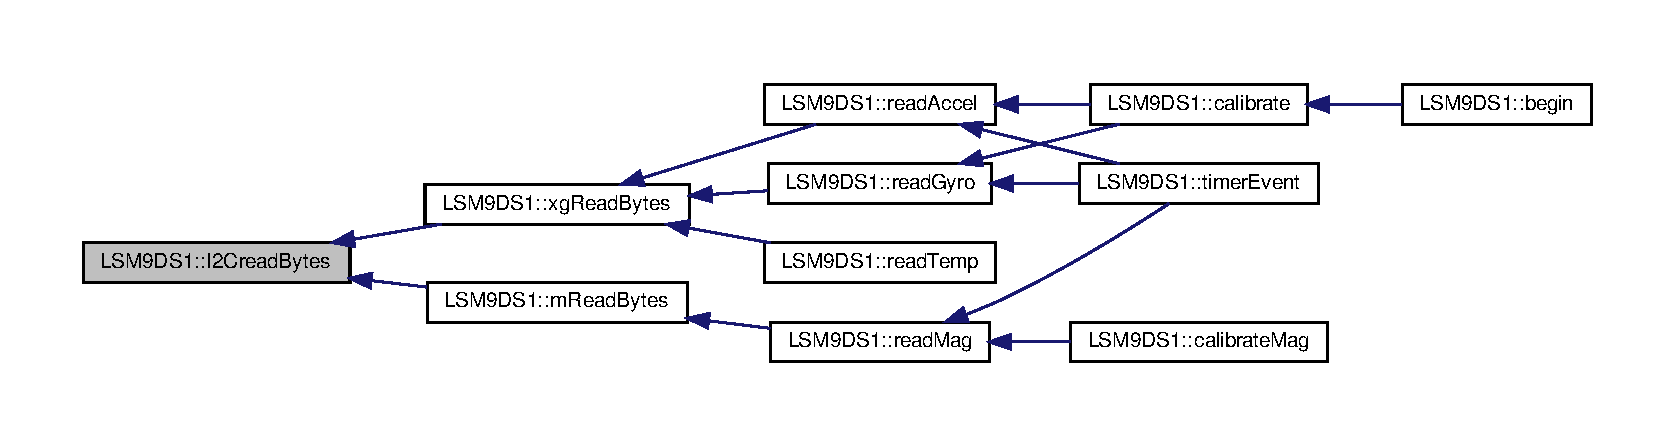
\includegraphics[width=350pt]{classLSM9DS1_adfc9a22290daddd7787e8023fa8f12cc_icgraph}
\end{center}
\end{figure}
\mbox{\Hypertarget{classLSM9DS1_a8e66108a002cc15ec4c0db0a608d20c6}\label{classLSM9DS1_a8e66108a002cc15ec4c0db0a608d20c6}} 
\index{L\+S\+M9\+D\+S1@{L\+S\+M9\+D\+S1}!I2\+Cwrite\+Byte@{I2\+Cwrite\+Byte}}
\index{I2\+Cwrite\+Byte@{I2\+Cwrite\+Byte}!L\+S\+M9\+D\+S1@{L\+S\+M9\+D\+S1}}
\subsubsection{\texorpdfstring{I2\+Cwrite\+Byte()}{I2CwriteByte()}}
{\footnotesize\ttfamily void L\+S\+M9\+D\+S1\+::\+I2\+Cwrite\+Byte (\begin{DoxyParamCaption}\item[{uint8\+\_\+t}]{address,  }\item[{uint8\+\_\+t}]{sub\+Address,  }\item[{uint8\+\_\+t}]{data }\end{DoxyParamCaption})\hspace{0.3cm}{\ttfamily [protected]}}



Writes a byte out of I2C to a register in the device. 


\begin{DoxyParams}{Parameters}
{\em address} & the 7-\/bit I2C address of the slave device. \\
\hline
{\em sub\+Address} & the register to be written to. \\
\hline
{\em data} & byte to be written to the register. \\
\hline
\end{DoxyParams}
Here is the caller graph for this function\+:\nopagebreak
\begin{figure}[H]
\begin{center}
\leavevmode
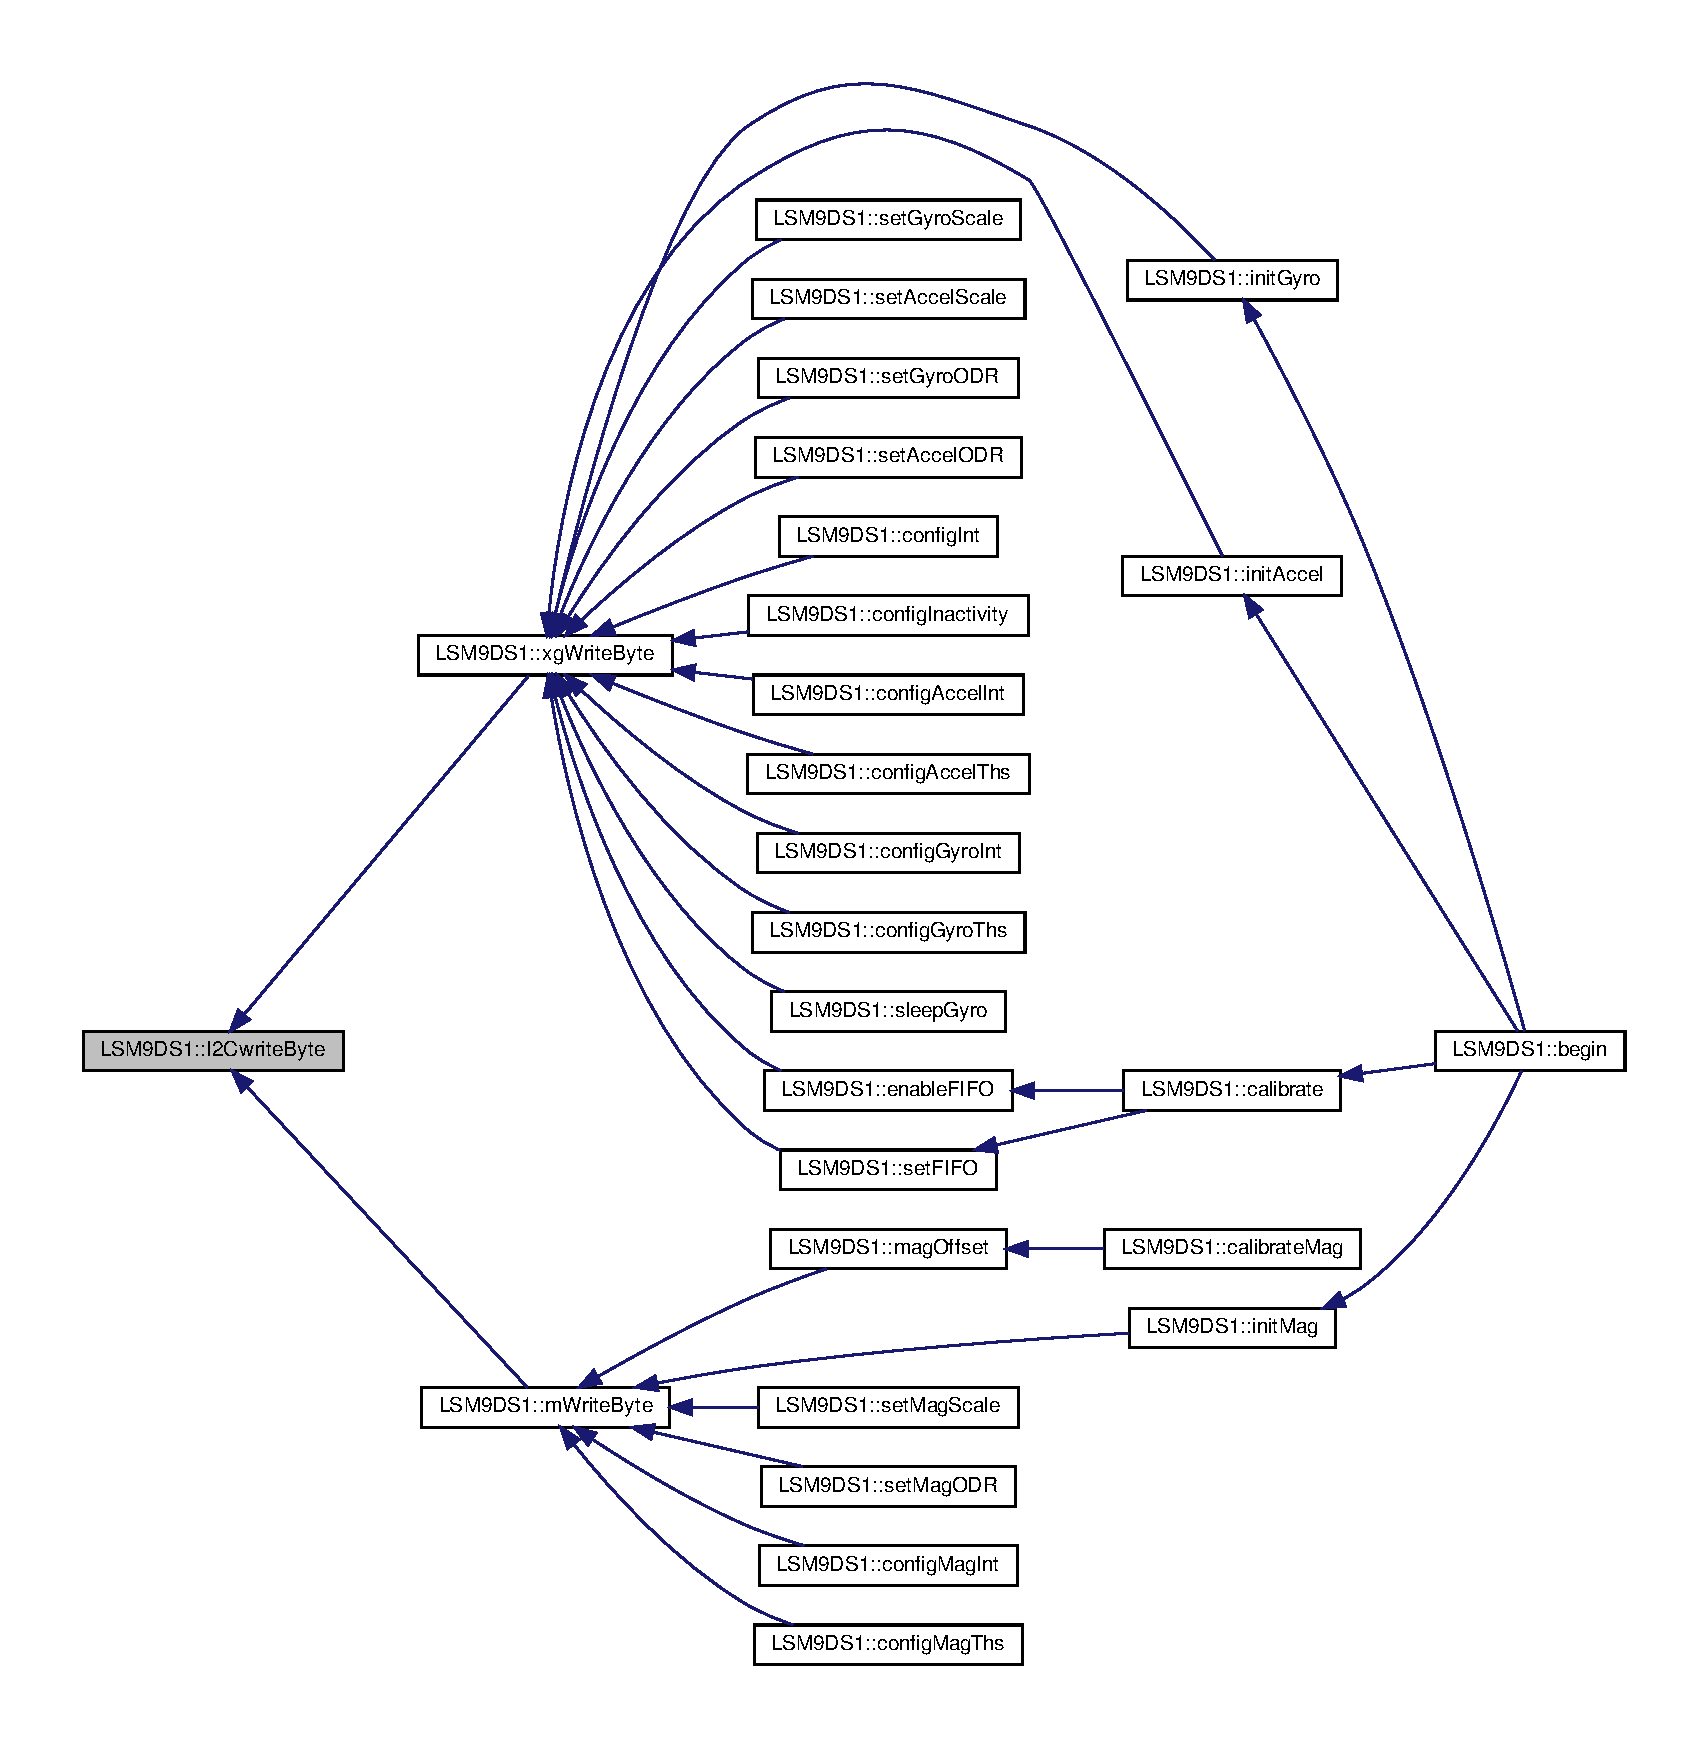
\includegraphics[width=350pt]{classLSM9DS1_a8e66108a002cc15ec4c0db0a608d20c6_icgraph}
\end{center}
\end{figure}
\mbox{\Hypertarget{classLSM9DS1_aa4f74e09e93c0133dc30545d4492849e}\label{classLSM9DS1_aa4f74e09e93c0133dc30545d4492849e}} 
\index{L\+S\+M9\+D\+S1@{L\+S\+M9\+D\+S1}!init@{init}}
\index{init@{init}!L\+S\+M9\+D\+S1@{L\+S\+M9\+D\+S1}}
\subsubsection{\texorpdfstring{init()}{init()}}
{\footnotesize\ttfamily void L\+S\+M9\+D\+S1\+::init (\begin{DoxyParamCaption}\item[{interface\+\_\+mode}]{interface,  }\item[{uint8\+\_\+t}]{xg\+Addr,  }\item[{uint8\+\_\+t}]{m\+Addr }\end{DoxyParamCaption})\hspace{0.3cm}{\ttfamily [protected]}}



Sets up gyro, accel, and mag settings to default. 


\begin{DoxyParams}{Parameters}
{\em interface} & sets the interface mode (I\+M\+U\+\_\+\+M\+O\+D\+E\+\_\+\+I2C or I\+M\+U\+\_\+\+M\+O\+D\+E\+\_\+\+S\+PI). \\
\hline
{\em xg\+Addr} & sets either the I2C address of the accel/gyro or S\+PI chip. Select pin connected to the C\+S\+\_\+\+XG pin. \\
\hline
{\em m\+Addr} & sets either the I2C address of the magnetometer or S\+PI chip select pin connected to the C\+S\+\_\+M pin. \\
\hline
\end{DoxyParams}
Here is the caller graph for this function\+:\nopagebreak
\begin{figure}[H]
\begin{center}
\leavevmode
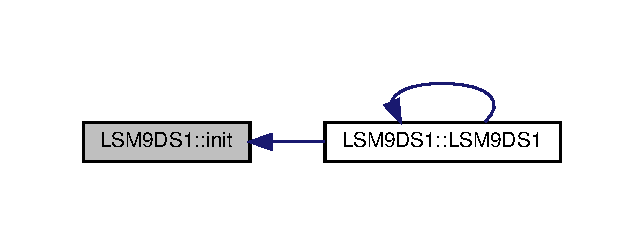
\includegraphics[width=309pt]{classLSM9DS1_aa4f74e09e93c0133dc30545d4492849e_icgraph}
\end{center}
\end{figure}
\mbox{\Hypertarget{classLSM9DS1_a143ff5abf4f7ba8e1c42325859106f84}\label{classLSM9DS1_a143ff5abf4f7ba8e1c42325859106f84}} 
\index{L\+S\+M9\+D\+S1@{L\+S\+M9\+D\+S1}!init\+Accel@{init\+Accel}}
\index{init\+Accel@{init\+Accel}!L\+S\+M9\+D\+S1@{L\+S\+M9\+D\+S1}}
\subsubsection{\texorpdfstring{init\+Accel()}{initAccel()}}
{\footnotesize\ttfamily void L\+S\+M9\+D\+S1\+::init\+Accel (\begin{DoxyParamCaption}{ }\end{DoxyParamCaption})\hspace{0.3cm}{\ttfamily [protected]}}



Sets up the accelerometer to begin reading. 

This function steps through all accelerometer related control registers. Upon exit these registers will be set as\+:
\begin{DoxyItemize}
\item C\+T\+R\+L\+\_\+\+R\+E\+G0\+\_\+\+XM = 0x00\+: F\+I\+FO disabled. H\+PF bypassed. Normal mode.
\item C\+T\+R\+L\+\_\+\+R\+E\+G1\+\_\+\+XM = 0x57\+: 100 Hz data rate. Continuous update. all axes enabled.
\item C\+T\+R\+L\+\_\+\+R\+E\+G2\+\_\+\+XM = 0x00\+: 2g scale. 773 Hz anti-\/alias filter BW.
\item C\+T\+R\+L\+\_\+\+R\+E\+G3\+\_\+\+XM = 0x04\+: Accel data ready signal on I\+N\+T1\+\_\+\+XM pin. 
\end{DoxyItemize}Here is the call graph for this function\+:\nopagebreak
\begin{figure}[H]
\begin{center}
\leavevmode
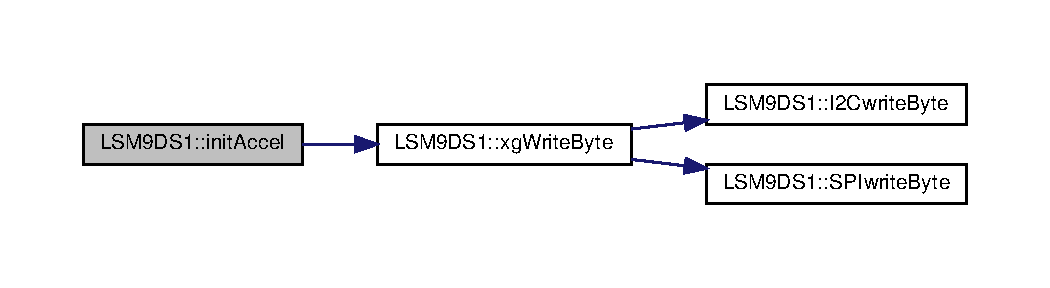
\includegraphics[width=350pt]{classLSM9DS1_a143ff5abf4f7ba8e1c42325859106f84_cgraph}
\end{center}
\end{figure}
Here is the caller graph for this function\+:\nopagebreak
\begin{figure}[H]
\begin{center}
\leavevmode
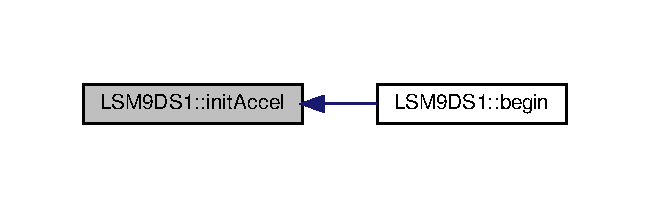
\includegraphics[width=312pt]{classLSM9DS1_a143ff5abf4f7ba8e1c42325859106f84_icgraph}
\end{center}
\end{figure}
\mbox{\Hypertarget{classLSM9DS1_a66a7b02acb28964ffc9362f25988e270}\label{classLSM9DS1_a66a7b02acb28964ffc9362f25988e270}} 
\index{L\+S\+M9\+D\+S1@{L\+S\+M9\+D\+S1}!init\+Gyro@{init\+Gyro}}
\index{init\+Gyro@{init\+Gyro}!L\+S\+M9\+D\+S1@{L\+S\+M9\+D\+S1}}
\subsubsection{\texorpdfstring{init\+Gyro()}{initGyro()}}
{\footnotesize\ttfamily void L\+S\+M9\+D\+S1\+::init\+Gyro (\begin{DoxyParamCaption}{ }\end{DoxyParamCaption})\hspace{0.3cm}{\ttfamily [protected]}}



Sets up the gyroscope to begin reading. 

// \hyperlink{classLSM9DS1_a66a7b02acb28964ffc9362f25988e270}{init\+Gyro()} -- Sets up the gyroscope to begin reading. This function steps through all five gyroscope control registers. Upon exit, the following parameters will be set\+:
\begin{DoxyItemize}
\item C\+T\+R\+L\+\_\+\+R\+E\+G1\+\_\+G = 0x0F\+: Normal operation mode, all axes enabled. 95 Hz O\+DR, 12.\+5 Hz cutoff frequency.
\item C\+T\+R\+L\+\_\+\+R\+E\+G2\+\_\+G = 0x00\+: H\+PF set to normal mode, cutoff frequency set to 7.\+2 Hz (depends on O\+DR).
\item C\+T\+R\+L\+\_\+\+R\+E\+G3\+\_\+G = 0x88\+: Interrupt enabled on I\+N\+T\+\_\+G (set to push-\/pull and active high). Data-\/ready output enabled on D\+R\+D\+Y\+\_\+G.
\item C\+T\+R\+L\+\_\+\+R\+E\+G4\+\_\+G = 0x00\+: Continuous update mode. Data L\+SB stored in lower address. Scale set to 245 D\+PS. S\+PI mode set to 4-\/wire.
\item C\+T\+R\+L\+\_\+\+R\+E\+G5\+\_\+G = 0x00\+: F\+I\+FO disabled. H\+PF disabled. 
\end{DoxyItemize}Here is the call graph for this function\+:\nopagebreak
\begin{figure}[H]
\begin{center}
\leavevmode
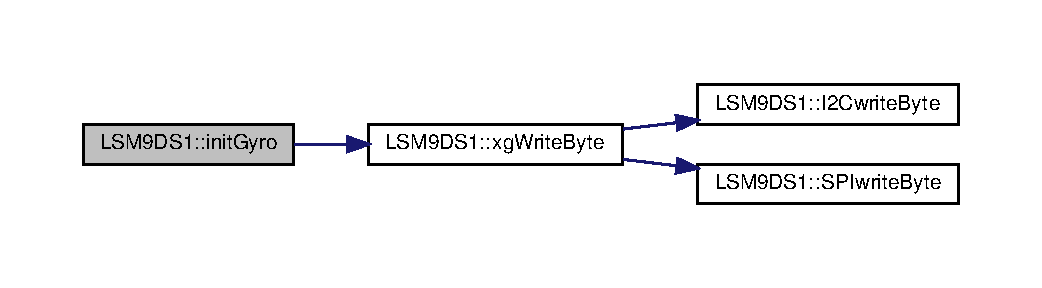
\includegraphics[width=350pt]{classLSM9DS1_a66a7b02acb28964ffc9362f25988e270_cgraph}
\end{center}
\end{figure}
Here is the caller graph for this function\+:\nopagebreak
\begin{figure}[H]
\begin{center}
\leavevmode
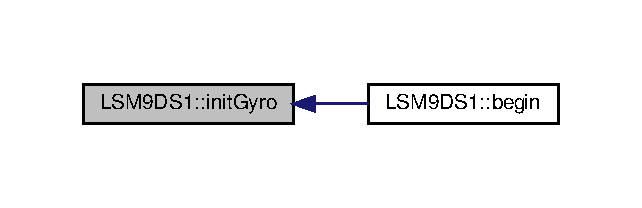
\includegraphics[width=308pt]{classLSM9DS1_a66a7b02acb28964ffc9362f25988e270_icgraph}
\end{center}
\end{figure}
\mbox{\Hypertarget{classLSM9DS1_ae60332c2836bd3f19846b7a44c015ddd}\label{classLSM9DS1_ae60332c2836bd3f19846b7a44c015ddd}} 
\index{L\+S\+M9\+D\+S1@{L\+S\+M9\+D\+S1}!init\+I2C@{init\+I2C}}
\index{init\+I2C@{init\+I2C}!L\+S\+M9\+D\+S1@{L\+S\+M9\+D\+S1}}
\subsubsection{\texorpdfstring{init\+I2\+C()}{initI2C()}}
{\footnotesize\ttfamily void L\+S\+M9\+D\+S1\+::init\+I2C (\begin{DoxyParamCaption}{ }\end{DoxyParamCaption})\hspace{0.3cm}{\ttfamily [protected]}}



Initializes the I2C hardware. 

This function will setup all I2C pins and related hardware. \mbox{\Hypertarget{classLSM9DS1_a492aa6edcf891f273d932636e3cc470d}\label{classLSM9DS1_a492aa6edcf891f273d932636e3cc470d}} 
\index{L\+S\+M9\+D\+S1@{L\+S\+M9\+D\+S1}!init\+Mag@{init\+Mag}}
\index{init\+Mag@{init\+Mag}!L\+S\+M9\+D\+S1@{L\+S\+M9\+D\+S1}}
\subsubsection{\texorpdfstring{init\+Mag()}{initMag()}}
{\footnotesize\ttfamily void L\+S\+M9\+D\+S1\+::init\+Mag (\begin{DoxyParamCaption}{ }\end{DoxyParamCaption})\hspace{0.3cm}{\ttfamily [protected]}}



Sets up the magnetometer to begin reading. 

This function steps through all magnetometer-\/related control registers. Upon exit these registers will be set as\+:
\begin{DoxyItemize}
\item C\+T\+R\+L\+\_\+\+R\+E\+G4\+\_\+\+XM = 0x04\+: Mag data ready signal on I\+N\+T2\+\_\+\+XM pin.
\item C\+T\+R\+L\+\_\+\+R\+E\+G5\+\_\+\+XM = 0x14\+: 100 Hz update rate. Low resolution. Interrupt requests don\textquotesingle{}t latch. Temperature sensor disabled.
\item C\+T\+R\+L\+\_\+\+R\+E\+G6\+\_\+\+XM = 0x00\+: 2 Gs scale.
\item C\+T\+R\+L\+\_\+\+R\+E\+G7\+\_\+\+XM = 0x00\+: Continuous conversion mode. Normal H\+PF mode.
\item I\+N\+T\+\_\+\+C\+T\+R\+L\+\_\+\+R\+E\+G\+\_\+M = 0x09\+: Interrupt active-\/high. Enable interrupts. 
\end{DoxyItemize}Here is the call graph for this function\+:\nopagebreak
\begin{figure}[H]
\begin{center}
\leavevmode
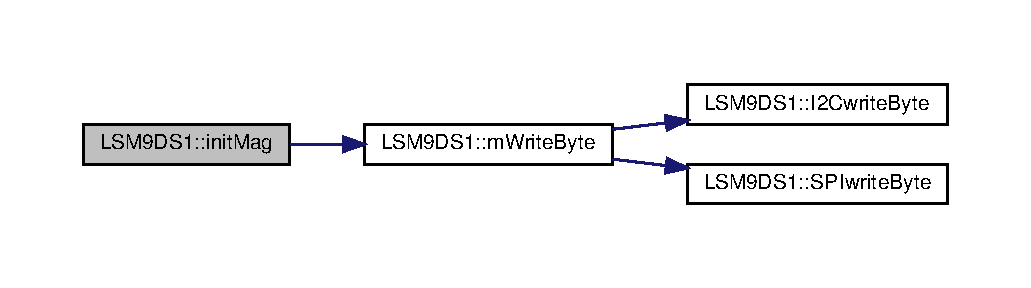
\includegraphics[width=350pt]{classLSM9DS1_a492aa6edcf891f273d932636e3cc470d_cgraph}
\end{center}
\end{figure}
Here is the caller graph for this function\+:\nopagebreak
\begin{figure}[H]
\begin{center}
\leavevmode
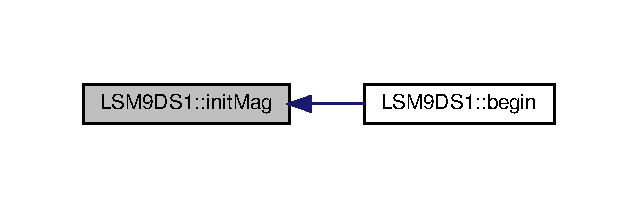
\includegraphics[width=306pt]{classLSM9DS1_a492aa6edcf891f273d932636e3cc470d_icgraph}
\end{center}
\end{figure}
\mbox{\Hypertarget{classLSM9DS1_a4286d5803ab028c657e007ae99acc60a}\label{classLSM9DS1_a4286d5803ab028c657e007ae99acc60a}} 
\index{L\+S\+M9\+D\+S1@{L\+S\+M9\+D\+S1}!init\+S\+PI@{init\+S\+PI}}
\index{init\+S\+PI@{init\+S\+PI}!L\+S\+M9\+D\+S1@{L\+S\+M9\+D\+S1}}
\subsubsection{\texorpdfstring{init\+S\+P\+I()}{initSPI()}}
{\footnotesize\ttfamily void L\+S\+M9\+D\+S1\+::init\+S\+PI (\begin{DoxyParamCaption}{ }\end{DoxyParamCaption})\hspace{0.3cm}{\ttfamily [protected]}}



Initializes the S\+PI hardware. 

This function will setup all S\+PI pins and related hardware. \mbox{\Hypertarget{classLSM9DS1_a85afd29e95bead7b3f0083a9a235d1df}\label{classLSM9DS1_a85afd29e95bead7b3f0083a9a235d1df}} 
\index{L\+S\+M9\+D\+S1@{L\+S\+M9\+D\+S1}!mag\+Available@{mag\+Available}}
\index{mag\+Available@{mag\+Available}!L\+S\+M9\+D\+S1@{L\+S\+M9\+D\+S1}}
\subsubsection{\texorpdfstring{mag\+Available()}{magAvailable()}}
{\footnotesize\ttfamily uint8\+\_\+t L\+S\+M9\+D\+S1\+::mag\+Available (\begin{DoxyParamCaption}\item[{lsm9ds1\+\_\+axis}]{axis = {\ttfamily ALL\+\_\+AXIS} }\end{DoxyParamCaption})}



Polls the temperature status register to check if new data is available. 


\begin{DoxyParams}{Parameters}
{\em axis} & can either be X\+\_\+\+A\+X\+IS, Y\+\_\+\+A\+X\+IS, Z\+\_\+\+A\+X\+IS, to check for new data on one specific axis or A\+L\+L\+\_\+\+A\+X\+IS (default) to check for new data on all axes. \\
\hline
\end{DoxyParams}
\begin{DoxyReturn}{Returns}
1 if new data is available, 0 if no new data is available. 
\end{DoxyReturn}
Here is the call graph for this function\+:\nopagebreak
\begin{figure}[H]
\begin{center}
\leavevmode
\includegraphics[width=350pt]{classLSM9DS1_a85afd29e95bead7b3f0083a9a235d1df_cgraph}
\end{center}
\end{figure}
Here is the caller graph for this function\+:\nopagebreak
\begin{figure}[H]
\begin{center}
\leavevmode
\includegraphics[width=350pt]{classLSM9DS1_a85afd29e95bead7b3f0083a9a235d1df_icgraph}
\end{center}
\end{figure}
\mbox{\Hypertarget{classLSM9DS1_a0d461614bd058b082c94481dc916c18b}\label{classLSM9DS1_a0d461614bd058b082c94481dc916c18b}} 
\index{L\+S\+M9\+D\+S1@{L\+S\+M9\+D\+S1}!mag\+Offset@{mag\+Offset}}
\index{mag\+Offset@{mag\+Offset}!L\+S\+M9\+D\+S1@{L\+S\+M9\+D\+S1}}
\subsubsection{\texorpdfstring{mag\+Offset()}{magOffset()}}
{\footnotesize\ttfamily void L\+S\+M9\+D\+S1\+::mag\+Offset (\begin{DoxyParamCaption}\item[{uint8\+\_\+t}]{axis,  }\item[{int16\+\_\+t}]{offset }\end{DoxyParamCaption})}



Sets the magnetometer offset. 


\begin{DoxyParams}{Parameters}
{\em axis} & the axis for which the offset should be set. \\
\hline
{\em offset} & the offset that should be set. \\
\hline
\end{DoxyParams}
Here is the call graph for this function\+:\nopagebreak
\begin{figure}[H]
\begin{center}
\leavevmode
\includegraphics[width=350pt]{classLSM9DS1_a0d461614bd058b082c94481dc916c18b_cgraph}
\end{center}
\end{figure}
Here is the caller graph for this function\+:\nopagebreak
\begin{figure}[H]
\begin{center}
\leavevmode
\includegraphics[width=350pt]{classLSM9DS1_a0d461614bd058b082c94481dc916c18b_icgraph}
\end{center}
\end{figure}
\mbox{\Hypertarget{classLSM9DS1_ae4e470321567e4f93fc09f4cc6cd9efa}\label{classLSM9DS1_ae4e470321567e4f93fc09f4cc6cd9efa}} 
\index{L\+S\+M9\+D\+S1@{L\+S\+M9\+D\+S1}!m\+Read\+Byte@{m\+Read\+Byte}}
\index{m\+Read\+Byte@{m\+Read\+Byte}!L\+S\+M9\+D\+S1@{L\+S\+M9\+D\+S1}}
\subsubsection{\texorpdfstring{m\+Read\+Byte()}{mReadByte()}}
{\footnotesize\ttfamily uint8\+\_\+t L\+S\+M9\+D\+S1\+::m\+Read\+Byte (\begin{DoxyParamCaption}\item[{uint8\+\_\+t}]{sub\+Address }\end{DoxyParamCaption})\hspace{0.3cm}{\ttfamily [protected]}}



Reads a byte from a specified gyroscope register. 


\begin{DoxyParams}{Parameters}
{\em sub\+Address} & the register to be read from. \\
\hline
\end{DoxyParams}
\begin{DoxyReturn}{Returns}
a 8-\/bit value read from the requested address. 
\end{DoxyReturn}
Here is the call graph for this function\+:\nopagebreak
\begin{figure}[H]
\begin{center}
\leavevmode
\includegraphics[width=350pt]{classLSM9DS1_ae4e470321567e4f93fc09f4cc6cd9efa_cgraph}
\end{center}
\end{figure}
Here is the caller graph for this function\+:\nopagebreak
\begin{figure}[H]
\begin{center}
\leavevmode
\includegraphics[width=350pt]{classLSM9DS1_ae4e470321567e4f93fc09f4cc6cd9efa_icgraph}
\end{center}
\end{figure}
\mbox{\Hypertarget{classLSM9DS1_acfdf9862cad1e66c9fb61a17bfbe7477}\label{classLSM9DS1_acfdf9862cad1e66c9fb61a17bfbe7477}} 
\index{L\+S\+M9\+D\+S1@{L\+S\+M9\+D\+S1}!m\+Read\+Bytes@{m\+Read\+Bytes}}
\index{m\+Read\+Bytes@{m\+Read\+Bytes}!L\+S\+M9\+D\+S1@{L\+S\+M9\+D\+S1}}
\subsubsection{\texorpdfstring{m\+Read\+Bytes()}{mReadBytes()}}
{\footnotesize\ttfamily void L\+S\+M9\+D\+S1\+::m\+Read\+Bytes (\begin{DoxyParamCaption}\item[{uint8\+\_\+t}]{sub\+Address,  }\item[{uint8\+\_\+t $\ast$}]{dest,  }\item[{uint8\+\_\+t}]{count }\end{DoxyParamCaption})\hspace{0.3cm}{\ttfamily [protected]}}



Reads a number of bytes -- beginning at an address and incrementing from there -- from the gyroscope. 


\begin{DoxyParams}{Parameters}
{\em sub\+Address} & the register to be read from. \\
\hline
{\em dest} & a pointer to an array of uint8\+\_\+t\textquotesingle{}s. Values read will be stored in here on return. \\
\hline
{\em count} & the number of bytes to be read. \\
\hline
\end{DoxyParams}
Here is the call graph for this function\+:\nopagebreak
\begin{figure}[H]
\begin{center}
\leavevmode
\includegraphics[width=350pt]{classLSM9DS1_acfdf9862cad1e66c9fb61a17bfbe7477_cgraph}
\end{center}
\end{figure}
Here is the caller graph for this function\+:\nopagebreak
\begin{figure}[H]
\begin{center}
\leavevmode
\includegraphics[width=350pt]{classLSM9DS1_acfdf9862cad1e66c9fb61a17bfbe7477_icgraph}
\end{center}
\end{figure}
\mbox{\Hypertarget{classLSM9DS1_afc171c924102c97fa1d88fa7f48bd167}\label{classLSM9DS1_afc171c924102c97fa1d88fa7f48bd167}} 
\index{L\+S\+M9\+D\+S1@{L\+S\+M9\+D\+S1}!m\+Write\+Byte@{m\+Write\+Byte}}
\index{m\+Write\+Byte@{m\+Write\+Byte}!L\+S\+M9\+D\+S1@{L\+S\+M9\+D\+S1}}
\subsubsection{\texorpdfstring{m\+Write\+Byte()}{mWriteByte()}}
{\footnotesize\ttfamily void L\+S\+M9\+D\+S1\+::m\+Write\+Byte (\begin{DoxyParamCaption}\item[{uint8\+\_\+t}]{sub\+Address,  }\item[{uint8\+\_\+t}]{data }\end{DoxyParamCaption})\hspace{0.3cm}{\ttfamily [protected]}}



Writes a byte to a register in the gyroscope. 


\begin{DoxyParams}{Parameters}
{\em sub\+Address} & the register to be written to. \\
\hline
{\em data} & the data to be written into the register. \\
\hline
\end{DoxyParams}
Here is the call graph for this function\+:\nopagebreak
\begin{figure}[H]
\begin{center}
\leavevmode
\includegraphics[width=350pt]{classLSM9DS1_afc171c924102c97fa1d88fa7f48bd167_cgraph}
\end{center}
\end{figure}
Here is the caller graph for this function\+:\nopagebreak
\begin{figure}[H]
\begin{center}
\leavevmode
\includegraphics[width=350pt]{classLSM9DS1_afc171c924102c97fa1d88fa7f48bd167_icgraph}
\end{center}
\end{figure}
\mbox{\Hypertarget{classLSM9DS1_a9953684a1ff652a7d3a4d91e72bccaa1}\label{classLSM9DS1_a9953684a1ff652a7d3a4d91e72bccaa1}} 
\index{L\+S\+M9\+D\+S1@{L\+S\+M9\+D\+S1}!read\+Accel@{read\+Accel}}
\index{read\+Accel@{read\+Accel}!L\+S\+M9\+D\+S1@{L\+S\+M9\+D\+S1}}
\subsubsection{\texorpdfstring{read\+Accel()}{readAccel()}\hspace{0.1cm}{\footnotesize\ttfamily [1/2]}}
{\footnotesize\ttfamily void L\+S\+M9\+D\+S1\+::read\+Accel (\begin{DoxyParamCaption}{ }\end{DoxyParamCaption})}



Reads the accelerometer output registers. 

This function will read all six accelerometer output registers. The readings are stored in the class\textquotesingle{} ax, ay, and az variables. Read those {\itshape after} calling \hyperlink{classLSM9DS1_a9953684a1ff652a7d3a4d91e72bccaa1}{read\+Accel()}. Here is the call graph for this function\+:\nopagebreak
\begin{figure}[H]
\begin{center}
\leavevmode
\includegraphics[width=350pt]{classLSM9DS1_a9953684a1ff652a7d3a4d91e72bccaa1_cgraph}
\end{center}
\end{figure}
Here is the caller graph for this function\+:\nopagebreak
\begin{figure}[H]
\begin{center}
\leavevmode
\includegraphics[width=350pt]{classLSM9DS1_a9953684a1ff652a7d3a4d91e72bccaa1_icgraph}
\end{center}
\end{figure}
\mbox{\Hypertarget{classLSM9DS1_acbe3bfc0b8db7fe3f77893d22c394594}\label{classLSM9DS1_acbe3bfc0b8db7fe3f77893d22c394594}} 
\index{L\+S\+M9\+D\+S1@{L\+S\+M9\+D\+S1}!read\+Accel@{read\+Accel}}
\index{read\+Accel@{read\+Accel}!L\+S\+M9\+D\+S1@{L\+S\+M9\+D\+S1}}
\subsubsection{\texorpdfstring{read\+Accel()}{readAccel()}\hspace{0.1cm}{\footnotesize\ttfamily [2/2]}}
{\footnotesize\ttfamily int16\+\_\+t L\+S\+M9\+D\+S1\+::read\+Accel (\begin{DoxyParamCaption}\item[{lsm9ds1\+\_\+axis}]{axis }\end{DoxyParamCaption})}



Reads a specific axis of the accelerometer. 

\mbox{[}axis\mbox{]} can be any of X\+\_\+\+A\+X\+IS, Y\+\_\+\+A\+X\+IS, or Z\+\_\+\+A\+X\+IS.


\begin{DoxyParams}{Parameters}
{\em axis} & can either be can be either X\+\_\+\+A\+X\+IS, Y\+\_\+\+A\+X\+IS, or Z\+\_\+\+A\+X\+IS. \\
\hline
\end{DoxyParams}
\begin{DoxyReturn}{Returns}
a 16-\/bit signed integer with sensor data on requested axis. 
\end{DoxyReturn}
Here is the call graph for this function\+:\nopagebreak
\begin{figure}[H]
\begin{center}
\leavevmode
\includegraphics[width=350pt]{classLSM9DS1_acbe3bfc0b8db7fe3f77893d22c394594_cgraph}
\end{center}
\end{figure}
\mbox{\Hypertarget{classLSM9DS1_a56e9710cb538a4c7f7ab94c2ca256ce9}\label{classLSM9DS1_a56e9710cb538a4c7f7ab94c2ca256ce9}} 
\index{L\+S\+M9\+D\+S1@{L\+S\+M9\+D\+S1}!read\+Gyro@{read\+Gyro}}
\index{read\+Gyro@{read\+Gyro}!L\+S\+M9\+D\+S1@{L\+S\+M9\+D\+S1}}
\subsubsection{\texorpdfstring{read\+Gyro()}{readGyro()}\hspace{0.1cm}{\footnotesize\ttfamily [1/2]}}
{\footnotesize\ttfamily void L\+S\+M9\+D\+S1\+::read\+Gyro (\begin{DoxyParamCaption}{ }\end{DoxyParamCaption})}



Reads the gyroscope output registers. 

This function will read all six gyroscope output registers. The readings are stored in the class\textquotesingle{} gx, gy, and gz variables. Read those {\itshape after} calling \hyperlink{classLSM9DS1_a56e9710cb538a4c7f7ab94c2ca256ce9}{read\+Gyro()}. Here is the call graph for this function\+:\nopagebreak
\begin{figure}[H]
\begin{center}
\leavevmode
\includegraphics[width=350pt]{classLSM9DS1_a56e9710cb538a4c7f7ab94c2ca256ce9_cgraph}
\end{center}
\end{figure}
Here is the caller graph for this function\+:\nopagebreak
\begin{figure}[H]
\begin{center}
\leavevmode
\includegraphics[width=350pt]{classLSM9DS1_a56e9710cb538a4c7f7ab94c2ca256ce9_icgraph}
\end{center}
\end{figure}
\mbox{\Hypertarget{classLSM9DS1_adc1b37609a6c850328b16da4f911cefd}\label{classLSM9DS1_adc1b37609a6c850328b16da4f911cefd}} 
\index{L\+S\+M9\+D\+S1@{L\+S\+M9\+D\+S1}!read\+Gyro@{read\+Gyro}}
\index{read\+Gyro@{read\+Gyro}!L\+S\+M9\+D\+S1@{L\+S\+M9\+D\+S1}}
\subsubsection{\texorpdfstring{read\+Gyro()}{readGyro()}\hspace{0.1cm}{\footnotesize\ttfamily [2/2]}}
{\footnotesize\ttfamily int16\+\_\+t L\+S\+M9\+D\+S1\+::read\+Gyro (\begin{DoxyParamCaption}\item[{lsm9ds1\+\_\+axis}]{axis }\end{DoxyParamCaption})}



Reads a specific axis of the gyroscope. 

\mbox{[}axis\mbox{]} can be any of X\+\_\+\+A\+X\+IS, Y\+\_\+\+A\+X\+IS, or Z\+\_\+\+A\+X\+IS.


\begin{DoxyParams}{Parameters}
{\em axis} & can either be can be either X\+\_\+\+A\+X\+IS, Y\+\_\+\+A\+X\+IS, or Z\+\_\+\+A\+X\+IS. \\
\hline
\end{DoxyParams}
\begin{DoxyReturn}{Returns}
a 16-\/bit signed integer with sensor data on requested axis. 
\end{DoxyReturn}
Here is the call graph for this function\+:\nopagebreak
\begin{figure}[H]
\begin{center}
\leavevmode
\includegraphics[width=350pt]{classLSM9DS1_adc1b37609a6c850328b16da4f911cefd_cgraph}
\end{center}
\end{figure}
\mbox{\Hypertarget{classLSM9DS1_ae127cf75aa5f3c5421e49363795dcd38}\label{classLSM9DS1_ae127cf75aa5f3c5421e49363795dcd38}} 
\index{L\+S\+M9\+D\+S1@{L\+S\+M9\+D\+S1}!read\+Mag@{read\+Mag}}
\index{read\+Mag@{read\+Mag}!L\+S\+M9\+D\+S1@{L\+S\+M9\+D\+S1}}
\subsubsection{\texorpdfstring{read\+Mag()}{readMag()}\hspace{0.1cm}{\footnotesize\ttfamily [1/2]}}
{\footnotesize\ttfamily void L\+S\+M9\+D\+S1\+::read\+Mag (\begin{DoxyParamCaption}{ }\end{DoxyParamCaption})}



Reads the magnetometer output registers. 

This function will read all six magnetometer output registers. The readings are stored in the class\textquotesingle{} ax, ay, and az variables. Read those {\itshape after} calling \hyperlink{classLSM9DS1_ae127cf75aa5f3c5421e49363795dcd38}{read\+Mag()}. Here is the call graph for this function\+:\nopagebreak
\begin{figure}[H]
\begin{center}
\leavevmode
\includegraphics[width=350pt]{classLSM9DS1_ae127cf75aa5f3c5421e49363795dcd38_cgraph}
\end{center}
\end{figure}
Here is the caller graph for this function\+:\nopagebreak
\begin{figure}[H]
\begin{center}
\leavevmode
\includegraphics[width=344pt]{classLSM9DS1_ae127cf75aa5f3c5421e49363795dcd38_icgraph}
\end{center}
\end{figure}
\mbox{\Hypertarget{classLSM9DS1_a615fd3ab32a9af833ef9899663100330}\label{classLSM9DS1_a615fd3ab32a9af833ef9899663100330}} 
\index{L\+S\+M9\+D\+S1@{L\+S\+M9\+D\+S1}!read\+Mag@{read\+Mag}}
\index{read\+Mag@{read\+Mag}!L\+S\+M9\+D\+S1@{L\+S\+M9\+D\+S1}}
\subsubsection{\texorpdfstring{read\+Mag()}{readMag()}\hspace{0.1cm}{\footnotesize\ttfamily [2/2]}}
{\footnotesize\ttfamily int16\+\_\+t L\+S\+M9\+D\+S1\+::read\+Mag (\begin{DoxyParamCaption}\item[{lsm9ds1\+\_\+axis}]{axis }\end{DoxyParamCaption})}



Reads a specific axis of the magnetometer. 

\mbox{[}axis\mbox{]} can be any of X\+\_\+\+A\+X\+IS, Y\+\_\+\+A\+X\+IS, or Z\+\_\+\+A\+X\+IS.


\begin{DoxyParams}{Parameters}
{\em axis} & can either be can be either X\+\_\+\+A\+X\+IS, Y\+\_\+\+A\+X\+IS, or Z\+\_\+\+A\+X\+IS. \\
\hline
\end{DoxyParams}
\begin{DoxyReturn}{Returns}
a 16-\/bit signed integer with sensor data on requested axis. 
\end{DoxyReturn}
Here is the call graph for this function\+:\nopagebreak
\begin{figure}[H]
\begin{center}
\leavevmode
\includegraphics[width=350pt]{classLSM9DS1_a615fd3ab32a9af833ef9899663100330_cgraph}
\end{center}
\end{figure}
\mbox{\Hypertarget{classLSM9DS1_aca21a51dc79a1287b97ed9c326e2080b}\label{classLSM9DS1_aca21a51dc79a1287b97ed9c326e2080b}} 
\index{L\+S\+M9\+D\+S1@{L\+S\+M9\+D\+S1}!read\+Temp@{read\+Temp}}
\index{read\+Temp@{read\+Temp}!L\+S\+M9\+D\+S1@{L\+S\+M9\+D\+S1}}
\subsubsection{\texorpdfstring{read\+Temp()}{readTemp()}}
{\footnotesize\ttfamily void L\+S\+M9\+D\+S1\+::read\+Temp (\begin{DoxyParamCaption}{ }\end{DoxyParamCaption})}



Reads the temperature output registers. 

This function will read two temperature output registers. The readings are stored in the class\textquotesingle{} temperature variables. Read those {\itshape after} calling \hyperlink{classLSM9DS1_aca21a51dc79a1287b97ed9c326e2080b}{read\+Temp()}. Here is the call graph for this function\+:\nopagebreak
\begin{figure}[H]
\begin{center}
\leavevmode
\includegraphics[width=350pt]{classLSM9DS1_aca21a51dc79a1287b97ed9c326e2080b_cgraph}
\end{center}
\end{figure}
\mbox{\Hypertarget{classLSM9DS1_a76d72839cdecc3f1c4ee6fff578182c5}\label{classLSM9DS1_a76d72839cdecc3f1c4ee6fff578182c5}} 
\index{L\+S\+M9\+D\+S1@{L\+S\+M9\+D\+S1}!set\+Accel\+O\+DR@{set\+Accel\+O\+DR}}
\index{set\+Accel\+O\+DR@{set\+Accel\+O\+DR}!L\+S\+M9\+D\+S1@{L\+S\+M9\+D\+S1}}
\subsubsection{\texorpdfstring{set\+Accel\+O\+D\+R()}{setAccelODR()}}
{\footnotesize\ttfamily void L\+S\+M9\+D\+S1\+::set\+Accel\+O\+DR (\begin{DoxyParamCaption}\item[{uint8\+\_\+t}]{a\+Rate }\end{DoxyParamCaption})}



Sets the output data rate and bandwidth of the accelerometer. 


\begin{DoxyParams}{Parameters}
{\em a\+Rate} & is the desired output rate and cutoff frequency of the accel. \\
\hline
\end{DoxyParams}
Here is the call graph for this function\+:\nopagebreak
\begin{figure}[H]
\begin{center}
\leavevmode
\includegraphics[width=350pt]{classLSM9DS1_a76d72839cdecc3f1c4ee6fff578182c5_cgraph}
\end{center}
\end{figure}
\mbox{\Hypertarget{classLSM9DS1_a8656d2de1ff9cc4cb76214e4561d02c4}\label{classLSM9DS1_a8656d2de1ff9cc4cb76214e4561d02c4}} 
\index{L\+S\+M9\+D\+S1@{L\+S\+M9\+D\+S1}!set\+Accel\+Scale@{set\+Accel\+Scale}}
\index{set\+Accel\+Scale@{set\+Accel\+Scale}!L\+S\+M9\+D\+S1@{L\+S\+M9\+D\+S1}}
\subsubsection{\texorpdfstring{set\+Accel\+Scale()}{setAccelScale()}}
{\footnotesize\ttfamily void L\+S\+M9\+D\+S1\+::set\+Accel\+Scale (\begin{DoxyParamCaption}\item[{uint8\+\_\+t}]{a\+Scl }\end{DoxyParamCaption})}



Sets the full-\/scale range of the accelerometer. 

This function can be called to set the scale of the accelerometer to 2, 4, 6, 8, or 16 g\textquotesingle{}s.


\begin{DoxyParams}{Parameters}
{\em a\+Scl} & is the desired accelerometer scale. Must be one of five possible values from the accel\+\_\+scale. \\
\hline
\end{DoxyParams}
Here is the call graph for this function\+:\nopagebreak
\begin{figure}[H]
\begin{center}
\leavevmode
\includegraphics[width=350pt]{classLSM9DS1_a8656d2de1ff9cc4cb76214e4561d02c4_cgraph}
\end{center}
\end{figure}
\mbox{\Hypertarget{classLSM9DS1_a3102ea02c253af39e3b43ee55b94d716}\label{classLSM9DS1_a3102ea02c253af39e3b43ee55b94d716}} 
\index{L\+S\+M9\+D\+S1@{L\+S\+M9\+D\+S1}!set\+Callback@{set\+Callback}}
\index{set\+Callback@{set\+Callback}!L\+S\+M9\+D\+S1@{L\+S\+M9\+D\+S1}}
\subsubsection{\texorpdfstring{set\+Callback()}{setCallback()}}
{\footnotesize\ttfamily void L\+S\+M9\+D\+S1\+::set\+Callback (\begin{DoxyParamCaption}\item[{\hyperlink{classLSM9DS1callback}{L\+S\+M9\+D\+S1callback} $\ast$}]{cb }\end{DoxyParamCaption})\hspace{0.3cm}{\ttfamily [inline]}}



Sets a callback. 


\begin{DoxyParams}{Parameters}
{\em cb} & the callback to be set. \\
\hline
\end{DoxyParams}
\mbox{\Hypertarget{classLSM9DS1_a0ec4a93a34545af1acc336bae9b360f1}\label{classLSM9DS1_a0ec4a93a34545af1acc336bae9b360f1}} 
\index{L\+S\+M9\+D\+S1@{L\+S\+M9\+D\+S1}!set\+F\+I\+FO@{set\+F\+I\+FO}}
\index{set\+F\+I\+FO@{set\+F\+I\+FO}!L\+S\+M9\+D\+S1@{L\+S\+M9\+D\+S1}}
\subsubsection{\texorpdfstring{set\+F\+I\+F\+O()}{setFIFO()}}
{\footnotesize\ttfamily void L\+S\+M9\+D\+S1\+::set\+F\+I\+FO (\begin{DoxyParamCaption}\item[{fifo\+Mode\+\_\+type}]{fifo\+Mode,  }\item[{uint8\+\_\+t}]{fifo\+Ths }\end{DoxyParamCaption})}



Configures F\+I\+FO mode and Threshold. 


\begin{DoxyParams}{Parameters}
{\em fifo\+Mode} & sets F\+I\+FO mode to off, F\+I\+FO (stop when full), continuous, bypass. Possible inputs\+: F\+I\+F\+O\+\_\+\+O\+FF, F\+I\+F\+O\+\_\+\+T\+HS, F\+I\+F\+O\+\_\+\+C\+O\+N\+T\+\_\+\+T\+R\+I\+G\+G\+ER, F\+I\+F\+O\+\_\+\+O\+F\+F\+\_\+\+T\+R\+I\+G\+G\+ER, F\+I\+F\+O\+\_\+\+C\+O\+NT. \\
\hline
{\em fifo\+Ths} & sets F\+I\+FO threshold level. Any value from 0-\/0x1F is acceptable. \\
\hline
\end{DoxyParams}
Here is the call graph for this function\+:\nopagebreak
\begin{figure}[H]
\begin{center}
\leavevmode
\includegraphics[width=350pt]{classLSM9DS1_a0ec4a93a34545af1acc336bae9b360f1_cgraph}
\end{center}
\end{figure}
Here is the caller graph for this function\+:\nopagebreak
\begin{figure}[H]
\begin{center}
\leavevmode
\includegraphics[width=350pt]{classLSM9DS1_a0ec4a93a34545af1acc336bae9b360f1_icgraph}
\end{center}
\end{figure}
\mbox{\Hypertarget{classLSM9DS1_ab8fc33c8da4fc5c379e880ff57d331fa}\label{classLSM9DS1_ab8fc33c8da4fc5c379e880ff57d331fa}} 
\index{L\+S\+M9\+D\+S1@{L\+S\+M9\+D\+S1}!set\+Gyro\+O\+DR@{set\+Gyro\+O\+DR}}
\index{set\+Gyro\+O\+DR@{set\+Gyro\+O\+DR}!L\+S\+M9\+D\+S1@{L\+S\+M9\+D\+S1}}
\subsubsection{\texorpdfstring{set\+Gyro\+O\+D\+R()}{setGyroODR()}}
{\footnotesize\ttfamily void L\+S\+M9\+D\+S1\+::set\+Gyro\+O\+DR (\begin{DoxyParamCaption}\item[{uint8\+\_\+t}]{g\+Rate }\end{DoxyParamCaption})}



Sets the output data rate and bandwidth of the gyroscope. 


\begin{DoxyParams}{Parameters}
{\em g\+Rate} & is the desired output rate and cutoff frequency of the gyro. \\
\hline
\end{DoxyParams}
Here is the call graph for this function\+:\nopagebreak
\begin{figure}[H]
\begin{center}
\leavevmode
\includegraphics[width=350pt]{classLSM9DS1_ab8fc33c8da4fc5c379e880ff57d331fa_cgraph}
\end{center}
\end{figure}
\mbox{\Hypertarget{classLSM9DS1_a115d304ebcdc8c701f3e5a5d397250aa}\label{classLSM9DS1_a115d304ebcdc8c701f3e5a5d397250aa}} 
\index{L\+S\+M9\+D\+S1@{L\+S\+M9\+D\+S1}!set\+Gyro\+Scale@{set\+Gyro\+Scale}}
\index{set\+Gyro\+Scale@{set\+Gyro\+Scale}!L\+S\+M9\+D\+S1@{L\+S\+M9\+D\+S1}}
\subsubsection{\texorpdfstring{set\+Gyro\+Scale()}{setGyroScale()}}
{\footnotesize\ttfamily void L\+S\+M9\+D\+S1\+::set\+Gyro\+Scale (\begin{DoxyParamCaption}\item[{uint16\+\_\+t}]{g\+Scl }\end{DoxyParamCaption})}



Sets the full-\/scale range of the gyroscope. 

This function can be called to set the scale of the gyroscope to 245, 500, or 200 degrees per second.


\begin{DoxyParams}{Parameters}
{\em g\+Scl} & is the desired gyroscope scale. \\
\hline
\end{DoxyParams}
Here is the call graph for this function\+:\nopagebreak
\begin{figure}[H]
\begin{center}
\leavevmode
\includegraphics[width=350pt]{classLSM9DS1_a115d304ebcdc8c701f3e5a5d397250aa_cgraph}
\end{center}
\end{figure}
\mbox{\Hypertarget{classLSM9DS1_a8bc672fba680edc468a643fd58046b41}\label{classLSM9DS1_a8bc672fba680edc468a643fd58046b41}} 
\index{L\+S\+M9\+D\+S1@{L\+S\+M9\+D\+S1}!set\+Mag\+O\+DR@{set\+Mag\+O\+DR}}
\index{set\+Mag\+O\+DR@{set\+Mag\+O\+DR}!L\+S\+M9\+D\+S1@{L\+S\+M9\+D\+S1}}
\subsubsection{\texorpdfstring{set\+Mag\+O\+D\+R()}{setMagODR()}}
{\footnotesize\ttfamily void L\+S\+M9\+D\+S1\+::set\+Mag\+O\+DR (\begin{DoxyParamCaption}\item[{uint8\+\_\+t}]{m\+Rate }\end{DoxyParamCaption})}



Sets the output data rate and bandwidth of the magnetometer. 


\begin{DoxyParams}{Parameters}
{\em m\+Rate} & is the desired output rate and cutoff frequency of the mag. \\
\hline
\end{DoxyParams}
Here is the call graph for this function\+:\nopagebreak
\begin{figure}[H]
\begin{center}
\leavevmode
\includegraphics[width=350pt]{classLSM9DS1_a8bc672fba680edc468a643fd58046b41_cgraph}
\end{center}
\end{figure}
\mbox{\Hypertarget{classLSM9DS1_ad7604159a07b0d088cdfb6ba4a0093b0}\label{classLSM9DS1_ad7604159a07b0d088cdfb6ba4a0093b0}} 
\index{L\+S\+M9\+D\+S1@{L\+S\+M9\+D\+S1}!set\+Mag\+Scale@{set\+Mag\+Scale}}
\index{set\+Mag\+Scale@{set\+Mag\+Scale}!L\+S\+M9\+D\+S1@{L\+S\+M9\+D\+S1}}
\subsubsection{\texorpdfstring{set\+Mag\+Scale()}{setMagScale()}}
{\footnotesize\ttfamily void L\+S\+M9\+D\+S1\+::set\+Mag\+Scale (\begin{DoxyParamCaption}\item[{uint8\+\_\+t}]{m\+Scl }\end{DoxyParamCaption})}



Sets the full-\/scale range of the magnetometer. 

This function can be called to set the scale of the magnetometer to 2, 4, 8, or 12 Gs.


\begin{DoxyParams}{Parameters}
{\em m\+Scl} & is the desired magnetometer scale. Must be one of four possible values from the mag\+\_\+scale. \\
\hline
\end{DoxyParams}
Here is the call graph for this function\+:\nopagebreak
\begin{figure}[H]
\begin{center}
\leavevmode
\includegraphics[width=350pt]{classLSM9DS1_ad7604159a07b0d088cdfb6ba4a0093b0_cgraph}
\end{center}
\end{figure}
\mbox{\Hypertarget{classLSM9DS1_a13b61812069b399547f177b0b0af8fe3}\label{classLSM9DS1_a13b61812069b399547f177b0b0af8fe3}} 
\index{L\+S\+M9\+D\+S1@{L\+S\+M9\+D\+S1}!sleep\+Gyro@{sleep\+Gyro}}
\index{sleep\+Gyro@{sleep\+Gyro}!L\+S\+M9\+D\+S1@{L\+S\+M9\+D\+S1}}
\subsubsection{\texorpdfstring{sleep\+Gyro()}{sleepGyro()}}
{\footnotesize\ttfamily void L\+S\+M9\+D\+S1\+::sleep\+Gyro (\begin{DoxyParamCaption}\item[{bool}]{enable = {\ttfamily true} }\end{DoxyParamCaption})}



Sets gyro to sleep or wake. 


\begin{DoxyParams}{Parameters}
{\em enable} & gyro to sleep or wake. True = sleep, false = wake. \\
\hline
\end{DoxyParams}
Here is the call graph for this function\+:\nopagebreak
\begin{figure}[H]
\begin{center}
\leavevmode
\includegraphics[width=350pt]{classLSM9DS1_a13b61812069b399547f177b0b0af8fe3_cgraph}
\end{center}
\end{figure}
\mbox{\Hypertarget{classLSM9DS1_a6f0f50bb5e9b702d5a19c7441a3f9d8b}\label{classLSM9DS1_a6f0f50bb5e9b702d5a19c7441a3f9d8b}} 
\index{L\+S\+M9\+D\+S1@{L\+S\+M9\+D\+S1}!S\+P\+Iread\+Byte@{S\+P\+Iread\+Byte}}
\index{S\+P\+Iread\+Byte@{S\+P\+Iread\+Byte}!L\+S\+M9\+D\+S1@{L\+S\+M9\+D\+S1}}
\subsubsection{\texorpdfstring{S\+P\+Iread\+Byte()}{SPIreadByte()}}
{\footnotesize\ttfamily uint8\+\_\+t L\+S\+M9\+D\+S1\+::\+S\+P\+Iread\+Byte (\begin{DoxyParamCaption}\item[{uint8\+\_\+t}]{cs\+Pin,  }\item[{uint8\+\_\+t}]{sub\+Address }\end{DoxyParamCaption})\hspace{0.3cm}{\ttfamily [protected]}}



Reads a single byte from a register over S\+PI. 


\begin{DoxyParams}{Parameters}
{\em cs\+Pin} & the chip select pin of the slave device. \\
\hline
{\em sub\+Address} & the register to be read from. \\
\hline
\end{DoxyParams}
\begin{DoxyReturn}{Returns}
the byte read from the requested address. 
\end{DoxyReturn}
Here is the call graph for this function\+:\nopagebreak
\begin{figure}[H]
\begin{center}
\leavevmode
\includegraphics[width=350pt]{classLSM9DS1_a6f0f50bb5e9b702d5a19c7441a3f9d8b_cgraph}
\end{center}
\end{figure}
Here is the caller graph for this function\+:\nopagebreak
\begin{figure}[H]
\begin{center}
\leavevmode
\includegraphics[width=350pt]{classLSM9DS1_a6f0f50bb5e9b702d5a19c7441a3f9d8b_icgraph}
\end{center}
\end{figure}
\mbox{\Hypertarget{classLSM9DS1_a26c0f164454eba84e6486033b7061d11}\label{classLSM9DS1_a26c0f164454eba84e6486033b7061d11}} 
\index{L\+S\+M9\+D\+S1@{L\+S\+M9\+D\+S1}!S\+P\+Iread\+Bytes@{S\+P\+Iread\+Bytes}}
\index{S\+P\+Iread\+Bytes@{S\+P\+Iread\+Bytes}!L\+S\+M9\+D\+S1@{L\+S\+M9\+D\+S1}}
\subsubsection{\texorpdfstring{S\+P\+Iread\+Bytes()}{SPIreadBytes()}}
{\footnotesize\ttfamily void L\+S\+M9\+D\+S1\+::\+S\+P\+Iread\+Bytes (\begin{DoxyParamCaption}\item[{uint8\+\_\+t}]{cs\+Pin,  }\item[{uint8\+\_\+t}]{sub\+Address,  }\item[{uint8\+\_\+t $\ast$}]{dest,  }\item[{uint8\+\_\+t}]{count }\end{DoxyParamCaption})\hspace{0.3cm}{\ttfamily [protected]}}



Initializes the S\+PI hardware. 


\begin{DoxyParams}{Parameters}
{\em } & \\
\hline
\end{DoxyParams}
Here is the caller graph for this function\+:\nopagebreak
\begin{figure}[H]
\begin{center}
\leavevmode
\includegraphics[width=350pt]{classLSM9DS1_a26c0f164454eba84e6486033b7061d11_icgraph}
\end{center}
\end{figure}
\mbox{\Hypertarget{classLSM9DS1_a83321c9d6ec50f6b9944907d2be482cd}\label{classLSM9DS1_a83321c9d6ec50f6b9944907d2be482cd}} 
\index{L\+S\+M9\+D\+S1@{L\+S\+M9\+D\+S1}!S\+P\+Iwrite\+Byte@{S\+P\+Iwrite\+Byte}}
\index{S\+P\+Iwrite\+Byte@{S\+P\+Iwrite\+Byte}!L\+S\+M9\+D\+S1@{L\+S\+M9\+D\+S1}}
\subsubsection{\texorpdfstring{S\+P\+Iwrite\+Byte()}{SPIwriteByte()}}
{\footnotesize\ttfamily void L\+S\+M9\+D\+S1\+::\+S\+P\+Iwrite\+Byte (\begin{DoxyParamCaption}\item[{uint8\+\_\+t}]{cs\+Pin,  }\item[{uint8\+\_\+t}]{sub\+Address,  }\item[{uint8\+\_\+t}]{data }\end{DoxyParamCaption})\hspace{0.3cm}{\ttfamily [protected]}}



Writes a byte out of S\+PI to a register in the device. 


\begin{DoxyParams}{Parameters}
{\em cs\+Pin} & the chip select pin of the slave device. \\
\hline
{\em sub\+Address} & the register to be written to. \\
\hline
{\em data} & byte to be written into the register. \\
\hline
\end{DoxyParams}
Here is the caller graph for this function\+:\nopagebreak
\begin{figure}[H]
\begin{center}
\leavevmode
\includegraphics[width=350pt]{classLSM9DS1_a83321c9d6ec50f6b9944907d2be482cd_icgraph}
\end{center}
\end{figure}
\mbox{\Hypertarget{classLSM9DS1_aaf6683c6f3f0281d5222b74f580f321b}\label{classLSM9DS1_aaf6683c6f3f0281d5222b74f580f321b}} 
\index{L\+S\+M9\+D\+S1@{L\+S\+M9\+D\+S1}!temp\+Available@{temp\+Available}}
\index{temp\+Available@{temp\+Available}!L\+S\+M9\+D\+S1@{L\+S\+M9\+D\+S1}}
\subsubsection{\texorpdfstring{temp\+Available()}{tempAvailable()}}
{\footnotesize\ttfamily uint8\+\_\+t L\+S\+M9\+D\+S1\+::temp\+Available (\begin{DoxyParamCaption}{ }\end{DoxyParamCaption})}



Polls the temperature status register to check if new data is available. 

\begin{DoxyReturn}{Returns}
1 if new data is available, 0 if no new data is available. 
\end{DoxyReturn}
Here is the call graph for this function\+:\nopagebreak
\begin{figure}[H]
\begin{center}
\leavevmode
\includegraphics[width=350pt]{classLSM9DS1_aaf6683c6f3f0281d5222b74f580f321b_cgraph}
\end{center}
\end{figure}
\mbox{\Hypertarget{classLSM9DS1_af7f9789df6f0178764c815a3380c202a}\label{classLSM9DS1_af7f9789df6f0178764c815a3380c202a}} 
\index{L\+S\+M9\+D\+S1@{L\+S\+M9\+D\+S1}!xg\+Read\+Byte@{xg\+Read\+Byte}}
\index{xg\+Read\+Byte@{xg\+Read\+Byte}!L\+S\+M9\+D\+S1@{L\+S\+M9\+D\+S1}}
\subsubsection{\texorpdfstring{xg\+Read\+Byte()}{xgReadByte()}}
{\footnotesize\ttfamily uint8\+\_\+t L\+S\+M9\+D\+S1\+::xg\+Read\+Byte (\begin{DoxyParamCaption}\item[{uint8\+\_\+t}]{sub\+Address }\end{DoxyParamCaption})\hspace{0.3cm}{\ttfamily [protected]}}



Reads a byte from a register in the accel/mag sensor. 


\begin{DoxyParams}{Parameters}
{\em sub\+Address} & the register to be read from. \\
\hline
\end{DoxyParams}
\begin{DoxyReturn}{Returns}
a 8/bit value read from the requested register. 
\end{DoxyReturn}
Here is the call graph for this function\+:\nopagebreak
\begin{figure}[H]
\begin{center}
\leavevmode
\includegraphics[width=350pt]{classLSM9DS1_af7f9789df6f0178764c815a3380c202a_cgraph}
\end{center}
\end{figure}
Here is the caller graph for this function\+:\nopagebreak
\begin{figure}[H]
\begin{center}
\leavevmode
\includegraphics[width=350pt]{classLSM9DS1_af7f9789df6f0178764c815a3380c202a_icgraph}
\end{center}
\end{figure}
\mbox{\Hypertarget{classLSM9DS1_ae0a9cbfd74b1f4676f091c2d8e491d77}\label{classLSM9DS1_ae0a9cbfd74b1f4676f091c2d8e491d77}} 
\index{L\+S\+M9\+D\+S1@{L\+S\+M9\+D\+S1}!xg\+Read\+Bytes@{xg\+Read\+Bytes}}
\index{xg\+Read\+Bytes@{xg\+Read\+Bytes}!L\+S\+M9\+D\+S1@{L\+S\+M9\+D\+S1}}
\subsubsection{\texorpdfstring{xg\+Read\+Bytes()}{xgReadBytes()}}
{\footnotesize\ttfamily void L\+S\+M9\+D\+S1\+::xg\+Read\+Bytes (\begin{DoxyParamCaption}\item[{uint8\+\_\+t}]{sub\+Address,  }\item[{uint8\+\_\+t $\ast$}]{dest,  }\item[{uint8\+\_\+t}]{count }\end{DoxyParamCaption})\hspace{0.3cm}{\ttfamily [protected]}}



Reads a number of bytes -- beginning at an address and incrementing from there -- from the accelerometer/magnetometer. 


\begin{DoxyParams}{Parameters}
{\em sub\+Address} & the register to be read from. \\
\hline
{\em dest} & a pointer to an array of uint8\+\_\+t\textquotesingle{}s. Values read will be stored in here on return. \\
\hline
{\em count} & the number of bytes to be read. \\
\hline
\end{DoxyParams}
Here is the call graph for this function\+:\nopagebreak
\begin{figure}[H]
\begin{center}
\leavevmode
\includegraphics[width=350pt]{classLSM9DS1_ae0a9cbfd74b1f4676f091c2d8e491d77_cgraph}
\end{center}
\end{figure}
Here is the caller graph for this function\+:\nopagebreak
\begin{figure}[H]
\begin{center}
\leavevmode
\includegraphics[width=350pt]{classLSM9DS1_ae0a9cbfd74b1f4676f091c2d8e491d77_icgraph}
\end{center}
\end{figure}
\mbox{\Hypertarget{classLSM9DS1_a263eed4b52ad087a1195755c6ba49e62}\label{classLSM9DS1_a263eed4b52ad087a1195755c6ba49e62}} 
\index{L\+S\+M9\+D\+S1@{L\+S\+M9\+D\+S1}!xg\+Write\+Byte@{xg\+Write\+Byte}}
\index{xg\+Write\+Byte@{xg\+Write\+Byte}!L\+S\+M9\+D\+S1@{L\+S\+M9\+D\+S1}}
\subsubsection{\texorpdfstring{xg\+Write\+Byte()}{xgWriteByte()}}
{\footnotesize\ttfamily void L\+S\+M9\+D\+S1\+::xg\+Write\+Byte (\begin{DoxyParamCaption}\item[{uint8\+\_\+t}]{sub\+Address,  }\item[{uint8\+\_\+t}]{data }\end{DoxyParamCaption})\hspace{0.3cm}{\ttfamily [protected]}}



Writes a byte to a register in the accel/mag sensor. 


\begin{DoxyParams}{Parameters}
{\em sub\+Address} & the register to be written to. \\
\hline
{\em data} & the data to be written to the register. \\
\hline
{\em } & \\
\hline
\end{DoxyParams}
Here is the call graph for this function\+:\nopagebreak
\begin{figure}[H]
\begin{center}
\leavevmode
\includegraphics[width=350pt]{classLSM9DS1_a263eed4b52ad087a1195755c6ba49e62_cgraph}
\end{center}
\end{figure}
Here is the caller graph for this function\+:\nopagebreak
\begin{figure}[H]
\begin{center}
\leavevmode
\includegraphics[width=350pt]{classLSM9DS1_a263eed4b52ad087a1195755c6ba49e62_icgraph}
\end{center}
\end{figure}


The documentation for this class was generated from the following files\+:\begin{DoxyCompactItemize}
\item 
include/L\+S\+M9\+D\+S1.\+h\item 
src/L\+S\+M9\+D\+S1.\+cpp\end{DoxyCompactItemize}

\hypertarget{classLSM9DS1callback}{}\section{L\+S\+M9\+D\+S1callback Class Reference}
\label{classLSM9DS1callback}\index{L\+S\+M9\+D\+S1callback@{L\+S\+M9\+D\+S1callback}}


Sensor data callback.  




{\ttfamily \#include $<$L\+S\+M9\+D\+S1.\+h$>$}



Inheritance diagram for L\+S\+M9\+D\+S1callback\+:
\nopagebreak
\begin{figure}[H]
\begin{center}
\leavevmode
\includegraphics[width=218pt]{classLSM9DS1callback__inherit__graph}
\end{center}
\end{figure}
\subsection*{Public Member Functions}
\begin{DoxyCompactItemize}
\item 
\mbox{\Hypertarget{classLSM9DS1callback_a6efb40eeb27fbb5fd0ffbdf2dbbdf326}\label{classLSM9DS1callback_a6efb40eeb27fbb5fd0ffbdf2dbbdf326}} 
virtual void \hyperlink{classLSM9DS1callback_a6efb40eeb27fbb5fd0ffbdf2dbbdf326}{has\+Sample} (float gx, float gy, float gz, float ax, float ay, float az, float mx, float my, float mz)=0
\begin{DoxyCompactList}\small\item\em Called after a sample has arrived. \end{DoxyCompactList}\end{DoxyCompactItemize}


\subsection{Detailed Description}
Sensor data callback. 

The documentation for this class was generated from the following file\+:\begin{DoxyCompactItemize}
\item 
include/L\+S\+M9\+D\+S1.\+h\end{DoxyCompactItemize}

\hypertarget{classLSM9DS1PosDataCallback}{}\section{L\+S\+M9\+D\+S1\+Pos\+Data\+Callback Class Reference}
\label{classLSM9DS1PosDataCallback}\index{L\+S\+M9\+D\+S1\+Pos\+Data\+Callback@{L\+S\+M9\+D\+S1\+Pos\+Data\+Callback}}


Position data callback.  




Inheritance diagram for L\+S\+M9\+D\+S1\+Pos\+Data\+Callback\+:
\nopagebreak
\begin{figure}[H]
\begin{center}
\leavevmode
\includegraphics[width=218pt]{classLSM9DS1PosDataCallback__inherit__graph}
\end{center}
\end{figure}


Collaboration diagram for L\+S\+M9\+D\+S1\+Pos\+Data\+Callback\+:
\nopagebreak
\begin{figure}[H]
\begin{center}
\leavevmode
\includegraphics[width=218pt]{classLSM9DS1PosDataCallback__coll__graph}
\end{center}
\end{figure}
\subsection*{Additional Inherited Members}


\subsection{Detailed Description}
Position data callback. 

The documentation for this class was generated from the following file\+:\begin{DoxyCompactItemize}
\item 
src/main.\+cpp\end{DoxyCompactItemize}

\hypertarget{structmagSettings}{}\section{mag\+Settings Struct Reference}
\label{structmagSettings}\index{mag\+Settings@{mag\+Settings}}


Settings for magnetometer.  




{\ttfamily \#include $<$L\+S\+M9\+D\+S1\+\_\+\+Types.\+h$>$}



Collaboration diagram for mag\+Settings\+:\nopagebreak
\begin{figure}[H]
\begin{center}
\leavevmode
\includegraphics[width=220pt]{structmagSettings__coll__graph}
\end{center}
\end{figure}
\subsection*{Public Attributes}
\begin{DoxyCompactItemize}
\item 
\mbox{\Hypertarget{structmagSettings_a97f8e5c4baf3fc9a662f84fedb188f3c}\label{structmagSettings_a97f8e5c4baf3fc9a662f84fedb188f3c}} 
uint8\+\_\+t \hyperlink{structmagSettings_a97f8e5c4baf3fc9a662f84fedb188f3c}{enabled}
\begin{DoxyCompactList}\small\item\em Enables readings. \end{DoxyCompactList}\item 
\mbox{\Hypertarget{structmagSettings_a5966915104376cb76d9eb787bab024bc}\label{structmagSettings_a5966915104376cb76d9eb787bab024bc}} 
uint8\+\_\+t \hyperlink{structmagSettings_a5966915104376cb76d9eb787bab024bc}{scale}
\begin{DoxyCompactList}\small\item\em Sets scale. \end{DoxyCompactList}\item 
\mbox{\Hypertarget{structmagSettings_aca3dbf81e533dce344e618a3df199c1e}\label{structmagSettings_aca3dbf81e533dce344e618a3df199c1e}} 
uint8\+\_\+t \hyperlink{structmagSettings_aca3dbf81e533dce344e618a3df199c1e}{sample\+Rate}
\begin{DoxyCompactList}\small\item\em Sets sampling rate of readings. \end{DoxyCompactList}\item 
\mbox{\Hypertarget{structmagSettings_afcfa1e532fa140e42dc34a4abd7926ae}\label{structmagSettings_afcfa1e532fa140e42dc34a4abd7926ae}} 
uint8\+\_\+t \hyperlink{structmagSettings_afcfa1e532fa140e42dc34a4abd7926ae}{temp\+Compensation\+Enable}
\begin{DoxyCompactList}\small\item\em Enables temperature compensation. \end{DoxyCompactList}\item 
\mbox{\Hypertarget{structmagSettings_ad36c7bb251858fb289841c91fb615a5f}\label{structmagSettings_ad36c7bb251858fb289841c91fb615a5f}} 
uint8\+\_\+t \hyperlink{structmagSettings_ad36c7bb251858fb289841c91fb615a5f}{X\+Y\+Performance}
\begin{DoxyCompactList}\small\item\em Sets performance of magnetometer for x and y. \end{DoxyCompactList}\item 
\mbox{\Hypertarget{structmagSettings_a0ab41f0670a3fd20ce1a43332f6fe949}\label{structmagSettings_a0ab41f0670a3fd20ce1a43332f6fe949}} 
uint8\+\_\+t \hyperlink{structmagSettings_a0ab41f0670a3fd20ce1a43332f6fe949}{Z\+Performance}
\begin{DoxyCompactList}\small\item\em Sets performance of magnetometer for z. \end{DoxyCompactList}\item 
\mbox{\Hypertarget{structmagSettings_abd59df268c0798fceacea68b956009df}\label{structmagSettings_abd59df268c0798fceacea68b956009df}} 
uint8\+\_\+t \hyperlink{structmagSettings_abd59df268c0798fceacea68b956009df}{low\+Power\+Enable}
\begin{DoxyCompactList}\small\item\em Enables low power. \end{DoxyCompactList}\item 
\mbox{\Hypertarget{structmagSettings_ae3f0044de2fbdff6d7b830c36f26c450}\label{structmagSettings_ae3f0044de2fbdff6d7b830c36f26c450}} 
uint8\+\_\+t \hyperlink{structmagSettings_ae3f0044de2fbdff6d7b830c36f26c450}{operating\+Mode}
\begin{DoxyCompactList}\small\item\em Sets the operating mode. \end{DoxyCompactList}\end{DoxyCompactItemize}


\subsection{Detailed Description}
Settings for magnetometer. 

The documentation for this struct was generated from the following file\+:\begin{DoxyCompactItemize}
\item 
include/L\+S\+M9\+D\+S1\+\_\+\+Types.\+h\end{DoxyCompactItemize}

\hypertarget{classMouse}{}\section{Mouse Class Reference}
\label{classMouse}\index{Mouse@{Mouse}}


The class of mouse event including static functions called by interrupt.  




{\ttfamily \#include $<$Mouse.\+h$>$}



Collaboration diagram for Mouse\+:\nopagebreak
\begin{figure}[H]
\begin{center}
\leavevmode
\includegraphics[width=177pt]{classMouse__coll__graph}
\end{center}
\end{figure}
\subsection*{Public Member Functions}
\begin{DoxyCompactItemize}
\item 
\mbox{\Hypertarget{classMouse_a99024d3700d649ae19c1537b42a3e86d}\label{classMouse_a99024d3700d649ae19c1537b42a3e86d}} 
\hyperlink{classMouse_a99024d3700d649ae19c1537b42a3e86d}{Mouse} ()
\begin{DoxyCompactList}\small\item\em The constructor. \end{DoxyCompactList}\end{DoxyCompactItemize}
\subsection*{Static Public Member Functions}
\begin{DoxyCompactItemize}
\item 
\mbox{\Hypertarget{classMouse_a610a7df6efb6d84962170240a85b8ad7}\label{classMouse_a610a7df6efb6d84962170240a85b8ad7}} 
static void \hyperlink{classMouse_a610a7df6efb6d84962170240a85b8ad7}{mouse\+\_\+upL} (void)
\begin{DoxyCompactList}\small\item\em release mouse Left bottom. \end{DoxyCompactList}\item 
\mbox{\Hypertarget{classMouse_a7f2be9f8ac560e88726cb0a2e58ff7b7}\label{classMouse_a7f2be9f8ac560e88726cb0a2e58ff7b7}} 
static void \hyperlink{classMouse_a7f2be9f8ac560e88726cb0a2e58ff7b7}{mouse\+\_\+upR} (void)
\begin{DoxyCompactList}\small\item\em release mouse right bottom. \end{DoxyCompactList}\item 
\mbox{\Hypertarget{classMouse_ab2ba9ede30f0911ecebf18e7c804dfc5}\label{classMouse_ab2ba9ede30f0911ecebf18e7c804dfc5}} 
static void \hyperlink{classMouse_ab2ba9ede30f0911ecebf18e7c804dfc5}{mouse\+\_\+downL} (void)
\begin{DoxyCompactList}\small\item\em press mouse Left bottom (with anti-\/shake). \end{DoxyCompactList}\item 
\mbox{\Hypertarget{classMouse_a75d714a477733b4b0019e9abb71201a7}\label{classMouse_a75d714a477733b4b0019e9abb71201a7}} 
static void \hyperlink{classMouse_a75d714a477733b4b0019e9abb71201a7}{mouse\+\_\+downR} (void)
\begin{DoxyCompactList}\small\item\em press mouse right bottom (with anti-\/shake). \end{DoxyCompactList}\end{DoxyCompactItemize}


\subsection{Detailed Description}
The class of mouse event including static functions called by interrupt. 

The documentation for this class was generated from the following files\+:\begin{DoxyCompactItemize}
\item 
include/Mouse.\+h\item 
src/Mouse.\+cpp\end{DoxyCompactItemize}

\hypertarget{structqt__meta__stringdata__InstrWindow__t}{}\section{qt\+\_\+meta\+\_\+stringdata\+\_\+\+Instr\+Window\+\_\+t Struct Reference}
\label{structqt__meta__stringdata__InstrWindow__t}\index{qt\+\_\+meta\+\_\+stringdata\+\_\+\+Instr\+Window\+\_\+t@{qt\+\_\+meta\+\_\+stringdata\+\_\+\+Instr\+Window\+\_\+t}}


Collaboration diagram for qt\+\_\+meta\+\_\+stringdata\+\_\+\+Instr\+Window\+\_\+t\+:
\nopagebreak
\begin{figure}[H]
\begin{center}
\leavevmode
\includegraphics[width=180pt]{structqt__meta__stringdata__InstrWindow__t__coll__graph}
\end{center}
\end{figure}
\subsection*{Public Attributes}
\begin{DoxyCompactItemize}
\item 
\mbox{\Hypertarget{structqt__meta__stringdata__InstrWindow__t_a0feada0e76f84b36793684a89209a1e0}\label{structqt__meta__stringdata__InstrWindow__t_a0feada0e76f84b36793684a89209a1e0}} 
Q\+Byte\+Array\+Data {\bfseries data} \mbox{[}1\mbox{]}
\item 
\mbox{\Hypertarget{structqt__meta__stringdata__InstrWindow__t_a74481be3db9805b98cb6378e1505dfc4}\label{structqt__meta__stringdata__InstrWindow__t_a74481be3db9805b98cb6378e1505dfc4}} 
char {\bfseries stringdata0} \mbox{[}12\mbox{]}
\end{DoxyCompactItemize}


The documentation for this struct was generated from the following file\+:\begin{DoxyCompactItemize}
\item 
G\+U\+I/moc\+\_\+instrwindow.\+cpp\end{DoxyCompactItemize}

\hypertarget{structqt__meta__stringdata__Window__t}{}\section{qt\+\_\+meta\+\_\+stringdata\+\_\+\+Window\+\_\+t Struct Reference}
\label{structqt__meta__stringdata__Window__t}\index{qt\+\_\+meta\+\_\+stringdata\+\_\+\+Window\+\_\+t@{qt\+\_\+meta\+\_\+stringdata\+\_\+\+Window\+\_\+t}}


Collaboration diagram for qt\+\_\+meta\+\_\+stringdata\+\_\+\+Window\+\_\+t\+:
\nopagebreak
\begin{figure}[H]
\begin{center}
\leavevmode
\includegraphics[width=180pt]{structqt__meta__stringdata__Window__t__coll__graph}
\end{center}
\end{figure}
\subsection*{Public Attributes}
\begin{DoxyCompactItemize}
\item 
\mbox{\Hypertarget{structqt__meta__stringdata__Window__t_ab091aa5a4766cbce761abf42a7aa79ab}\label{structqt__meta__stringdata__Window__t_ab091aa5a4766cbce761abf42a7aa79ab}} 
Q\+Byte\+Array\+Data {\bfseries data} \mbox{[}1\mbox{]}
\item 
\mbox{\Hypertarget{structqt__meta__stringdata__Window__t_a768469695521a8ce4b99abc74ffe8c10}\label{structqt__meta__stringdata__Window__t_a768469695521a8ce4b99abc74ffe8c10}} 
char {\bfseries stringdata0} \mbox{[}7\mbox{]}
\end{DoxyCompactItemize}


The documentation for this struct was generated from the following file\+:\begin{DoxyCompactItemize}
\item 
G\+U\+I/moc\+\_\+window.\+cpp\end{DoxyCompactItemize}

\hypertarget{structtemperatureSettings}{}\section{temperature\+Settings Struct Reference}
\label{structtemperatureSettings}\index{temperature\+Settings@{temperature\+Settings}}


Settings for temperature.  




{\ttfamily \#include $<$L\+S\+M9\+D\+S1\+\_\+\+Types.\+h$>$}



Collaboration diagram for temperature\+Settings\+:\nopagebreak
\begin{figure}[H]
\begin{center}
\leavevmode
\includegraphics[width=184pt]{structtemperatureSettings__coll__graph}
\end{center}
\end{figure}
\subsection*{Public Attributes}
\begin{DoxyCompactItemize}
\item 
\mbox{\Hypertarget{structtemperatureSettings_aeb258e2620d85e2f72fc057dbffa9715}\label{structtemperatureSettings_aeb258e2620d85e2f72fc057dbffa9715}} 
uint8\+\_\+t \hyperlink{structtemperatureSettings_aeb258e2620d85e2f72fc057dbffa9715}{enabled}
\begin{DoxyCompactList}\small\item\em Enables readings. \end{DoxyCompactList}\end{DoxyCompactItemize}


\subsection{Detailed Description}
Settings for temperature. 

The documentation for this struct was generated from the following file\+:\begin{DoxyCompactItemize}
\item 
include/L\+S\+M9\+D\+S1\+\_\+\+Types.\+h\end{DoxyCompactItemize}

\hypertarget{classWindow}{}\section{Window Class Reference}
\label{classWindow}\index{Window@{Window}}


G\+UI window class.  




{\ttfamily \#include $<$window.\+h$>$}



Inheritance diagram for Window\+:\nopagebreak
\begin{figure}[H]
\begin{center}
\leavevmode
\includegraphics[width=153pt]{classWindow__inherit__graph}
\end{center}
\end{figure}


Collaboration diagram for Window\+:\nopagebreak
\begin{figure}[H]
\begin{center}
\leavevmode
\includegraphics[width=153pt]{classWindow__coll__graph}
\end{center}
\end{figure}
\subsection*{Public Member Functions}
\begin{DoxyCompactItemize}
\item 
\hyperlink{classWindow_a74e6087da23d3c24e9fac0245e5ec92c}{Window} ()
\item 
\hyperlink{classWindow_a245d821e6016fa1f6970ccbbedd635f6}{$\sim$\+Window} ()
\end{DoxyCompactItemize}


\subsection{Detailed Description}
G\+UI window class. 

\subsection{Constructor \& Destructor Documentation}
\mbox{\Hypertarget{classWindow_a74e6087da23d3c24e9fac0245e5ec92c}\label{classWindow_a74e6087da23d3c24e9fac0245e5ec92c}} 
\index{Window@{Window}!Window@{Window}}
\index{Window@{Window}!Window@{Window}}
\subsubsection{\texorpdfstring{Window()}{Window()}}
{\footnotesize\ttfamily Window\+::\+Window (\begin{DoxyParamCaption}{ }\end{DoxyParamCaption})}

The constructor. \mbox{\Hypertarget{classWindow_a245d821e6016fa1f6970ccbbedd635f6}\label{classWindow_a245d821e6016fa1f6970ccbbedd635f6}} 
\index{Window@{Window}!````~Window@{$\sim$\+Window}}
\index{````~Window@{$\sim$\+Window}!Window@{Window}}
\subsubsection{\texorpdfstring{$\sim$\+Window()}{~Window()}}
{\footnotesize\ttfamily Window\+::$\sim$\+Window (\begin{DoxyParamCaption}{ }\end{DoxyParamCaption})}

The destructor. 

The documentation for this class was generated from the following files\+:\begin{DoxyCompactItemize}
\item 
G\+U\+I/window.\+h\item 
G\+U\+I/window.\+cpp\end{DoxyCompactItemize}

%--- End generated contents ---

% Index
\backmatter
\newpage
\phantomsection
\clearemptydoublepage
\addcontentsline{toc}{chapter}{Index}
\printindex

\end{document}
